\documentclass{beamer}
\usepackage{amsfonts,amsmath,oldgerm,algorithmic,algorithm}
\usepackage{caption} % Required for specifying captions to tables and figures
\usepackage{tikz}
\usetikzlibrary{calc}
\usetikzlibrary{shapes.callouts}

\usepackage{geometry}
\usepackage{subfigure, subcaption}
\usepackage[append]{beamersubframe}
% \usepackage{listings}
% \usepackage{minted}
% \usepackage{appendixify}
\usepackage{hyperref}
\hypersetup{%
  colorlinks=false,% hyperlinks will be black
  urlbordercolor = black,
  % linkbordercolor=red,% hyperlink borders will be red
  pdfborderstyle={/S/U/W 1}% border style will be underline of width 1pt
}

\captionsetup{font=tiny,labelfont=bf,skip=0pt}
\usepackage{booktabs}
\usetheme{CERN}

% \beamertemplategridbackground[1cm]
\setbeamersize
{
    text margin left=1cm,
    text margin right=1cm
}

\AtBeginSection[]{
  \begin{frame}
  \vfill
  \centering
  \begin{beamercolorbox}[sep=8pt,center,shadow=false,rounded=false]{title}
    \usebeamerfont{title}\insertsectionhead\par%
  \end{beamercolorbox}
  \vfill
  \end{frame}
}



\title{Alma $9$ Validation}
\subtitle{Dark Photon Samples}
\author{Pawan Johnson}
\institute{University of Liverpool}
\date{\today}


\begin{document}

\begingroup
\setbeamertemplate{footline}{}
\begin{frame}
    \maketitle
\end{frame}
\endgroup

\begin{frame}{Introduction}
    \begin{itemize}
        \item Validate Alma9 version of Calypso for the track variables
        \item For the Dark-Photon Samples
        \item Specifically to understand the difference in two track reconstruction when they are close by
    \end{itemize}
\end{frame}

\begin{frame}{Data Description}
    \begin{itemize}
        \item We want to look at Dark Photon decays to two tracks.
        \item Data samples used are \href{/eos/experiment/faser/data0/sim/mc24/foresee/1100*/phy/}{/eos/experiment/faser/data0/sim/mc24/foresee/1100\{33,38,51\}/}
        \vspace{-0.25cm}\begin{itemize}
            \item 110033 : Mass = 10  MeV, epsilon = 1E-5 
            \item 110038 : Mass = 100 MeV, epsilon = 1E-5 
            \item 110051 : Mass = 10  MeV, epsilon = 1E-4 
        \end{itemize}
        \item ALMA 9 samples : \href{./phy/s0008-dev/}{./phy/s0008-dev/} 
        \item CENTOS 7 samples: \href{./phy/s0008-r0019/}{./phy/s0008-r0019/}
        \item Chaning them together gives a total of 60k events.
        \item {\color{red}{Justification for chaining given diff mass/couplings?}}
    \end{itemize}
    
\end{frame}

\begin{frame}{Overview of Validation }
    \begin{itemize}
        \item Begin with a sanity check by looking at the TrackParameters
        \begin{itemize}
            \item longTracks
            \item Track Chi2 / Track Chi2/DoF
            \item Track nDoF
            \item Track Charge
            \item \ldots
        \end{itemize}
        \item Quantify separation between tracks
        \item Compare track reconstruction as a function of above
        \item Definition of Efficiency?
        \item Residues? 

        
    \end{itemize}

\end{frame}
\begin{frame}{Distribution of Track Parameters}
    % \centering
    \textbf{Basic Plot Parameters to assess}
    \begin{itemize}
        \item longTracks
        % \item Track Propagation Error [SKIP]
        \item Track Chi2
        \item Track Chi2perDoF
        \item Track nDoF
        \item Track charge
        \item Track nLayers
    \end{itemize}
\end{frame}

\begin{frame}{Distribution of longTracks}    
    \begin{figure}        
        % 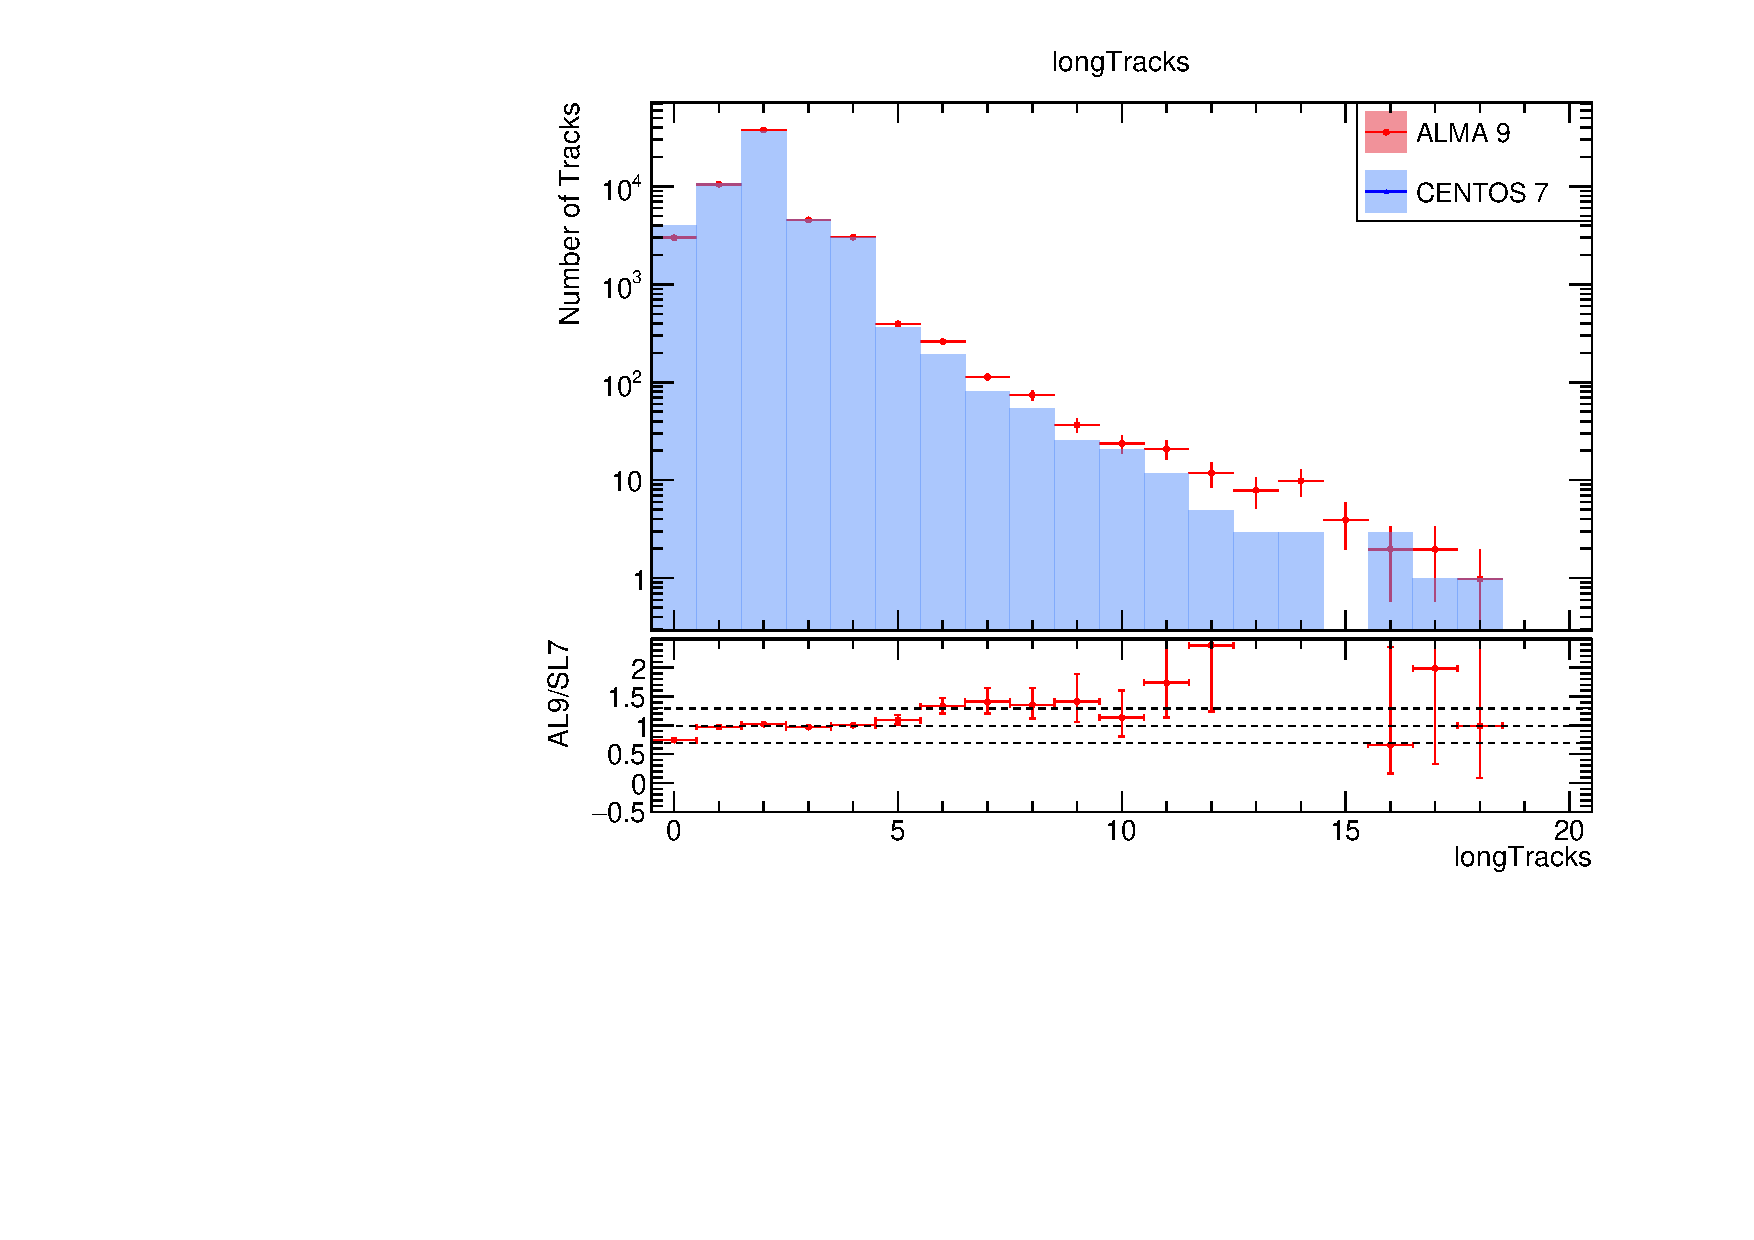
\includegraphics[width=\linewidth]{./output/longTracks.pdf}
        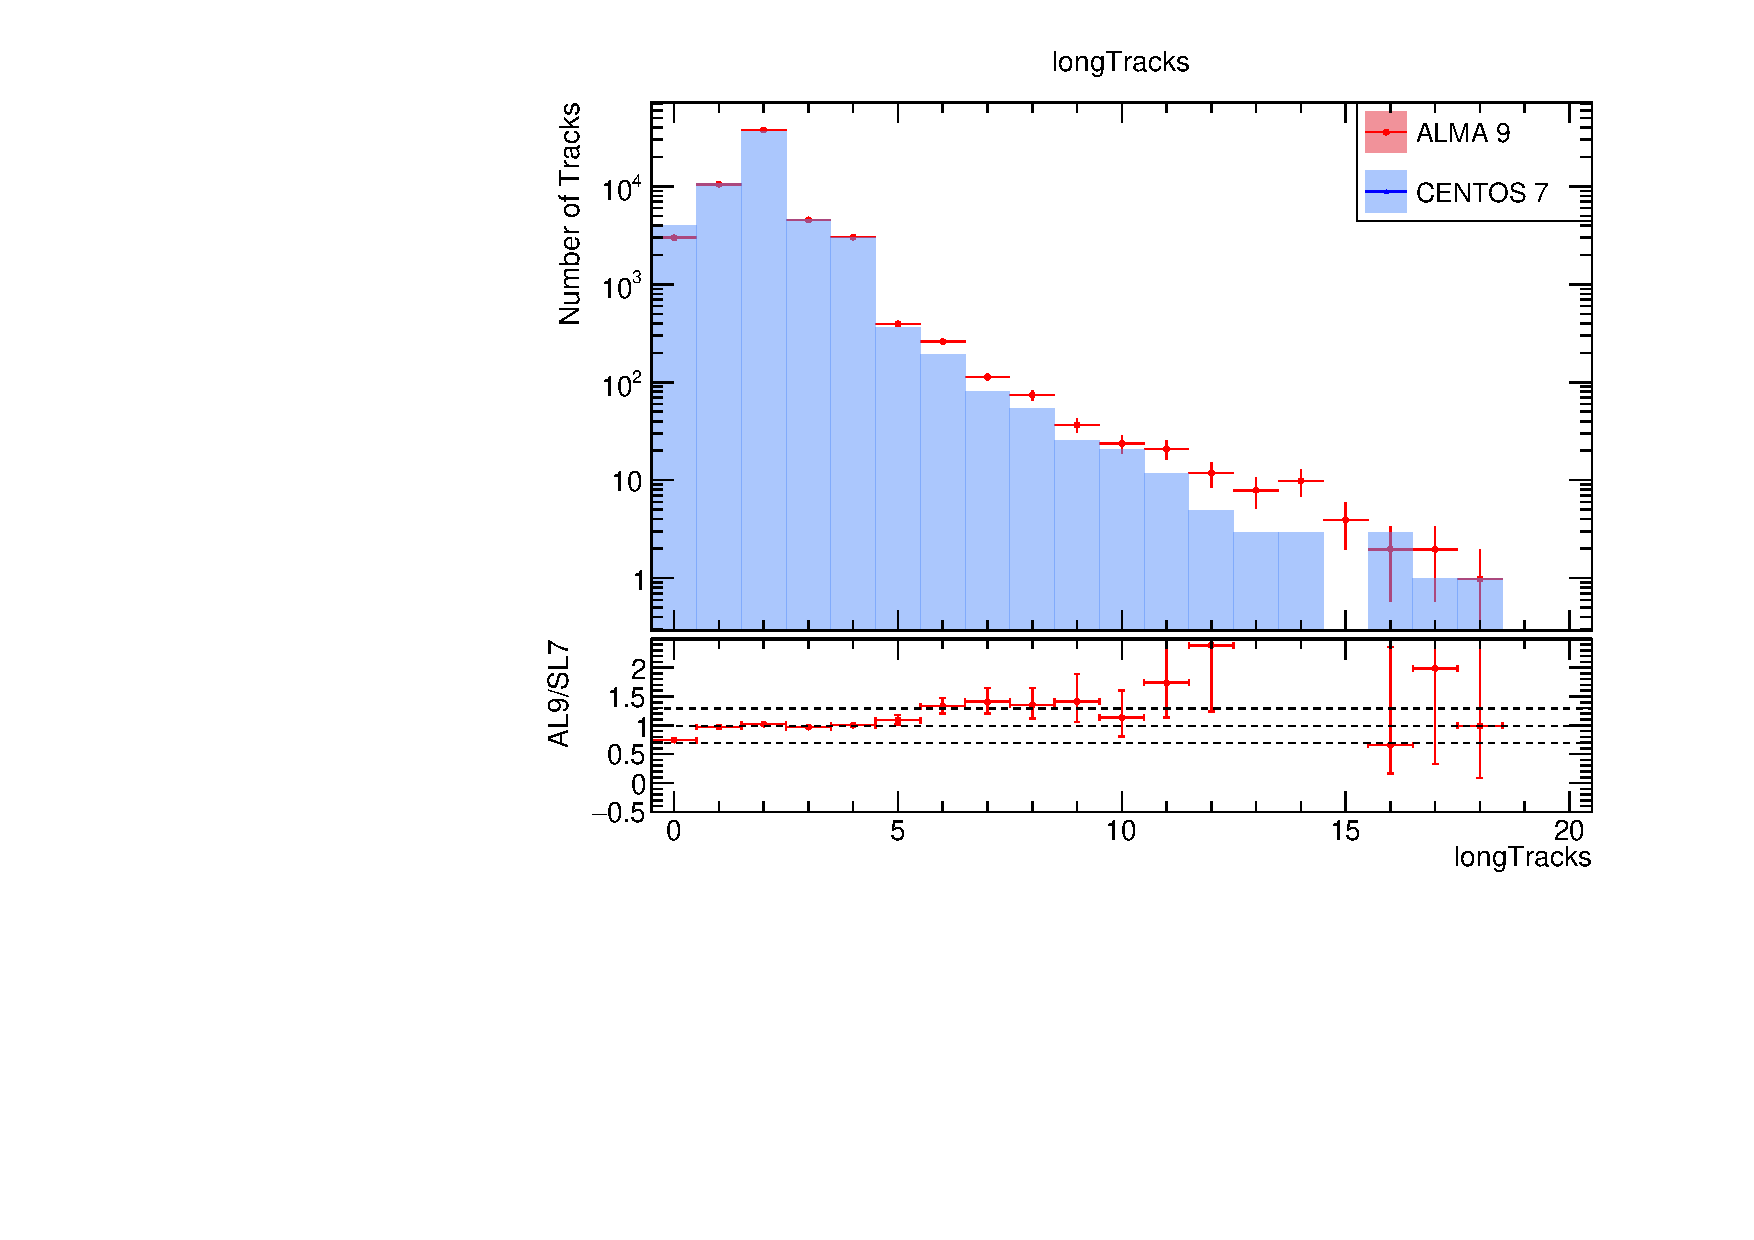
\includegraphics[width=0.8\linewidth]{output/longTracks.pdf}
    \end{figure}
    \vspace{-0.5cm}
    \begin{itemize}
        % \item Overall agreement is strong, especially in the early bins.
        \item \small ALMA9 has fewer 0-track events;
        \item \small Also reconstructs more events with more than 5 tracks.
        \item \small Total number of longTracks: CENTOS7: 115,206, AL9: 118,491
        \item \small A 2.8\% increase in longTracks in AL9.
        % \item longTracks \>5 shows more discrepancy, Concerning?
    \end{itemize}
\end{frame}


% \begin{frame}{Distribution of TrackPropagationError [SKIP]}
%     \begin{figure}
%         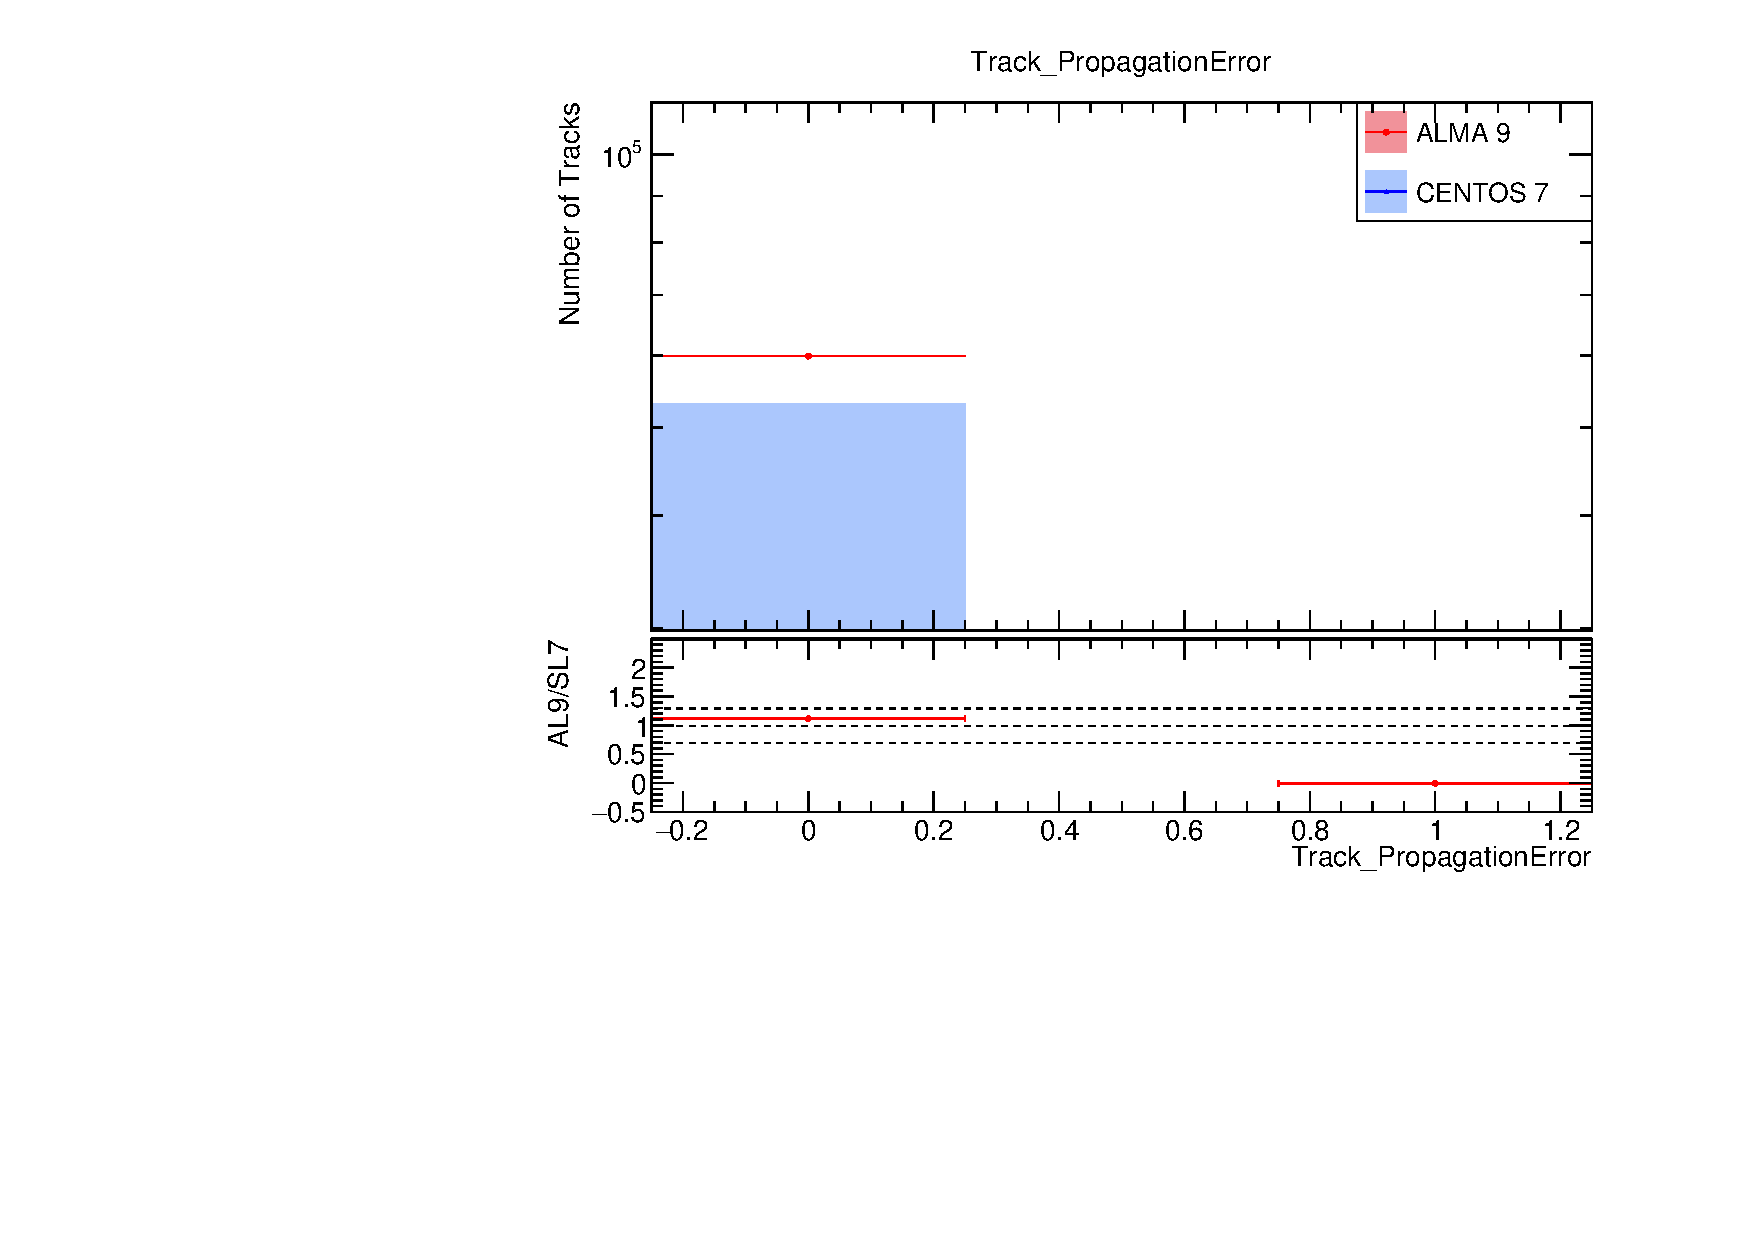
\includegraphics[width=0.9\linewidth]{output/Track_PropagationError.pdf}
%     \end{figure}
%     \vspace{-0.5cm}
%     \begin{itemize}
%         \item More TrackPropagationErrors in CENTOS7.
%     \end{itemize}
% \end{frame}

\begin{frame}{Distribution of TrackChi2}
    \begin{figure}
        \begin{subfigure}{0.49\linewidth}
            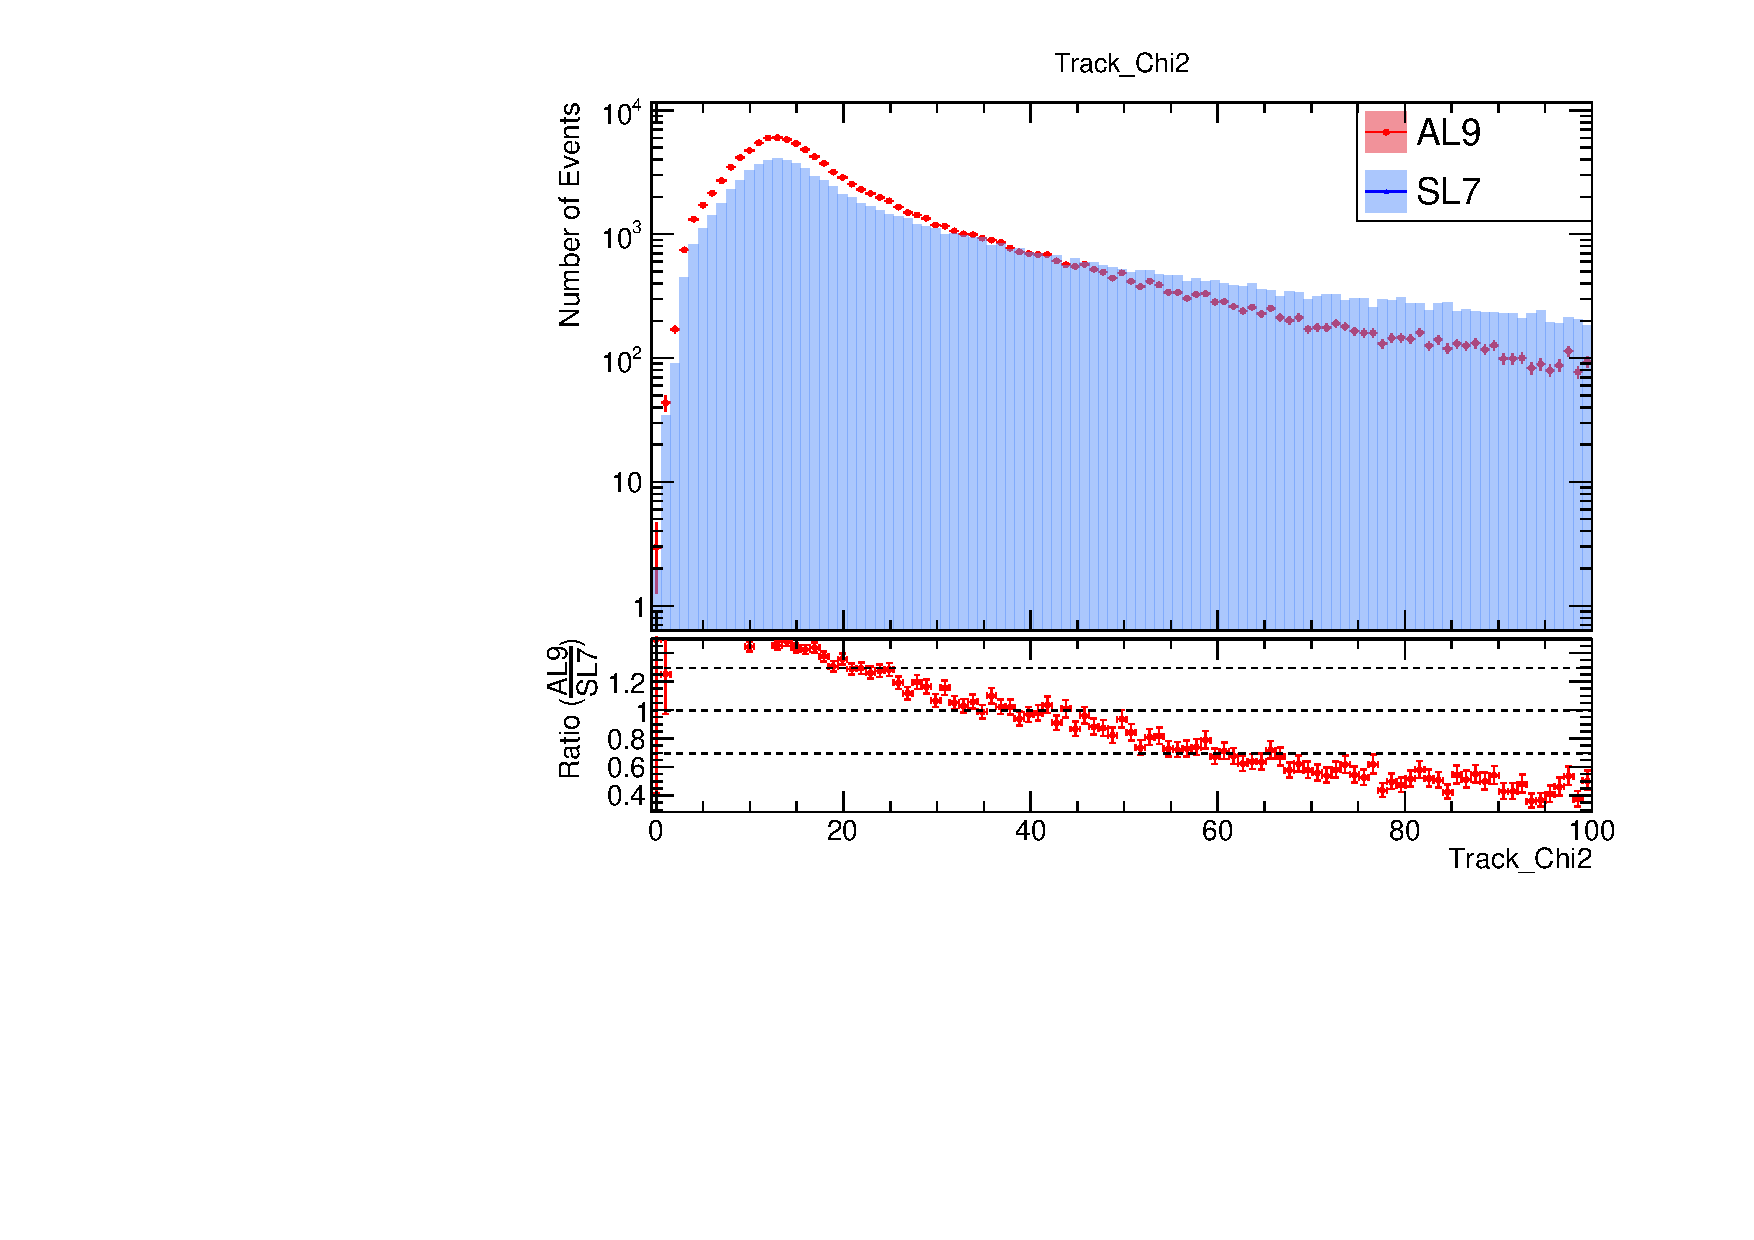
\includegraphics[width=\linewidth]{./output/Track_Chi2.pdf}
        \end{subfigure}
        \begin{subfigure}{0.49\linewidth}
            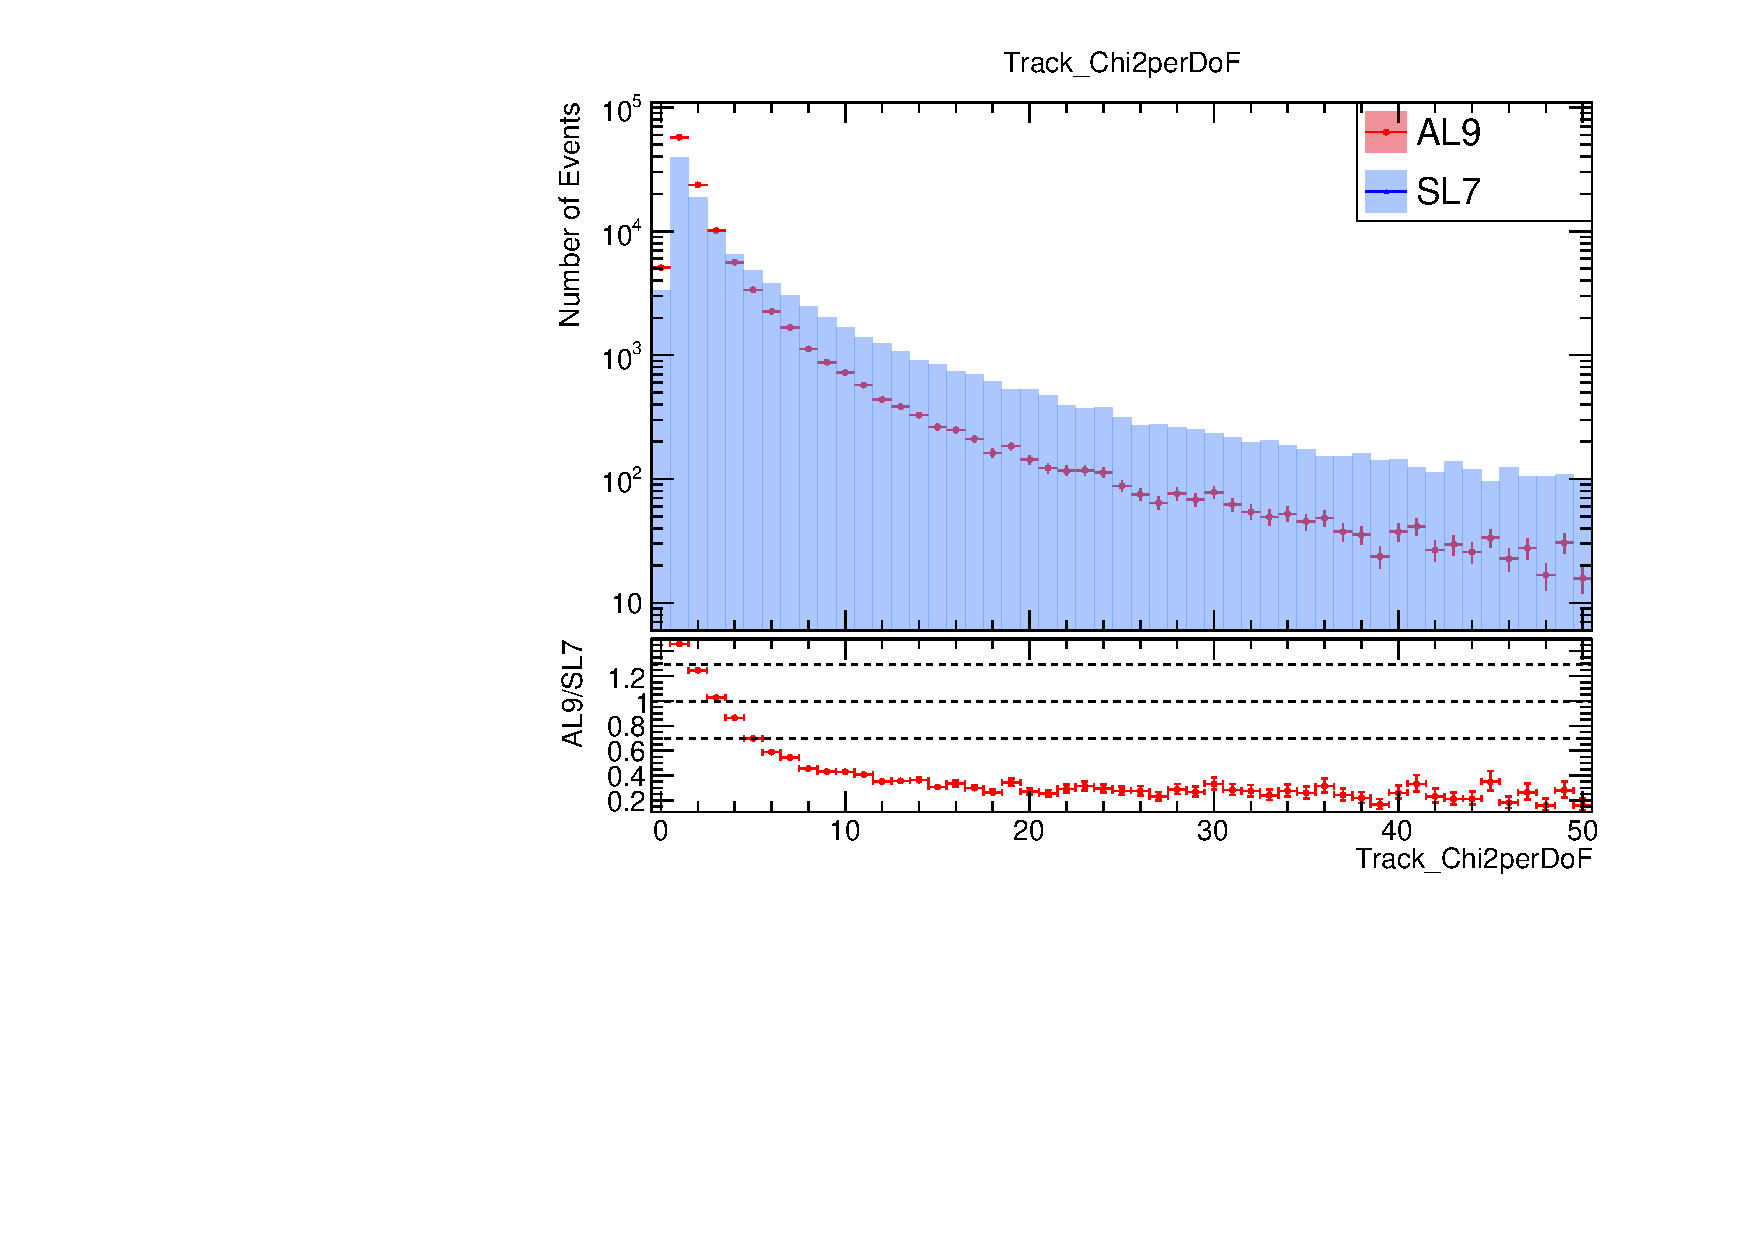
\includegraphics[width=\linewidth]{./output/Track_Chi2perDoF.pdf}
        \end{subfigure}
        \begin{itemize}
            \item Displays the greatest improvement in ALMA9.
            \item Overall Tracks have lower Chi2/DoF in ALMA9.
        \end{itemize}
    \end{figure}
\end{frame}

% \begin{frame}{Distribution of TrackChi2perDoF}
%     \begin{figure}
%         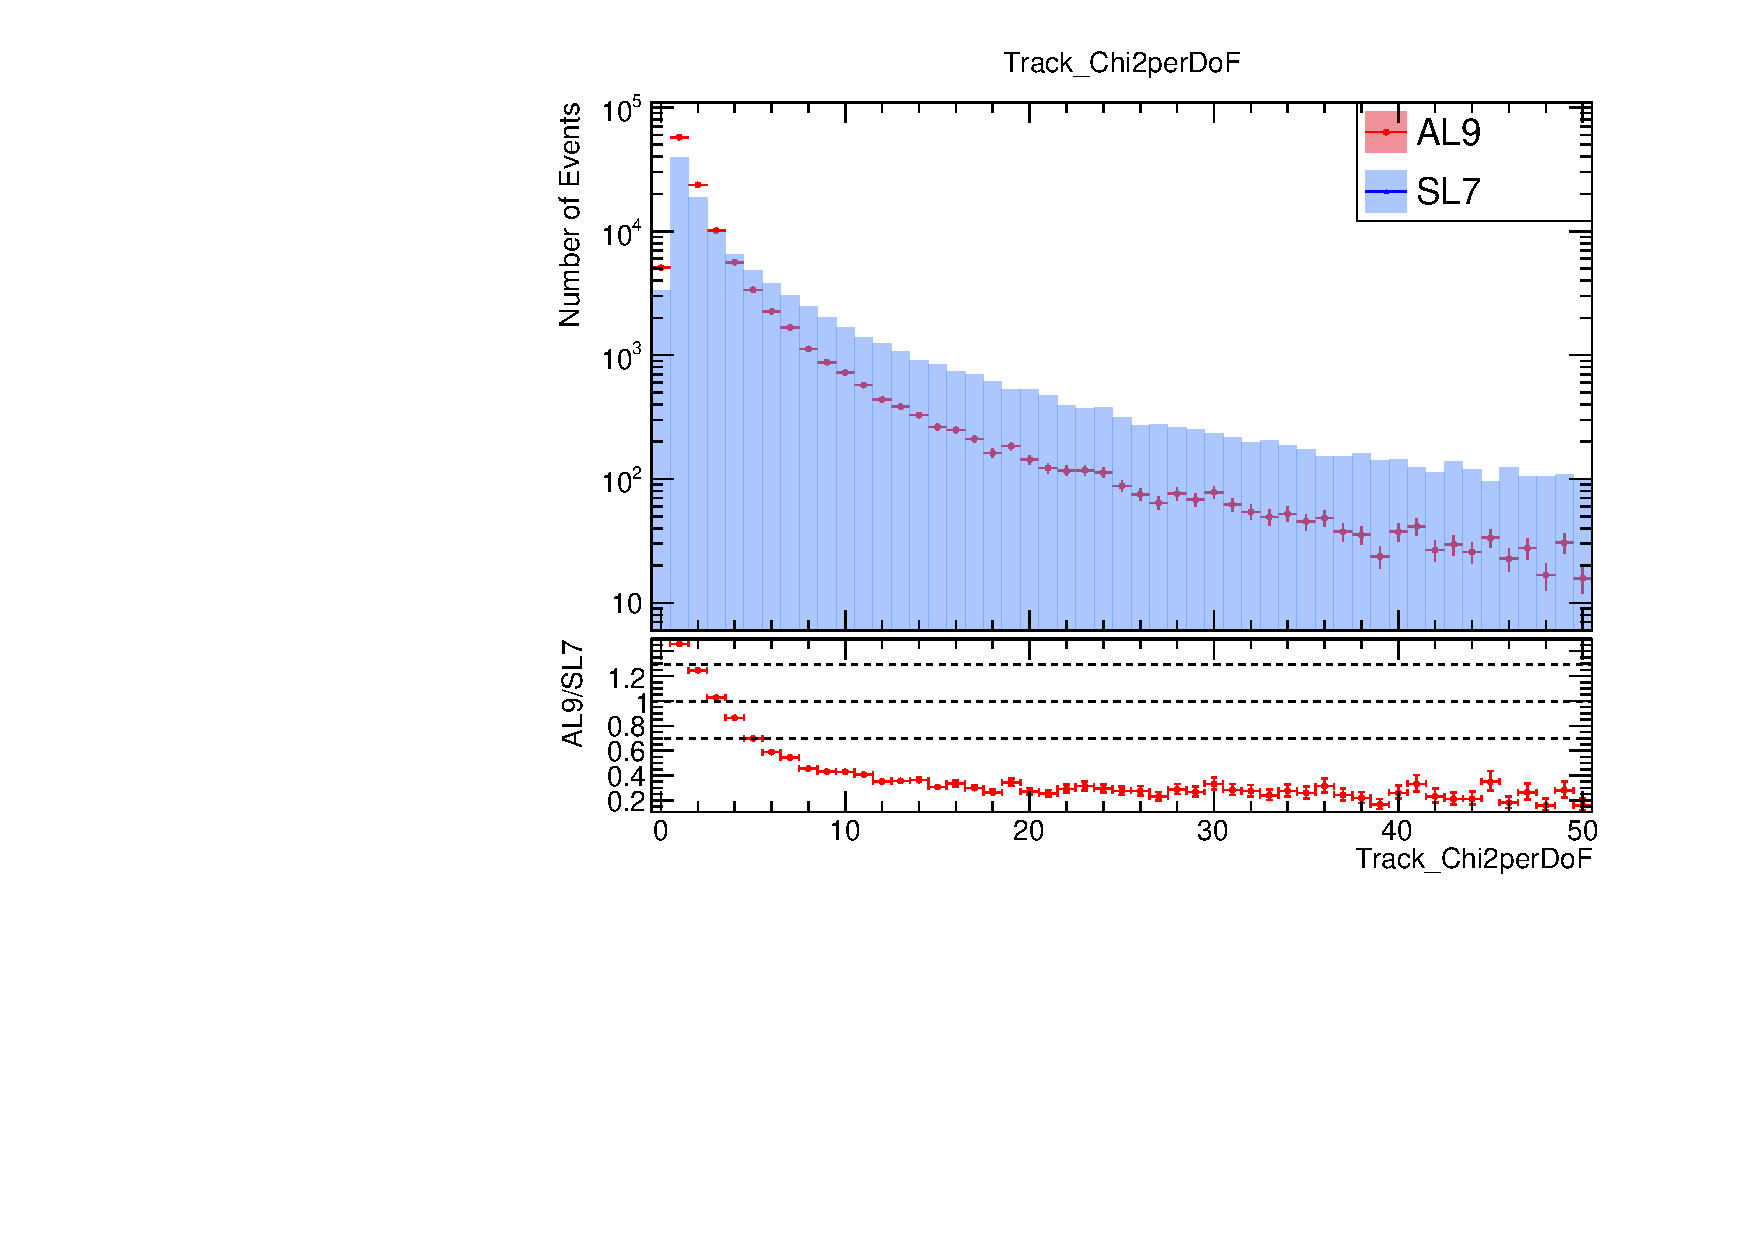
\includegraphics[width=0.9\linewidth]{./output/Track_Chi2perDoF.pdf}
%     \end{figure}
%     \vspace{-0.5cm}

% \end{frame}

\begin{frame}{Distribution of TrackNDoF}
    \vspace{-0.3cm}
    \begin{figure}
        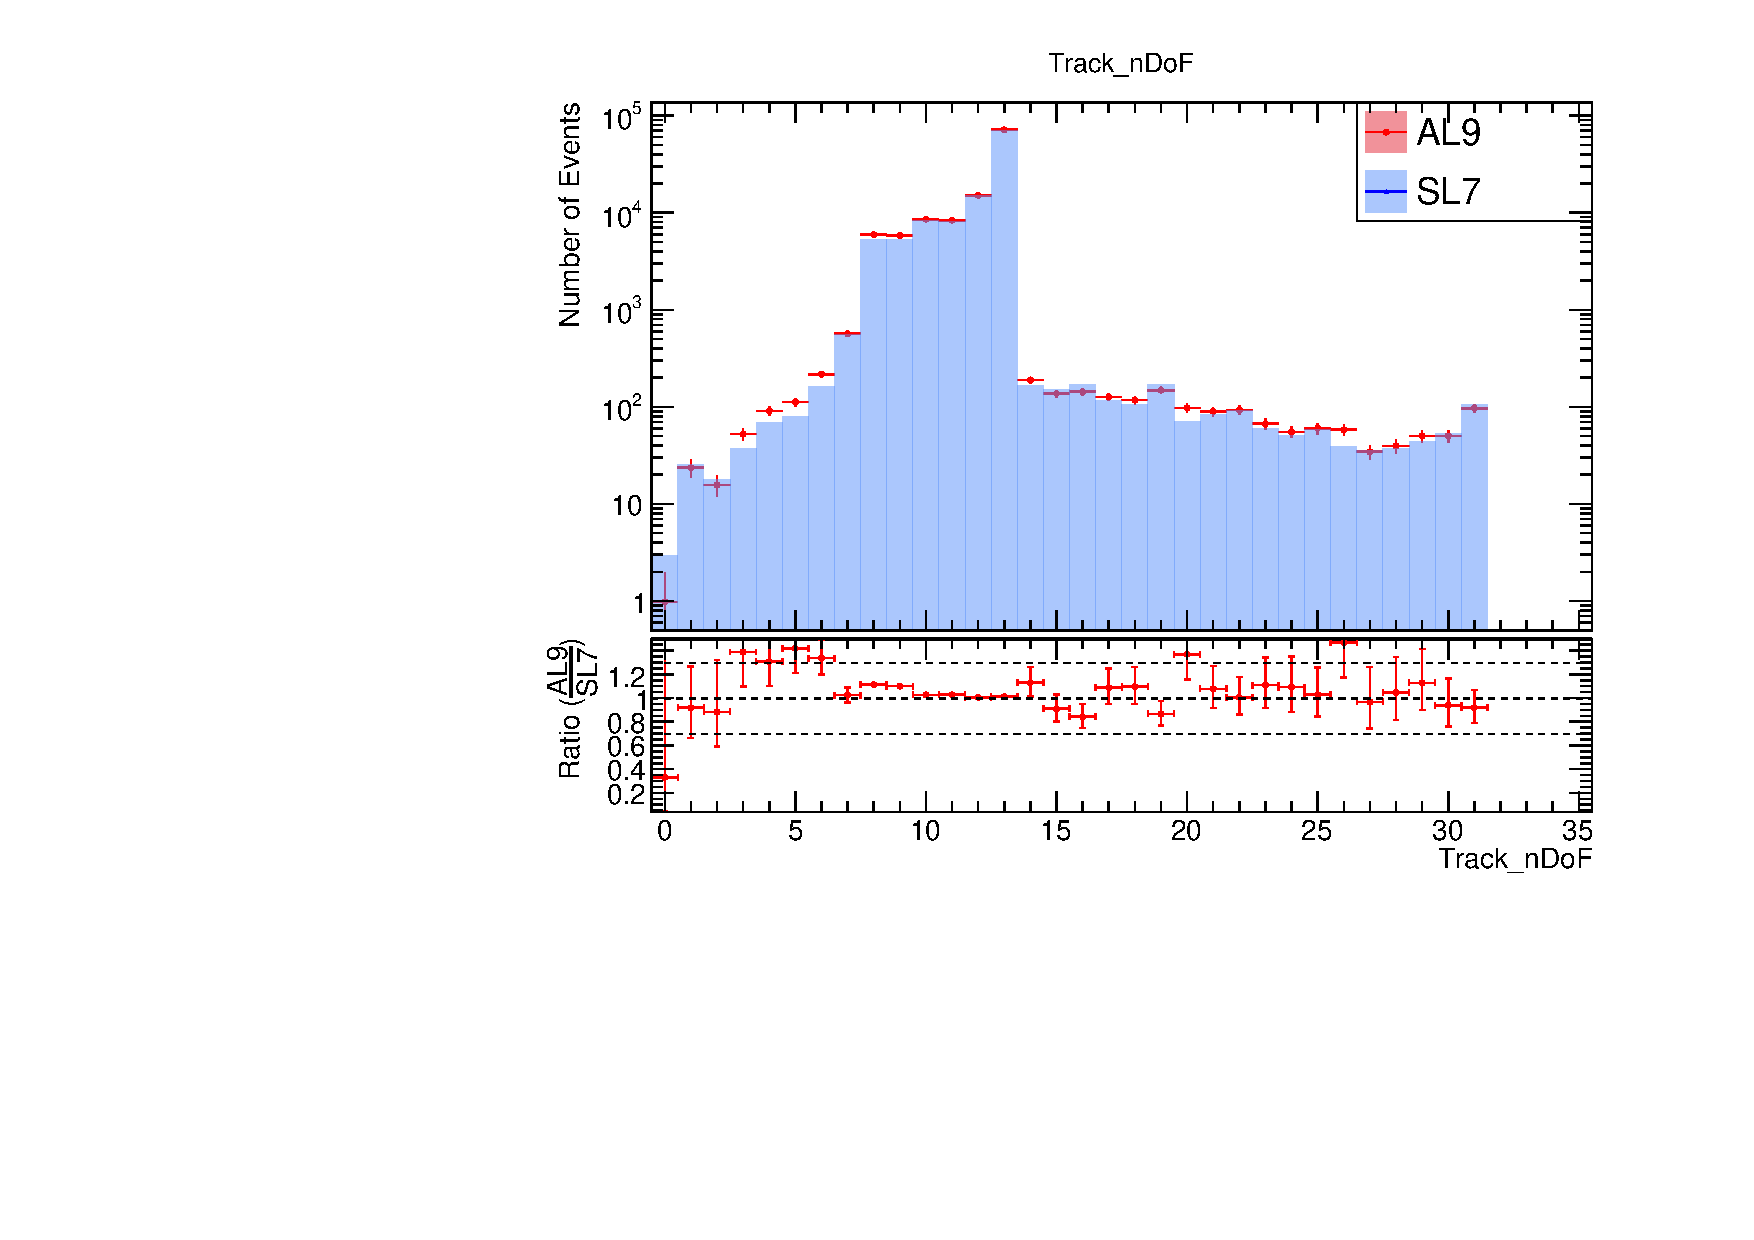
\includegraphics[width=\linewidth]{./output/Track_nDoF.pdf}
    \end{figure}
    \vspace{-0.65cm}
    \begin{itemize}
        \item Generally strong agreement, except for bins 3-5.
    \end{itemize}
\end{frame}

\begin{frame}{Distribution of Track Charge}
    \vspace{-0.3cm}
    \begin{figure}
        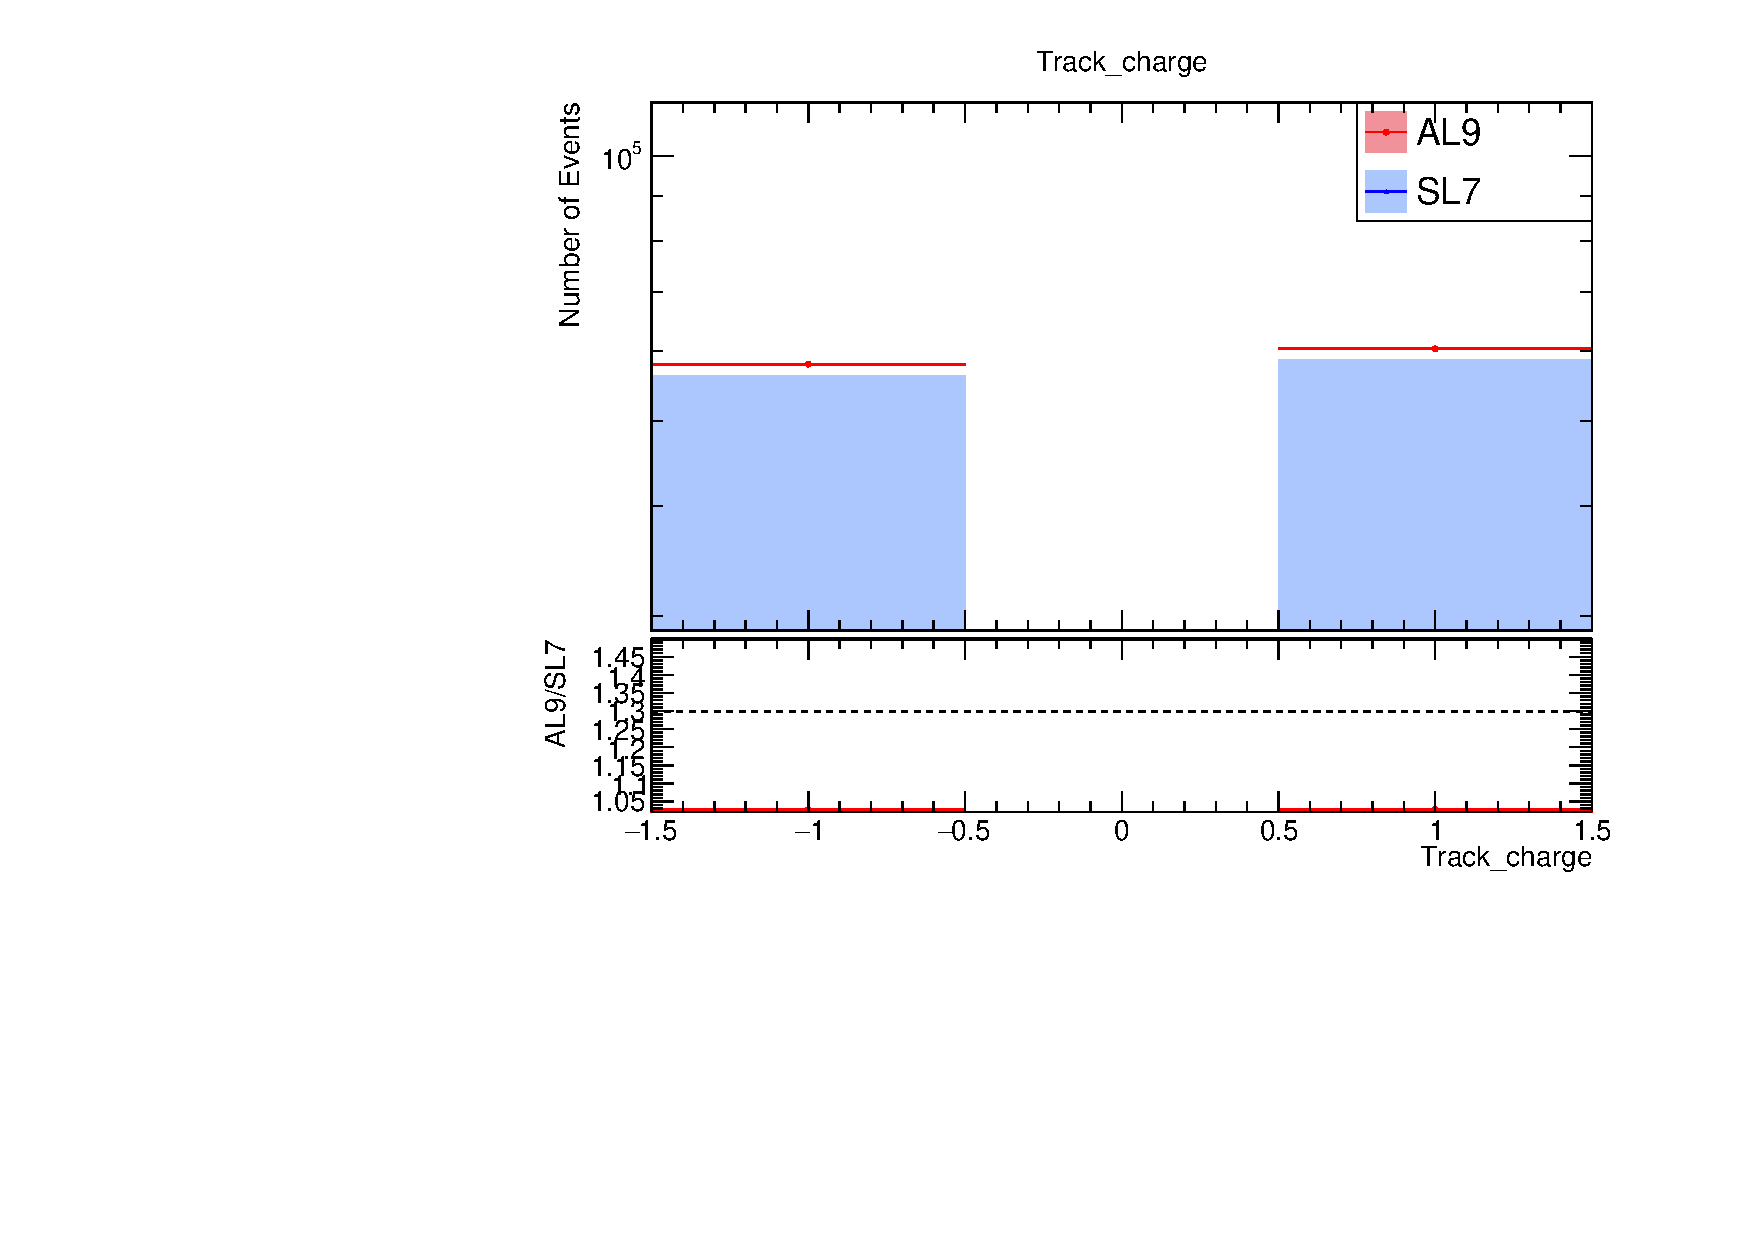
\includegraphics[width=0.9\linewidth]{./output/Track_charge.pdf}
    \end{figure}
    \vspace{-0.6cm}
        \begin{itemize}
            \item The ratio is 1.028 [same factor of increase seen in longTracks]
            \item Ratio of positive to negative tracks is 1.04. ChargeMisID?
        \end{itemize}
\end{frame}

\begin{frame}{Distribution of Track nLayers}
    \vspace{-0.3cm}
    \begin{figure}
        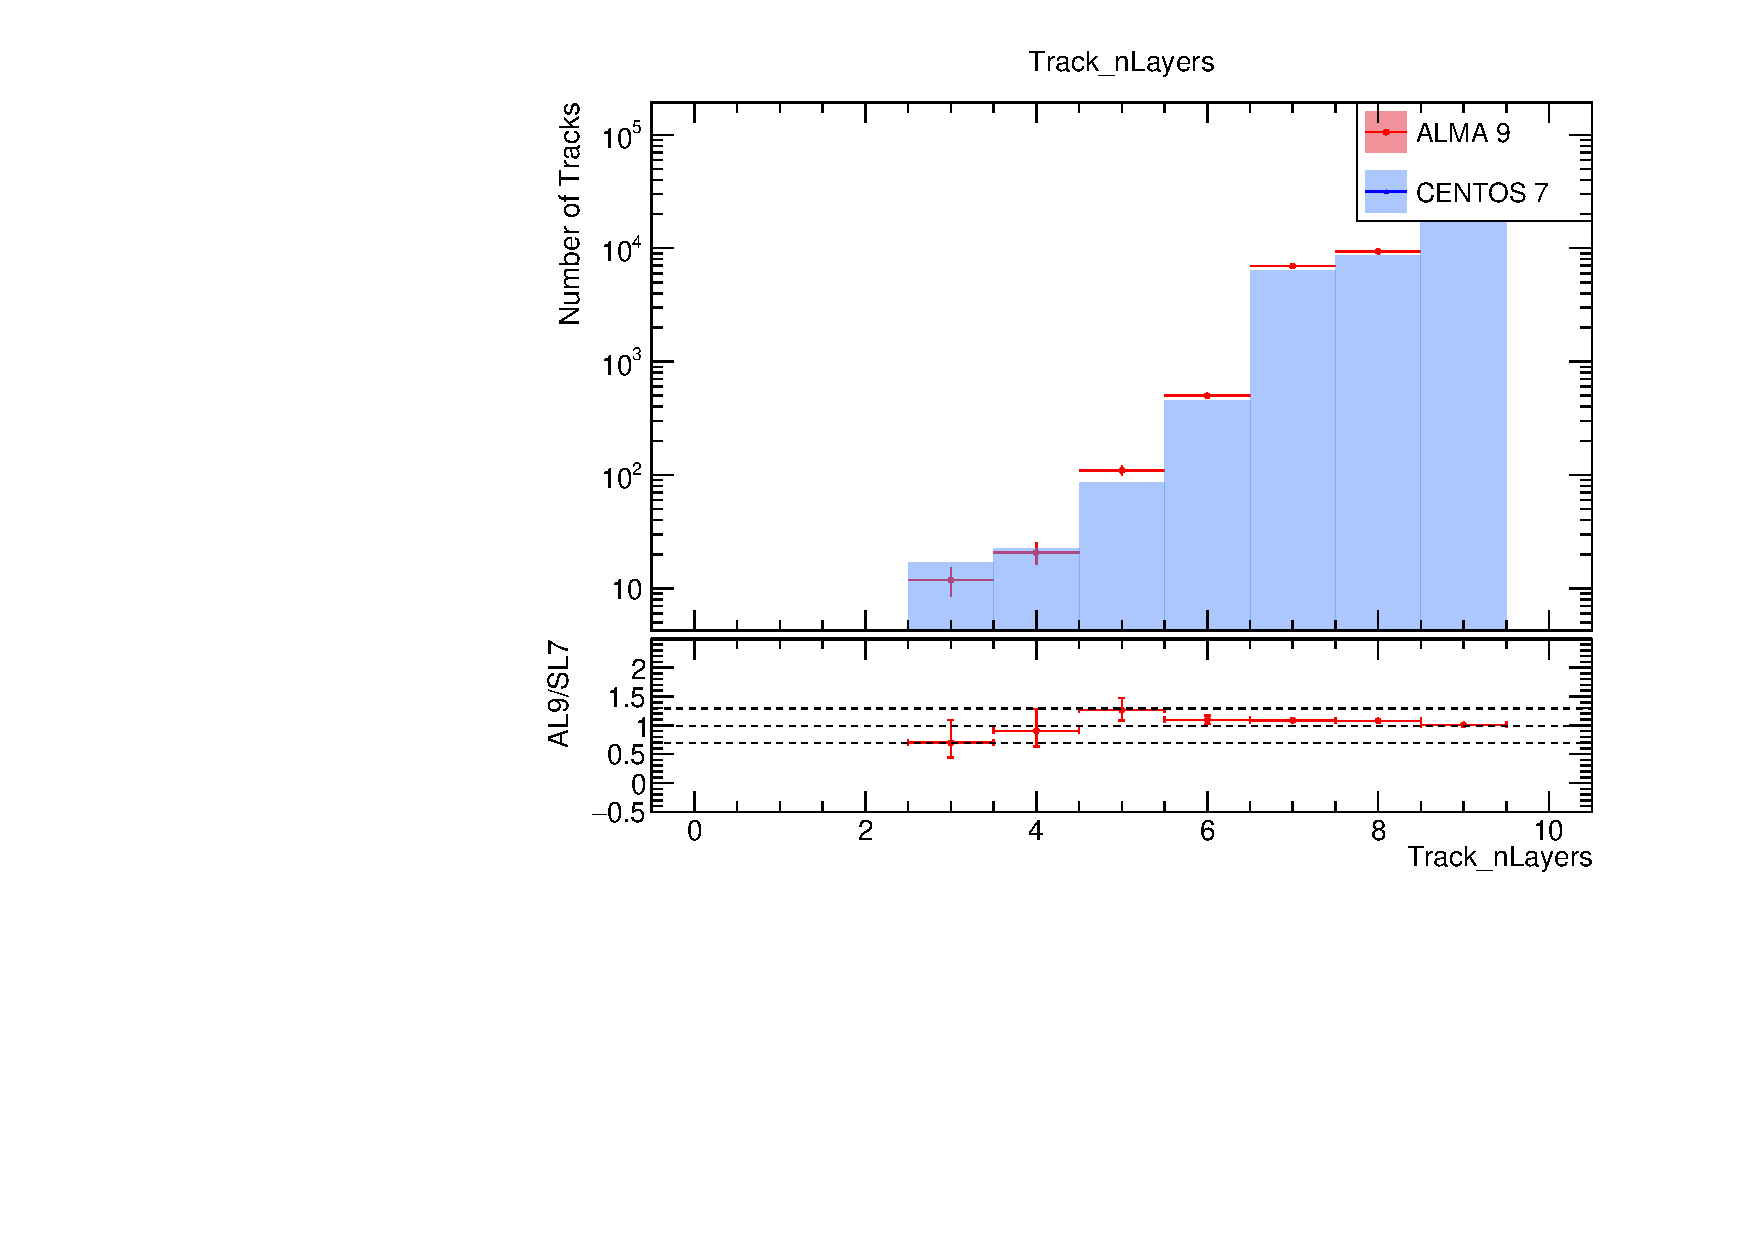
\includegraphics[width=0.95\linewidth]{./output/Track_nLayers.pdf}
    \end{figure}
    \vspace{-0.6cm}
    \begin{itemize}
        \item On average, more layers are hit (bins 5-8), but the high MC uncertainty makes it difficult to conclude definitively.
    \end{itemize}
\end{frame}

% \begin{frame}{Comments on Track Parameters}
%     \begin{itemize}
%         \item longTracks \> 5 is a mess, But not particularly useful
%         \item Track Propagation Error is a easily interpretable function
%         \item Track Chi2 changed a lot, much higher peak and lower tail in AL9, which is good.
%         \item TrackNDoF shows good agreement except betweeen 3-5
%         \item Track Charge in AL9 is slightly elevated, not sure why
%         \item Track nLayers is also decent agreement except at 5-8
%     \end{itemize}
% \end{frame}
\begin{frame}{Quantifying  Separation}
	Possible Track Separation Variables
	\begin{itemize}
		\item $\Delta R_0$ : Separation between the electron and positron at the first tracking station in the x-y plane
		\item $\Delta X_0$ : Same as above but only in x direction 
		\item $\Delta Y_0$ : Same as above but only in y direction
		\item $\theta_0$ : Angle between the line connection decay vertex to the two tracks at the first tracking station
		% \item $\Phi_{p0}$ [To be Removed]
		\item $\Delta R_P = \sqrt{\Delta \eta ^2 + \Delta \phi^2}$  : Momentum space separation between electron and positron
	\end{itemize}
\end{frame}



\begin{frame}{Position Based Separation variables}
	\begin{figure}
		
	% Showing Various Separation
	\begin{tikzpicture}[scale=1]
	% Draw grid
	\draw[step=1cm,gray!30,very thin] (-2,-1) grid (5,5);
	
	\coordinate (a) at (1,1);
	\coordinate (b) at (3,4);
	
	% Draw axes
	\draw[->,thick] (-1,0) -- (0,0) node[right] {$x$};
	\draw[->,thick] (-1,0) -- (-1,1) node[above] {$y$};
	% Mark Origin
	% \node[below right] at (0,0) {$(0,0)$};
	
	% Draw and label the points
	\filldraw (a) circle (2pt) node[below left] {electron (d1)};
	\filldraw (b) circle (2pt) node[above right] {positron (d0)};
	
	% Draw delta x, delta y
	\draw[->,thick,blue] (b) -- (a -| b) node[midway,right] {$\Delta Y0$};
	\draw[<-,thick,blue] (a) -- (a -| b) node[midway,below] {$\Delta X0$};
	
	% Draw delta r
	\draw[<->,thick,red] (b) -- (a) node[midway,above left] {$\Delta R0$};
	\end{tikzpicture}
	\caption{Tracking Station 1}
	\end{figure}

	ADD CODE SNIPPET
\end{frame}

\begin{frame}{Track Separation in terms of Angle}
	\begin{figure}
		\begin{tikzpicture}[scale=1]
			% Define Mother and daughter particles
			\coordinate(M) at (-1, 0);
			\coordinate(d1) at (3, 1);
			\coordinate(d2) at (3, -1);
		
			% Draw grid
			\draw[step=1cm,gray!30,very thin] (-2.5, -2) grid (4.5, 2);
			\draw[-,thick] (3,-2) -- (3,2) node[pos=0.95, left] {Tracking Station 1};
			\draw[->, thick](3, 0) -- (3.5, 0) node[right] {$z$};
			
			% Draw mother and daughter particles
			\filldraw (M) circle (2pt) node[above left] {Dark-Photon (M)};
			\filldraw (d1) circle (2pt) node[above right] {positron (d0)};
			\filldraw (d2) circle (2pt) node[above right] {electron (d1)};
		
			\draw[dashed] (M) -- (d1);
			\draw[dashed] (M) -- (d2);
		
		% Draw arc and label the angle
		\draw[<->, thick, red] (M)+({atan(1/4)}:1) arc ({atan(1/4)}:{atan(-1/4)}:1) node[midway, right] {$\theta$};
		
		\end{tikzpicture}
		\caption{Angle between Tracks}	
		ADD CODE SNIPPET
	
	\end{figure}
	
\end{frame}

% \begin{frame}{Track Separation in terms of Momenta [Not Good]}
% 	\begin{figure}
% 	\begin{tikzpicture}[scale=1]
% 		% Define Daughter particles
% 		\coordinate(d1) at (3, 1);
% 		\coordinate(d2) at (3, -1);
	
% 		% Draw grid
% 		\draw[step=1cm,gray!30,very thin] (1, -3) grid (7, 3);
% 		\draw[-,thick] (3,-2) -- (3,2) node[pos=0.95, left] {Tracking Station 1};
% 		\draw[->, thick](3, 0) -- (3.5, 0) node[right] {$z$};
	
		
% 		% Daughter particles
% 		\filldraw (d1) circle (2pt) node[below left] {+ve charged (d0)};
% 		\filldraw (d2) circle (2pt) node[above left] {-ve charged (d1)};
	
% 		% Make Momentum Vectors
% 		\draw[->, thick, red]  (d1) -- ($(d1)+(1, 0.5)$) node[right] {$\vec{p_0}$};
% 		\draw[->, thick, blue] (d2) -- ($(d2)+(1, -0.5)$) node[right] {$\vec{p_1}$};
	
% 		% Show Translation
% 		\draw[dashed, red] (d1) -- (4, 0);
% 		\draw[dashed, red] ($(d1)+(1, 0.5)$) -- ($(4, 0) + (1, 0.5)$);
% 		\draw[dashed, blue] (d2) -- (4, 0);
% 		\draw[dashed, blue] ($(d2)+(1, -0.5)$) -- ($(4, 0) + (1,- 0.5)$);
	
% 		% Show angle between vectors
% 		\draw[->, thick, red] (4, 0) -- (5, 0.5) node[right] {$\vec{p_1}$};
% 		\draw[->, thick, blue] (4, 0) -- (5, -0.5) node[right] {$\vec{p_0}$};
% 		\draw[<->, thick] (4,0) + ({atan(-0.5/1)}:0.6) arc ({atan(-0.5/1)}:{atan(0.5/1)}:0.6) node[midway, right] {$\Phi_p$};
	
% 	\end{tikzpicture}
% 	\caption{Angle between Momenta}
% 	\end{figure}
% \end{frame}

\begin{frame}{Track Separation in $\eta$ - $\phi$ Space}
	\begin{figure}
	\begin{tikzpicture}[scale=1]
		% Define Daughter particles
		\coordinate(d1) at (0, 0);
		\coordinate(d2) at (0, 0);
	
		% Draw grid
		\draw[step=1cm,gray!30,very thin] (-1, -2) grid (3, 2);
		\draw[->, thick](-1, -2) -- (2.5, -2) node[right] {$\eta$};
		\draw[->, thick](-1, -2) -- (-1, 2) node[above] {$\phi$};
	
		
		% Daughter particles
		\filldraw (d1) circle (2pt); %node[below left] {+ve charged (d0)};
		\filldraw (d2) circle (2pt); %node[above left] {-ve charged (d1)};
	
		% Make Momentum Vectors
		\draw[->, thick, red]  (d1) -- ($(d1)+(1.5, 1)$) node[right] {$\vec{p_0}$ (d0)};
		\draw[->, thick, blue] (d2) -- ($(d2)+(1.5, -1)$) node[right] {$\vec{p_1}$ (d1)};
		\draw[<->, thick] (0,0) + ({atan(-1/1.5)}:0.6) arc ({atan(-1/1.5)}:{atan(1/1.5)}:0.6) node[midway, right] {$\Delta R_P$};
		
	
	\end{tikzpicture}
	\caption{Angle between Momenta}
	\end{figure}

\end{frame}

\begin{frame}{Code Sinppets}
	TODO: Fix listing here
% 	\begin{verbatim}
% 		XYZVector d0(truthd0_x[i], truthd0_y[i], truthd0_z[i]);
% 		Double_t deltaR = sqrt(pow(antimuon_at_station.X() - muon_at_station.X(), 2) + pow(antimuon_at_station.Y() - muon_at_station.Y(), 2));

% 		PxPyPzEVector d0(truthd0_px[i], truthd0_py[i], truthd0_px[i], truthd0_P[i]);
% 		Double_t deltaR = ROOT::Math::VectorUtil::DeltaR(antimuon_at_station, muon_at_station);
% 		XYZVector antimuon_at_station = d0_positions[1];
% 		XYZVector muon_at_station = d1_positions[1];

% 		Double_t deltaY = antimuon_at_station.Y() - muon_at_station.Y();
% 		Double_t deltaX = antimuon_at_station.X() - muon_at_station.X();
% 		Double_t deltaZ = (antimuon_at_station.Z() + muon_at_station.Z())*0.5 - (d0_positions[0].Z() + d1_positions[0].Z())*0.5;
% 		Double_t deltaR = sqrt(pow(deltaX, 2) + pow(deltaY, 2));
% 		Double_t theta = atan2(deltaR, deltaZ);
% 		\end{verbatim}
\end{frame}

\begin{frame}{Distribution of DeltaR0}
	\begin{figure}
		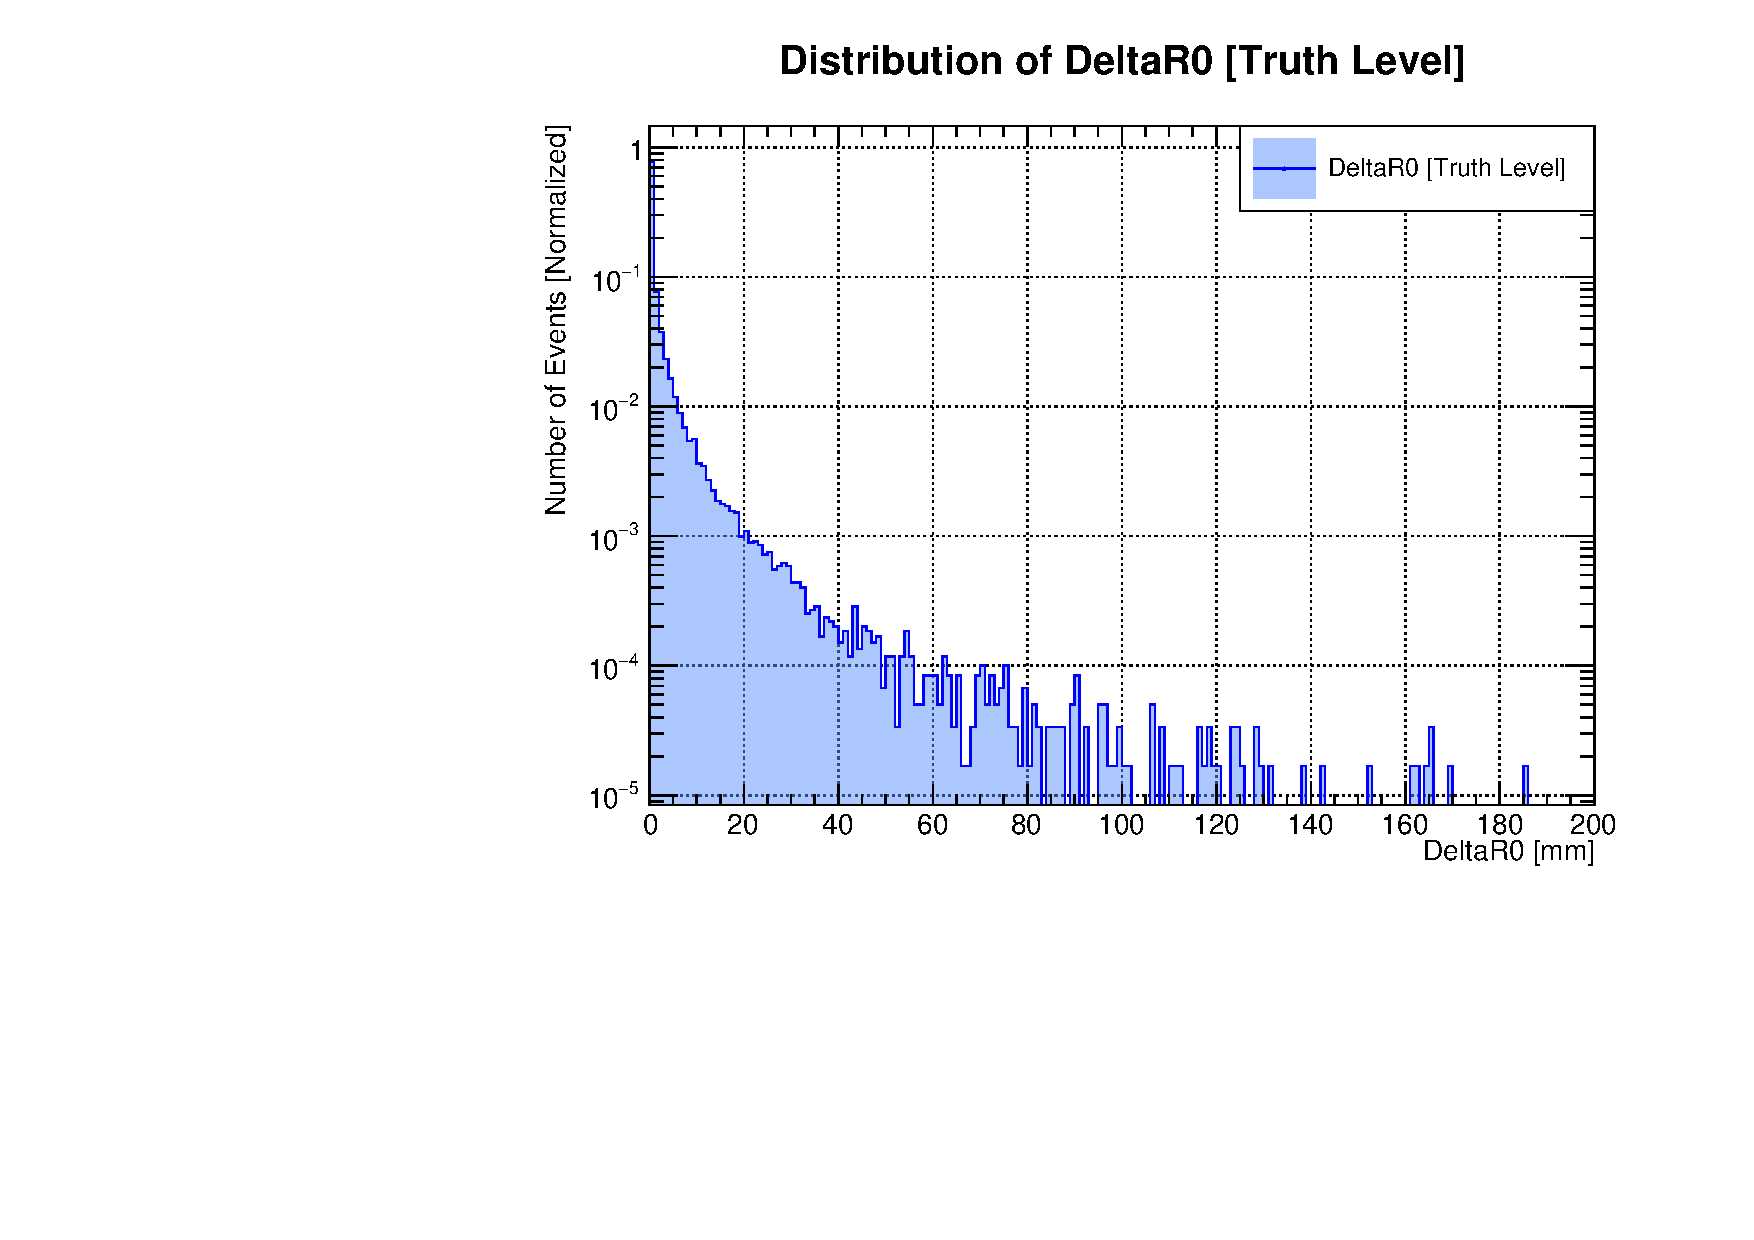
\includegraphics[width=\linewidth]{./output/DeltaR0.pdf}
	\end{figure}
\end{frame}

\begin{frame}{Distribution of DeltaX0}
	\begin{figure}
		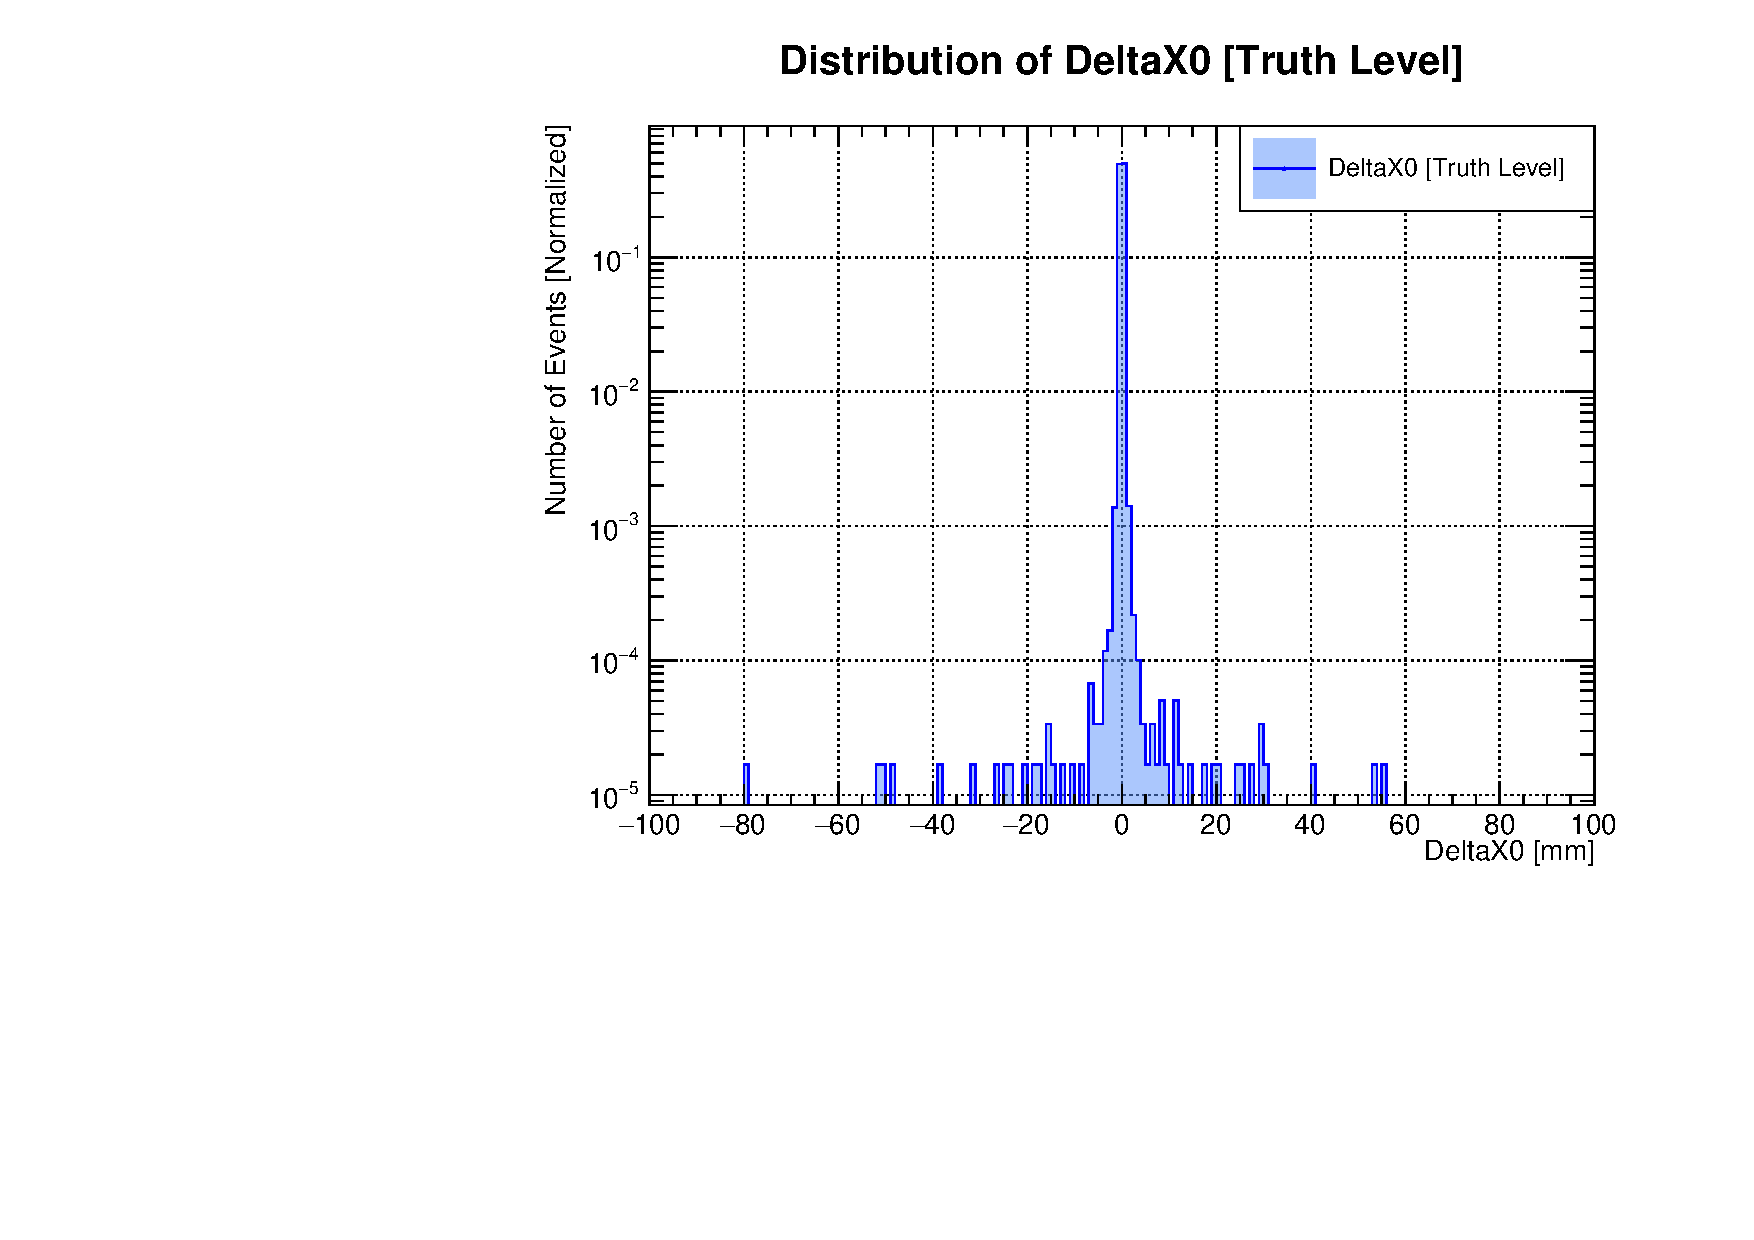
\includegraphics[width=\linewidth]{./output/DeltaX0.pdf}
	\end{figure}
\end{frame}

\begin{frame}{Distribution of DeltaY0}
	\begin{figure}
		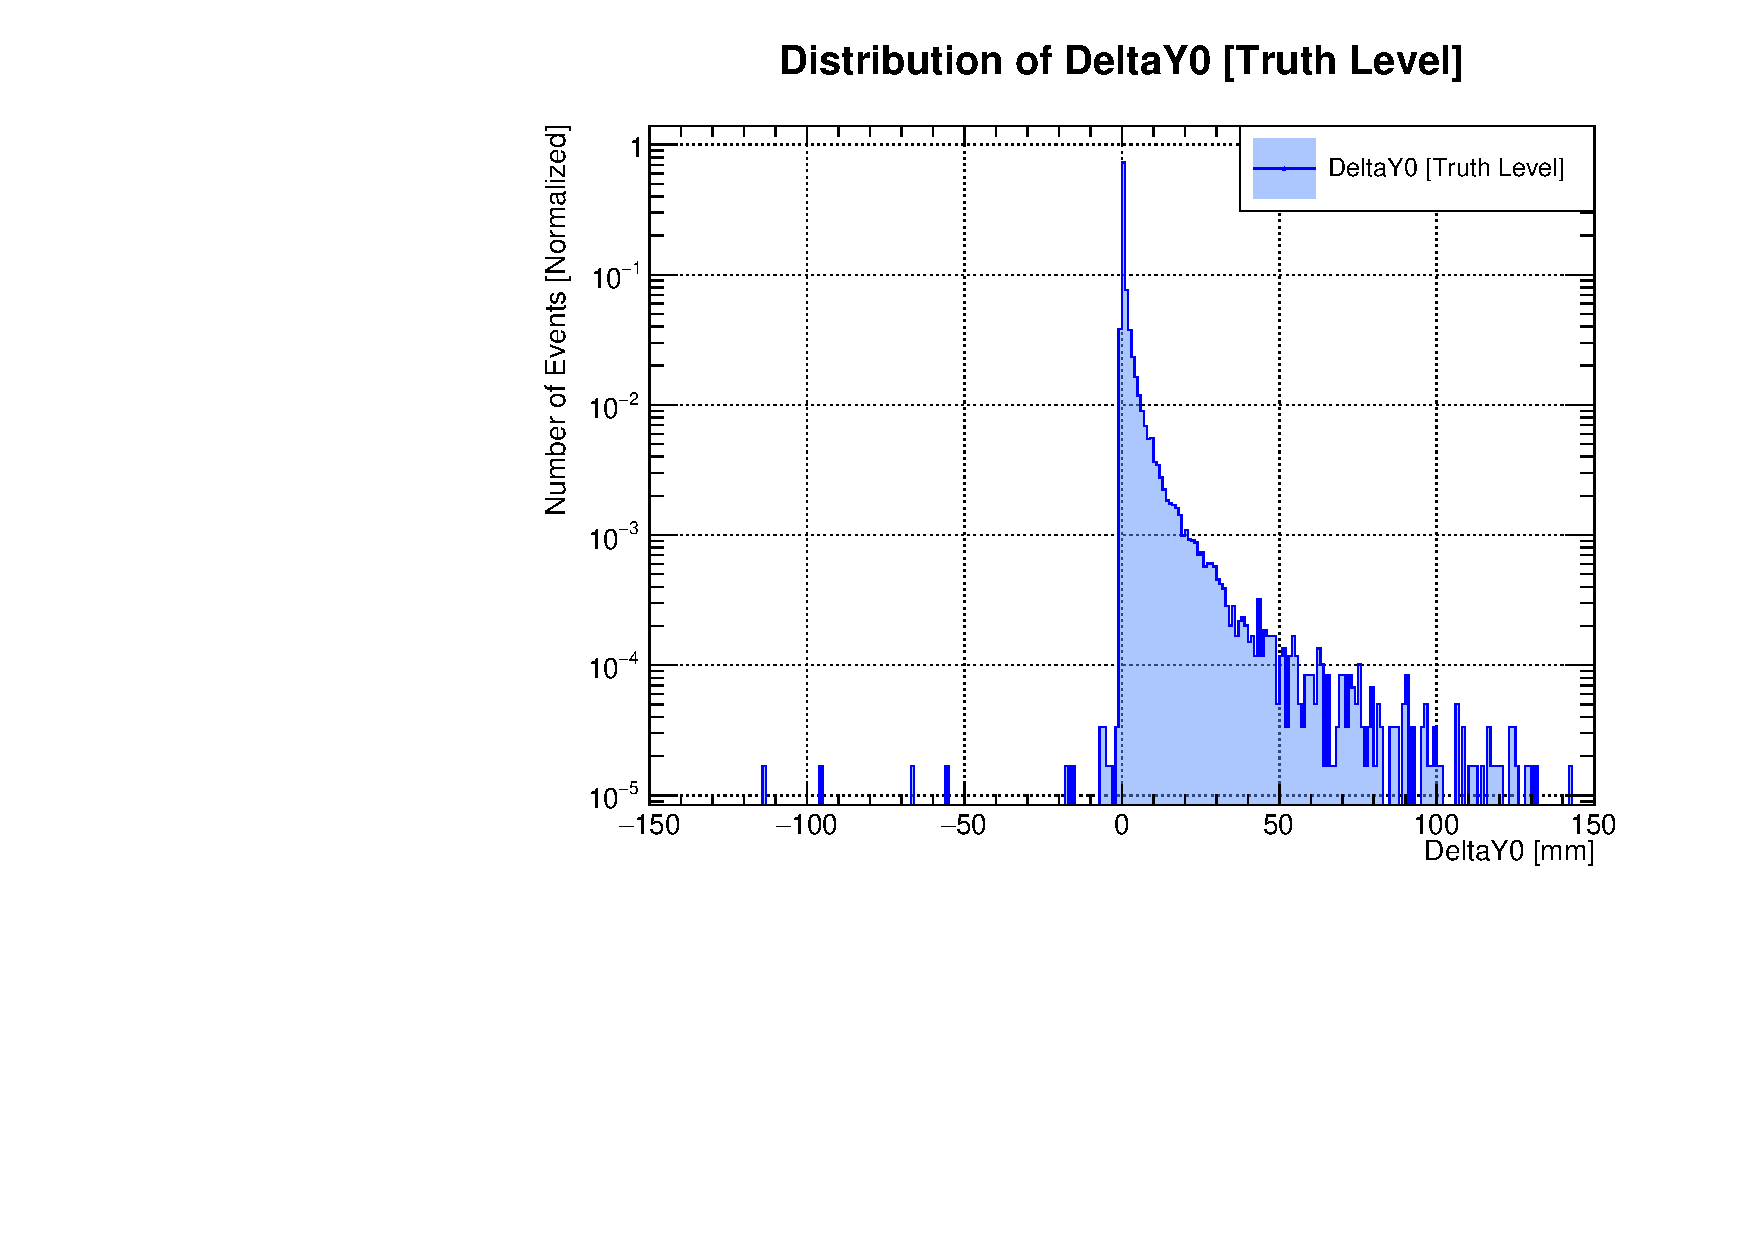
\includegraphics[width=\linewidth]{./output/DeltaY0.pdf}
	\end{figure}
\end{frame}

\begin{frame}{Comments on Position Based Separation}
		\begin{itemize}
			\item Particle predominantly separated in the y-direction
			\begin{itemize}
				\item Comes from the magentic field's deflection
				\item Positron deflected upwards, electron downwards leading asymmetry in DeltaY0 plot
				\item DeltaX0 looks symmetric
				\item DeltaY0 can be approximated to DeltaR0
			\end{itemize}
			\item In general Nevents fall off as sepration increases [characteristic of DP Decay?]
			\item Similar features seen in overlay plot but different in scale
			\item We can just look at the distributions using DeltaR0 as our primary variable for position based separation.
		\end{itemize}
		% \begin{figure}
		% 	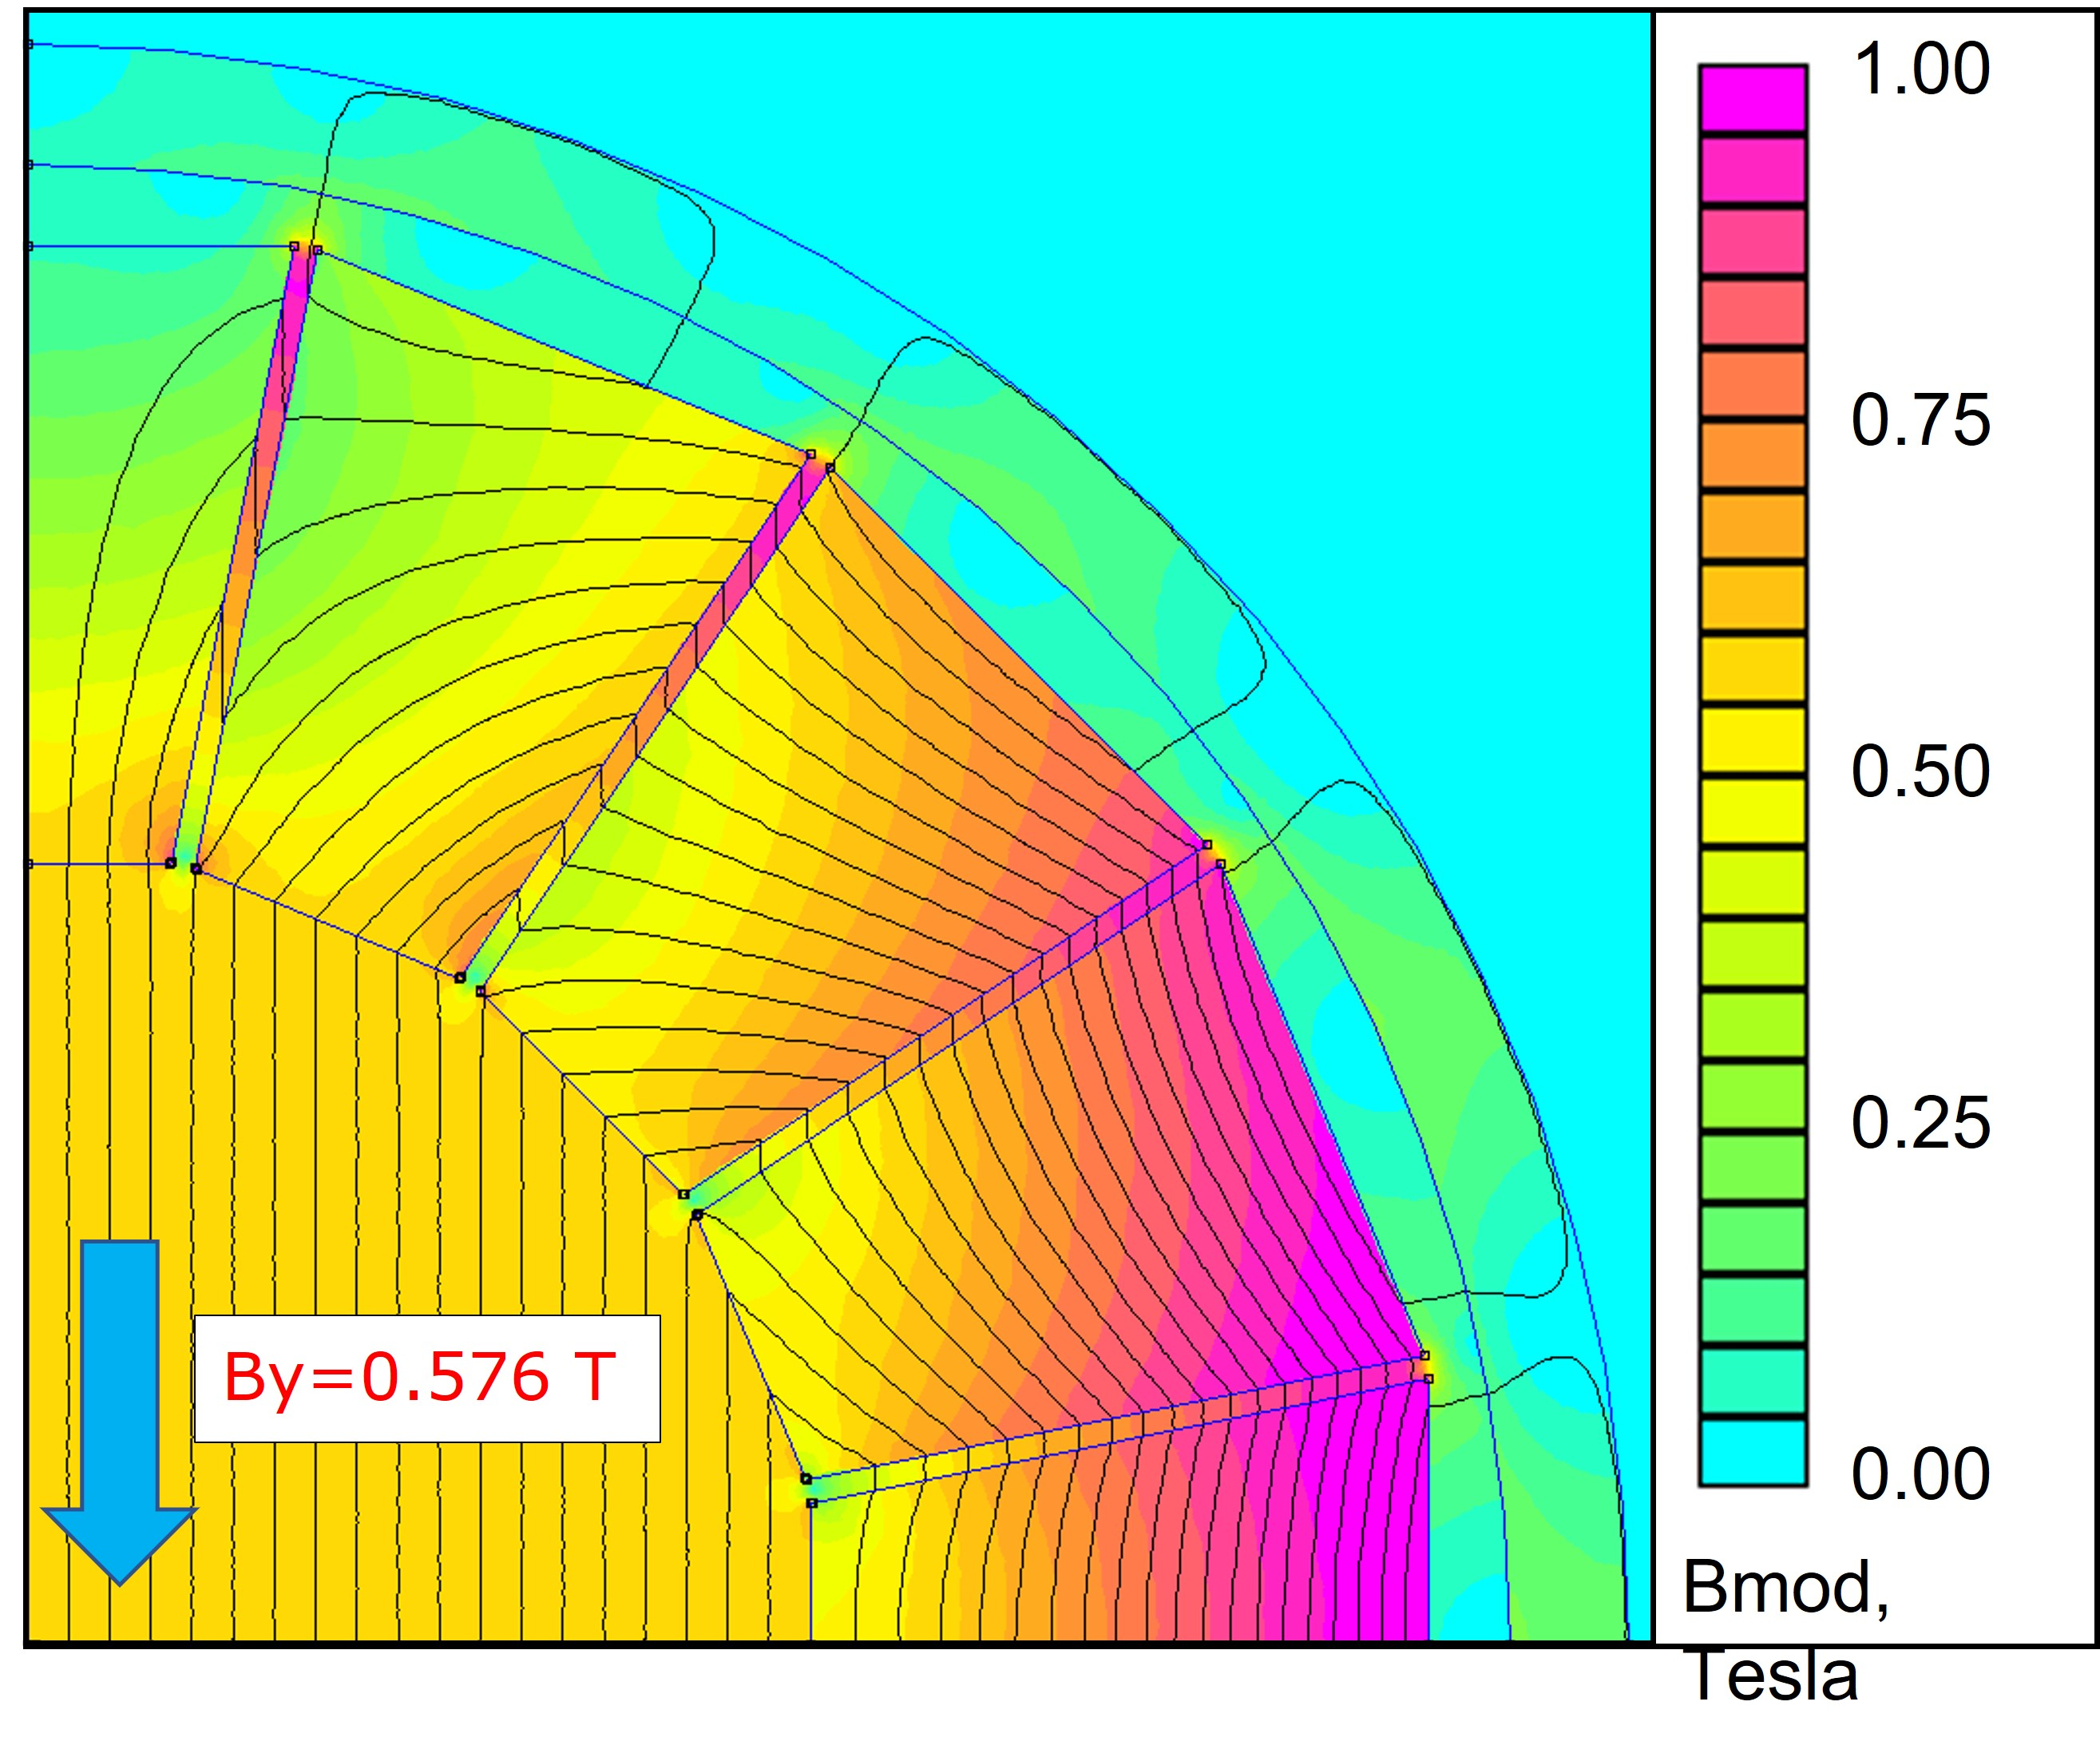
\includegraphics[width=0.5 \linewidth]{./assets/FASERMagField.png}
		% \end{figure}
\end{frame}

\begin{frame}{Overlay Plot}
	\begin{figure}
		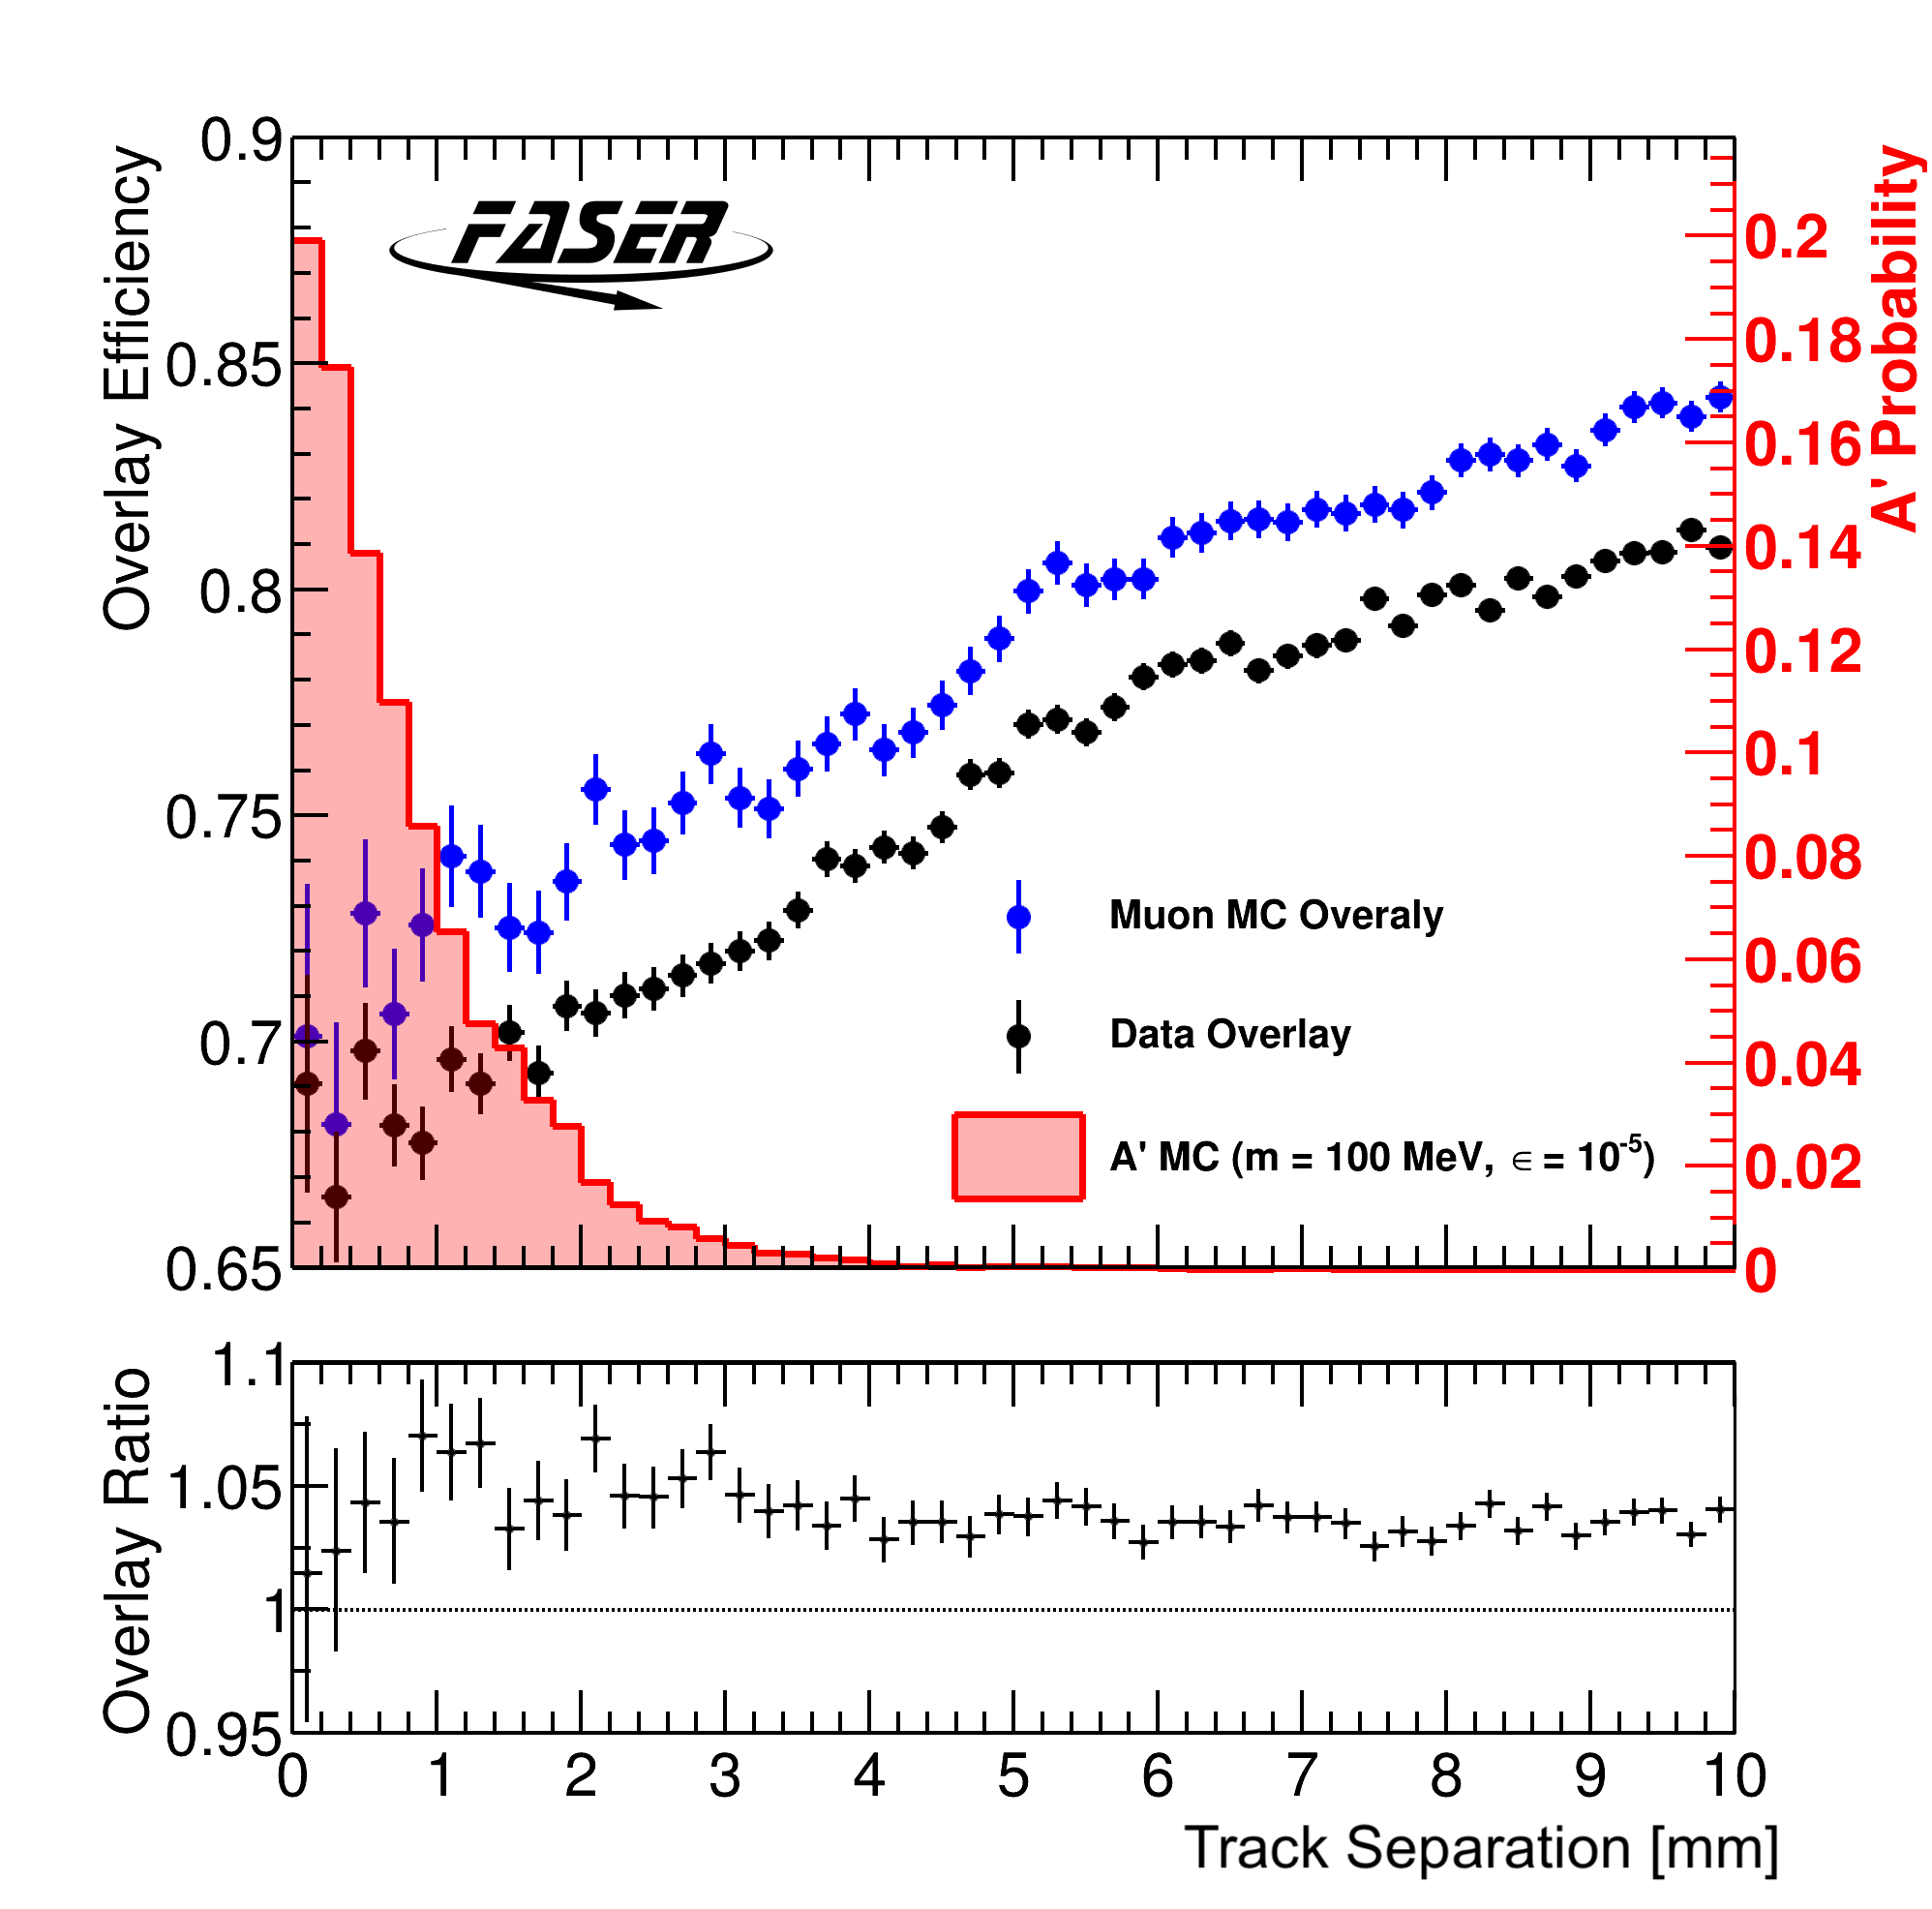
\includegraphics[width=0.7 \linewidth]{./assets/OverlayTracks.png}
		\caption{Overlay plot from \href{https://cds.cern.ch/record/2864686/plots}{Search for dark photons with the FASER detector at the LHC} }
	\end{figure}
\end{frame}

\begin{frame}{Distribution of Theta0}
	\begin{figure}
		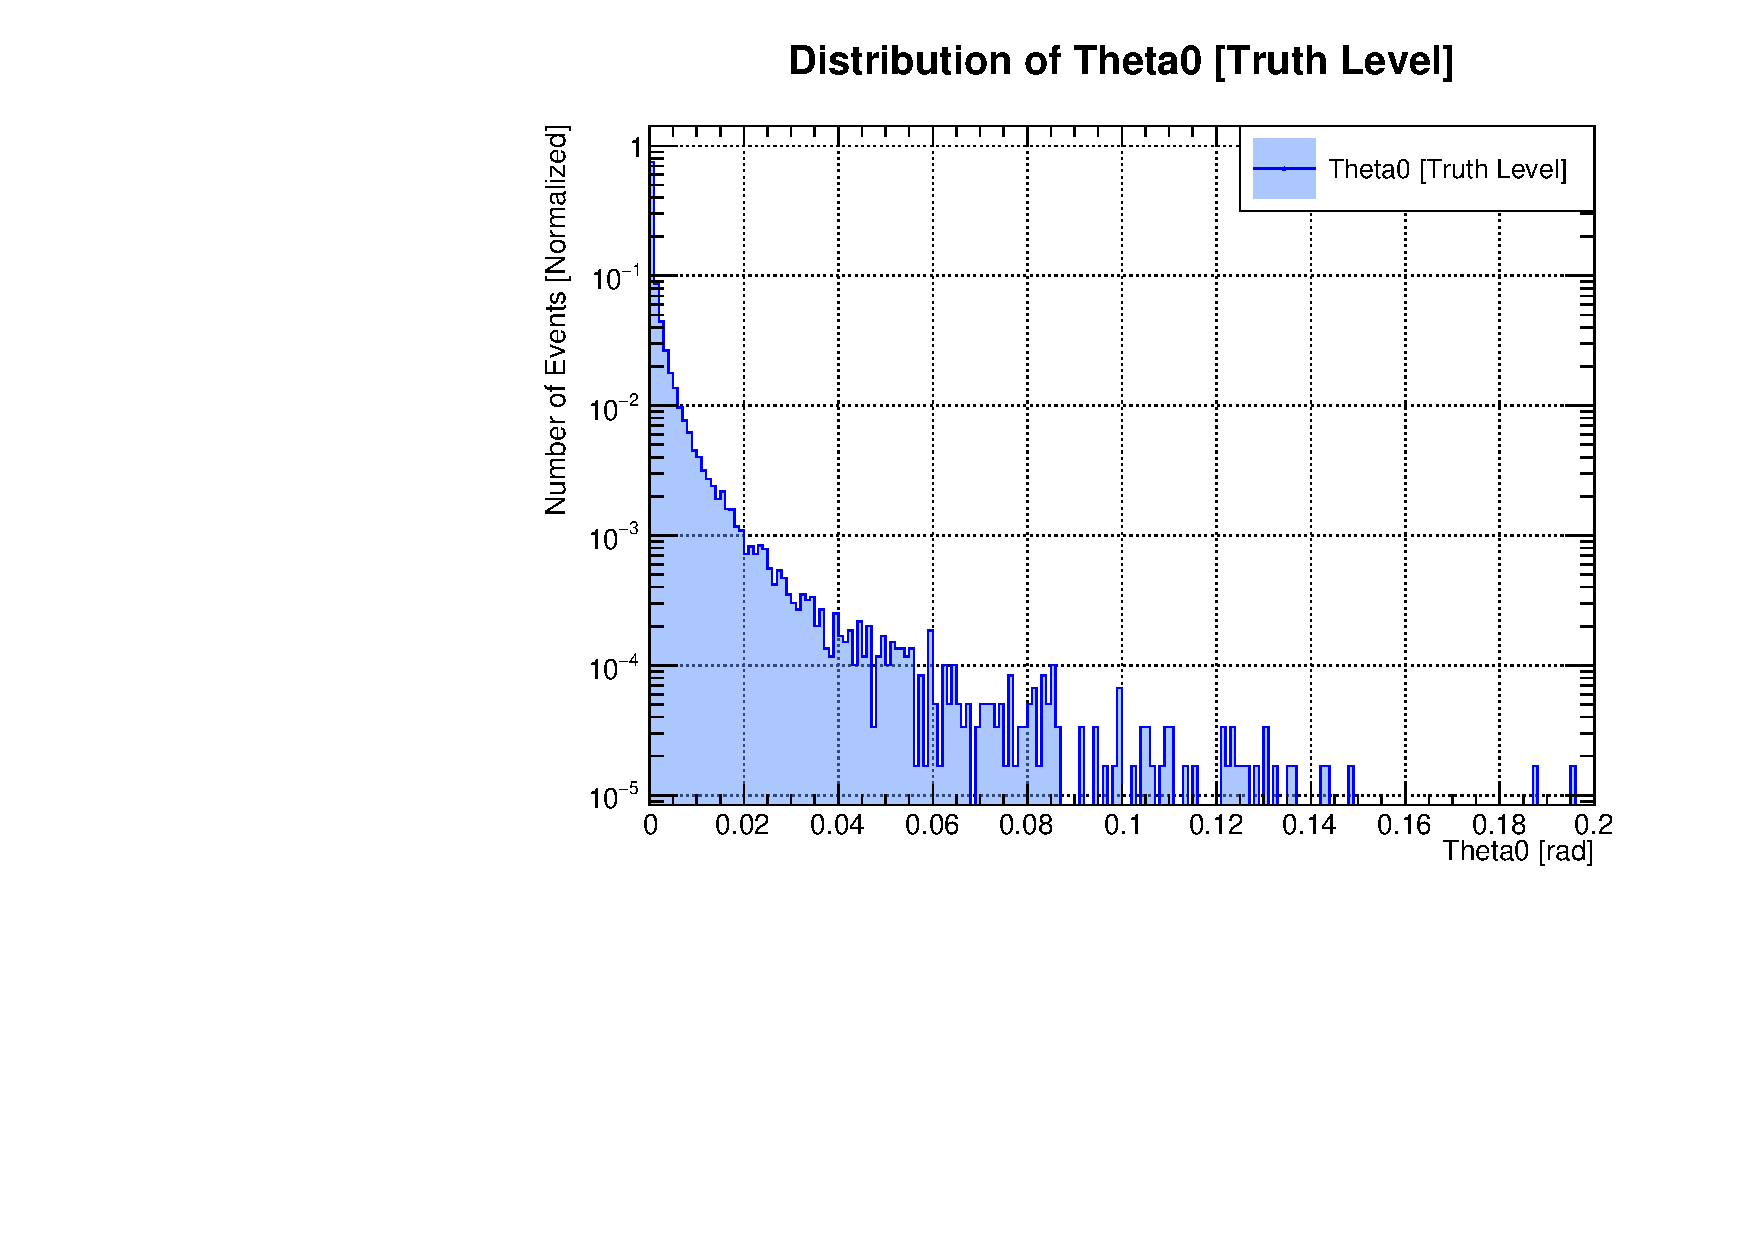
\includegraphics[width=\linewidth]{output/Theta0.pdf}
	\end{figure}
\end{frame}

\begin{frame}{Distribution of DeltaRP}
	\begin{figure}
		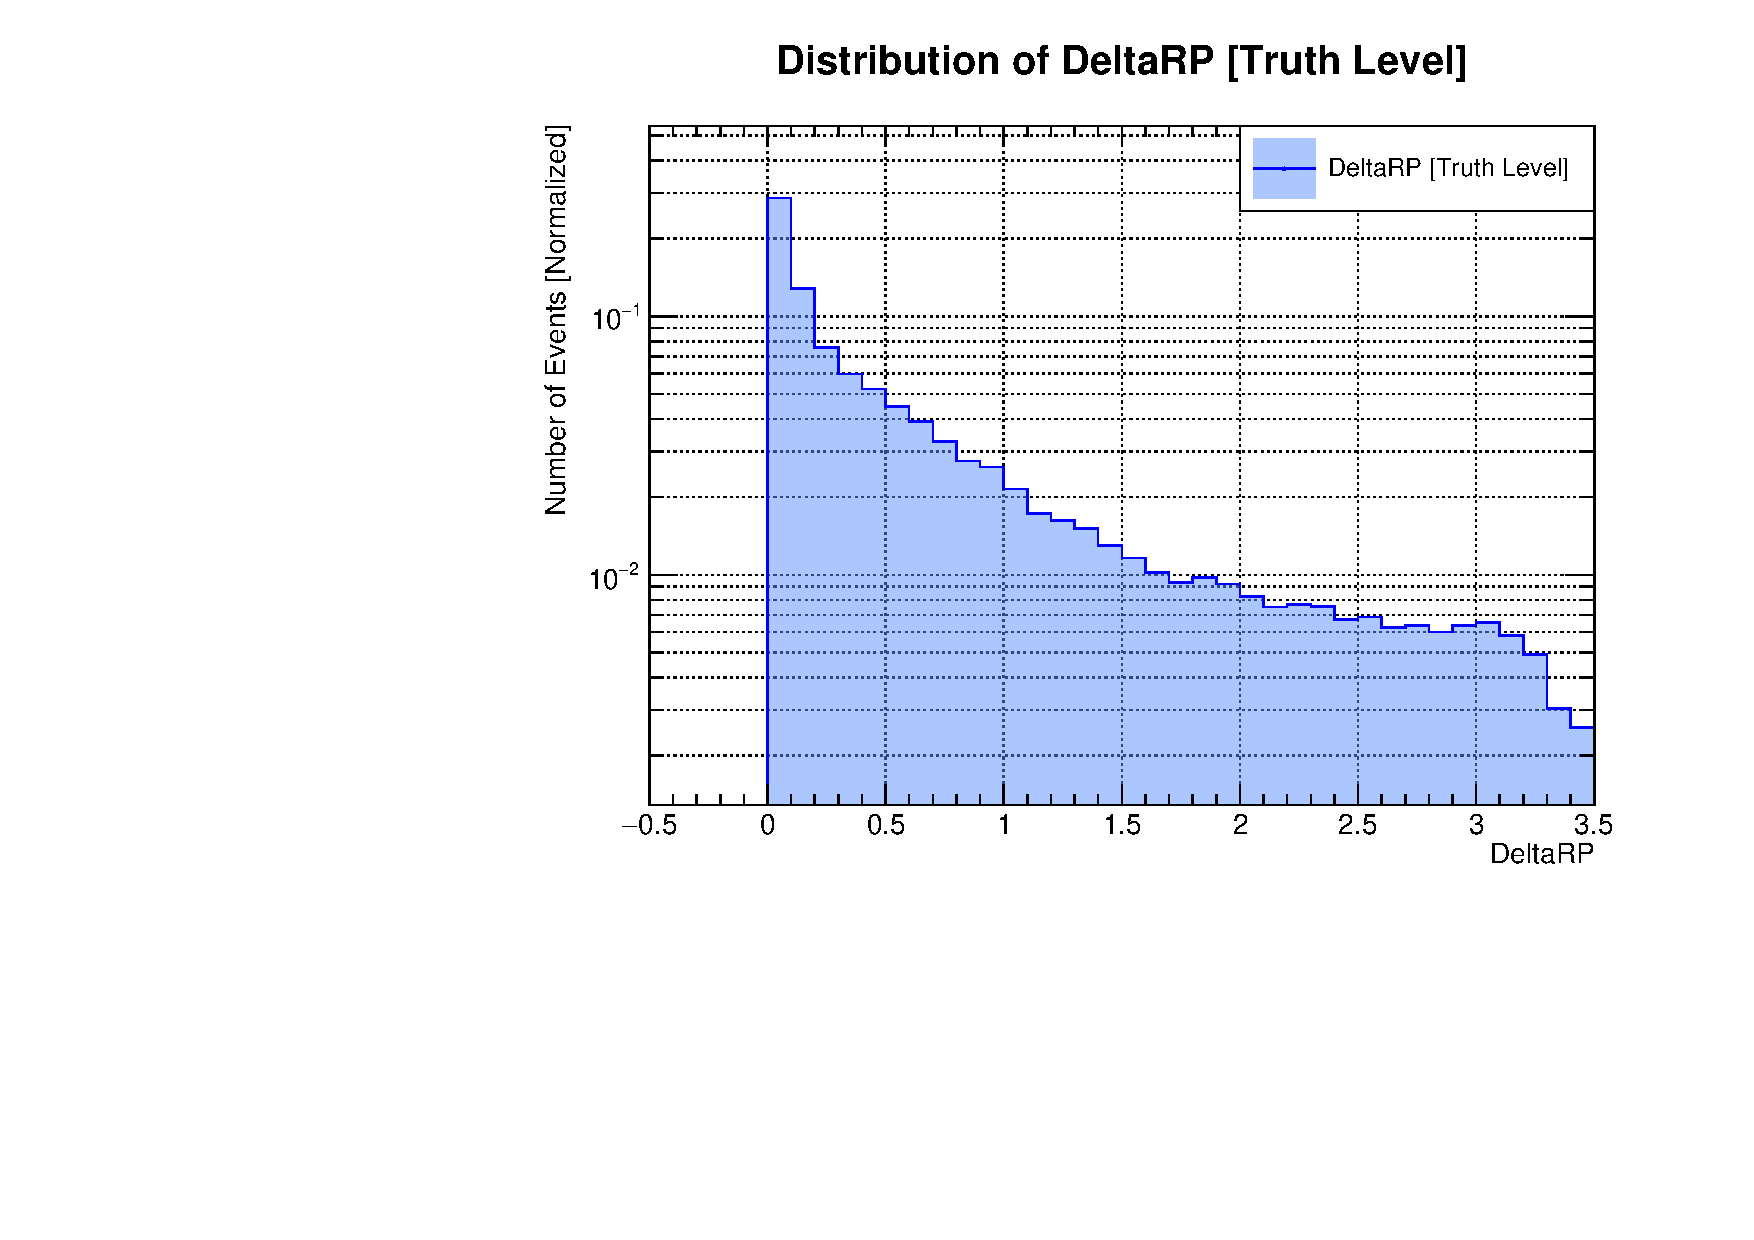
\includegraphics[width=\linewidth]{output/DeltaRP.pdf}
	\end{figure}
\end{frame}

\begin{frame}{Comments on Angle Based Separation}
	\begin{itemize}
		\item Theta0 is a variable to separate the tracks but falls off reapidly
		\item DeltaRP shows a relatively flat distribution
		% \item DeltaRP is a good variable to separate the tracks
		% \vspace{1 cm}
		\item To calculate the separation variables the MC level information is used
		\begin{itemize}
			\item Same across AL9 and CENTOS7
			\item More robust 
			\item No uncertainity from the tracking itself
		\end{itemize}
	\end{itemize}
\end{frame}
\begin{frame}{Events grouped by longTracks vs DeltaR0 }
    \begin{figure}
        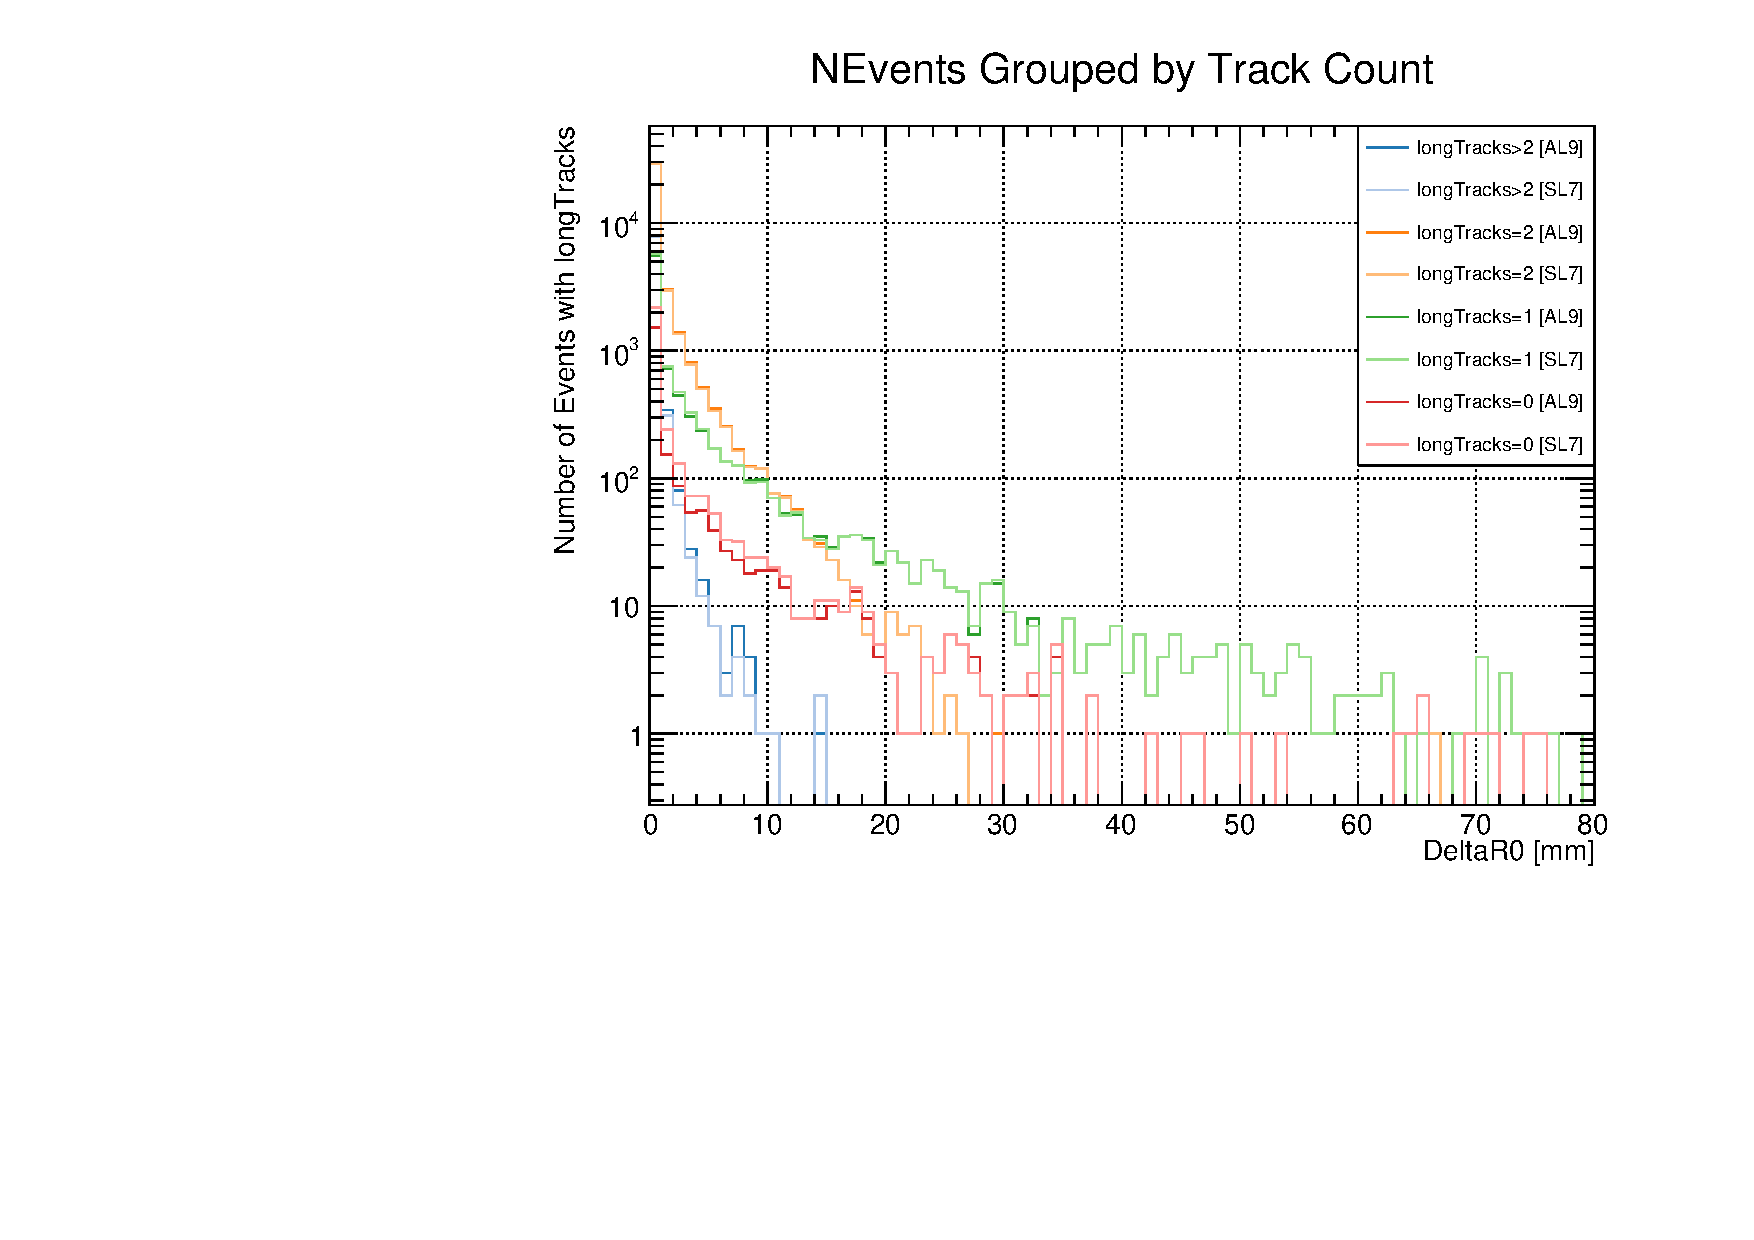
\includegraphics[width=\linewidth]{./output/Effi_DeltaR0_all.pdf}
    \end{figure}
\end{frame}

\begin{frame}{Events grouped by longTracks vs DeltaY0 [SKIP]}
    \begin{figure}
        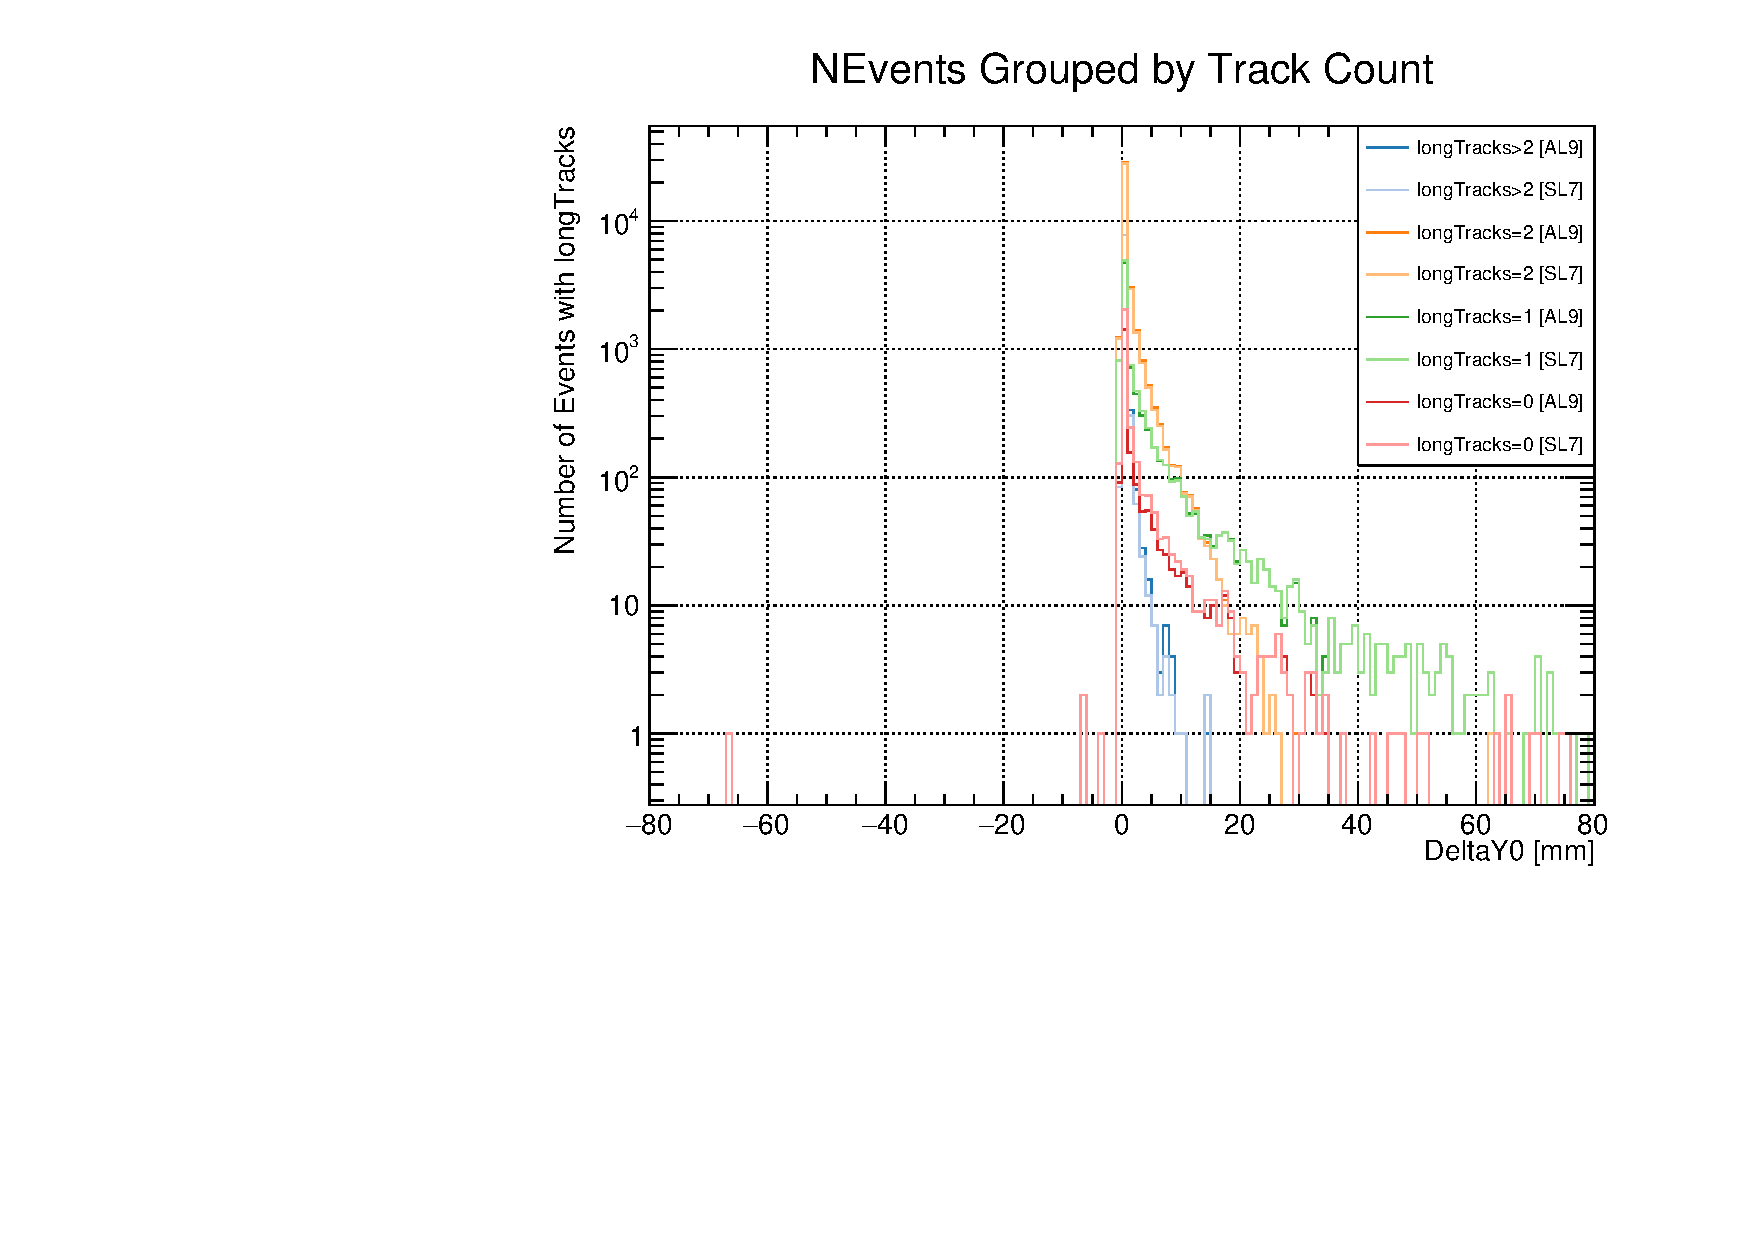
\includegraphics[width=\linewidth]{./output/Effi_DeltaY0_all.pdf}
    \end{figure}
\end{frame}

\begin{frame}{Events grouped by longTracks vs DeltaX0 [SKIP]}
    \begin{figure}
        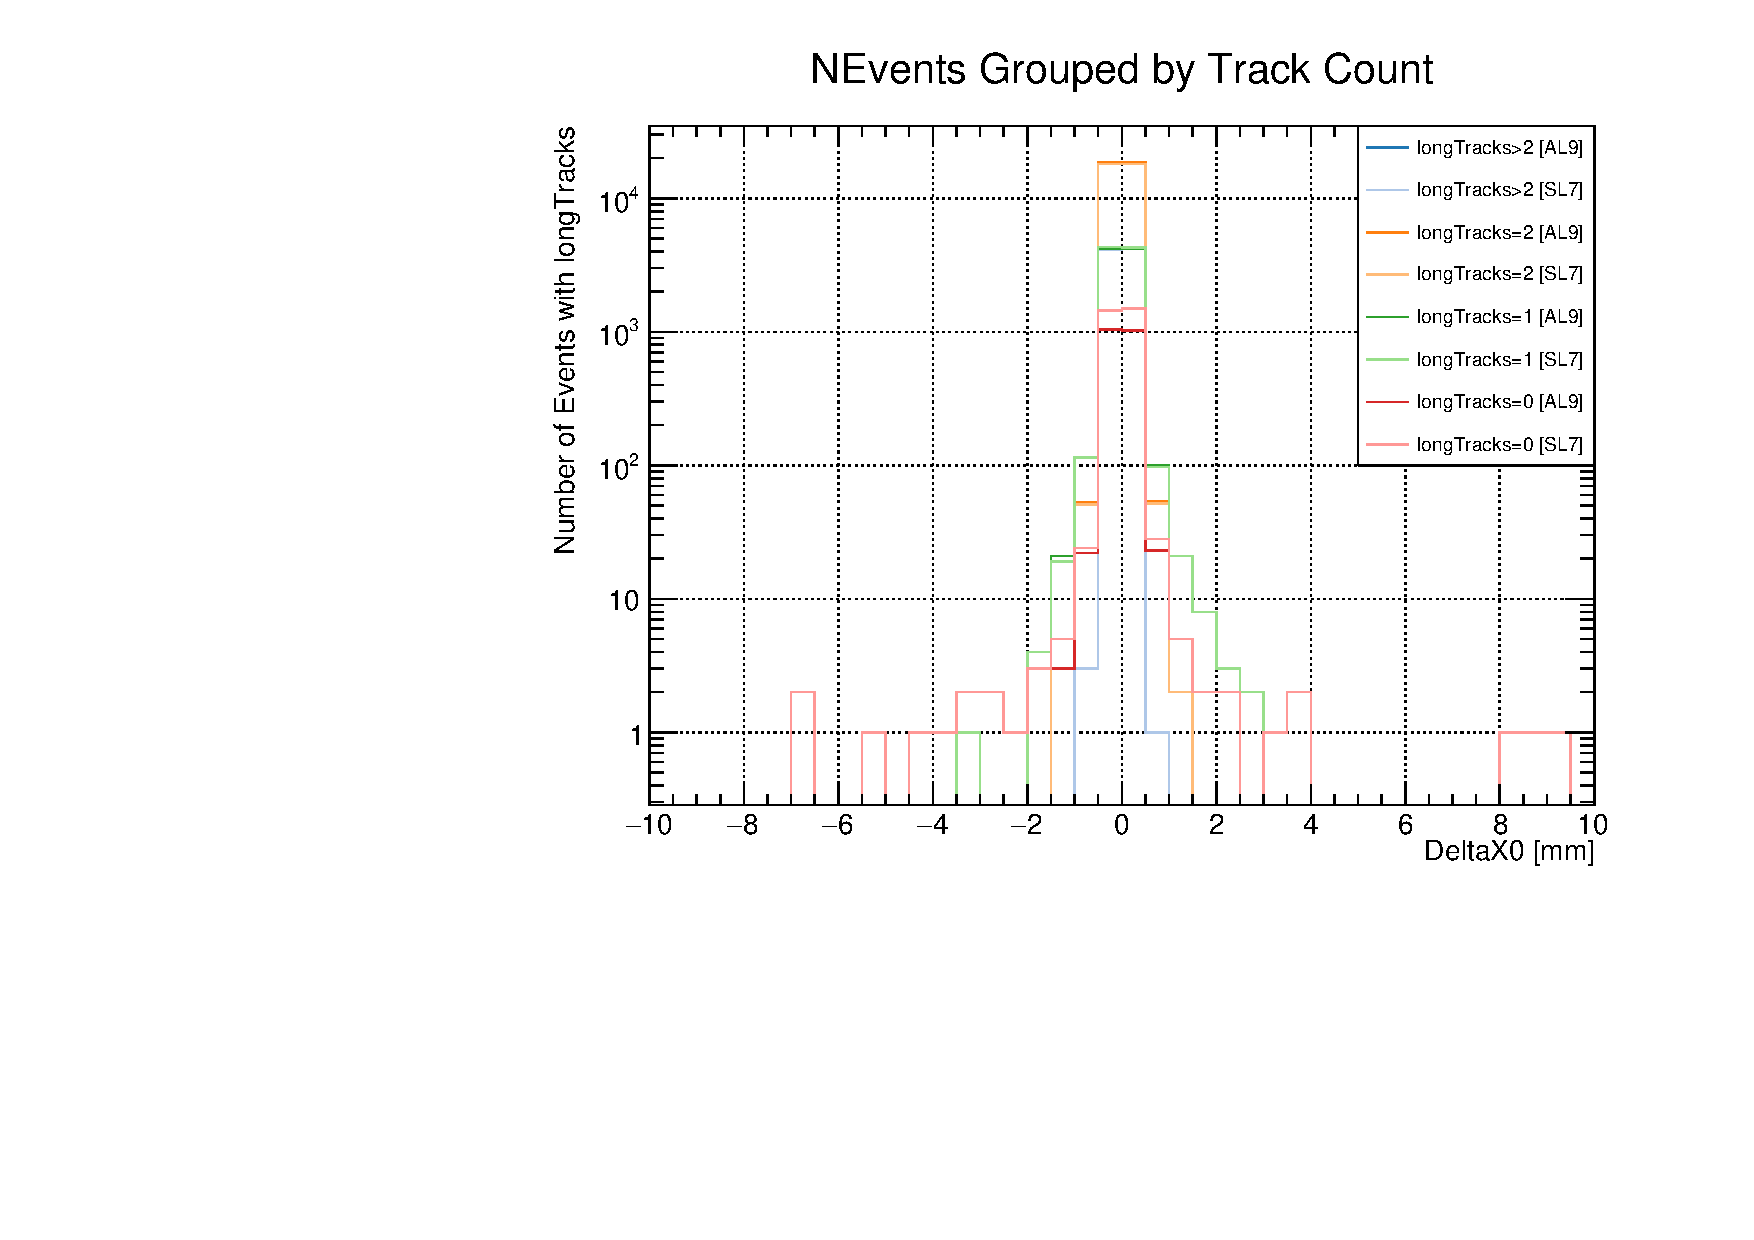
\includegraphics[width=\linewidth]{./output/Effi_DeltaX0_all.pdf}
    \end{figure}
\end{frame}

\begin{frame}{Events grouped by longTracks vs Theta0 }
    \begin{figure}
        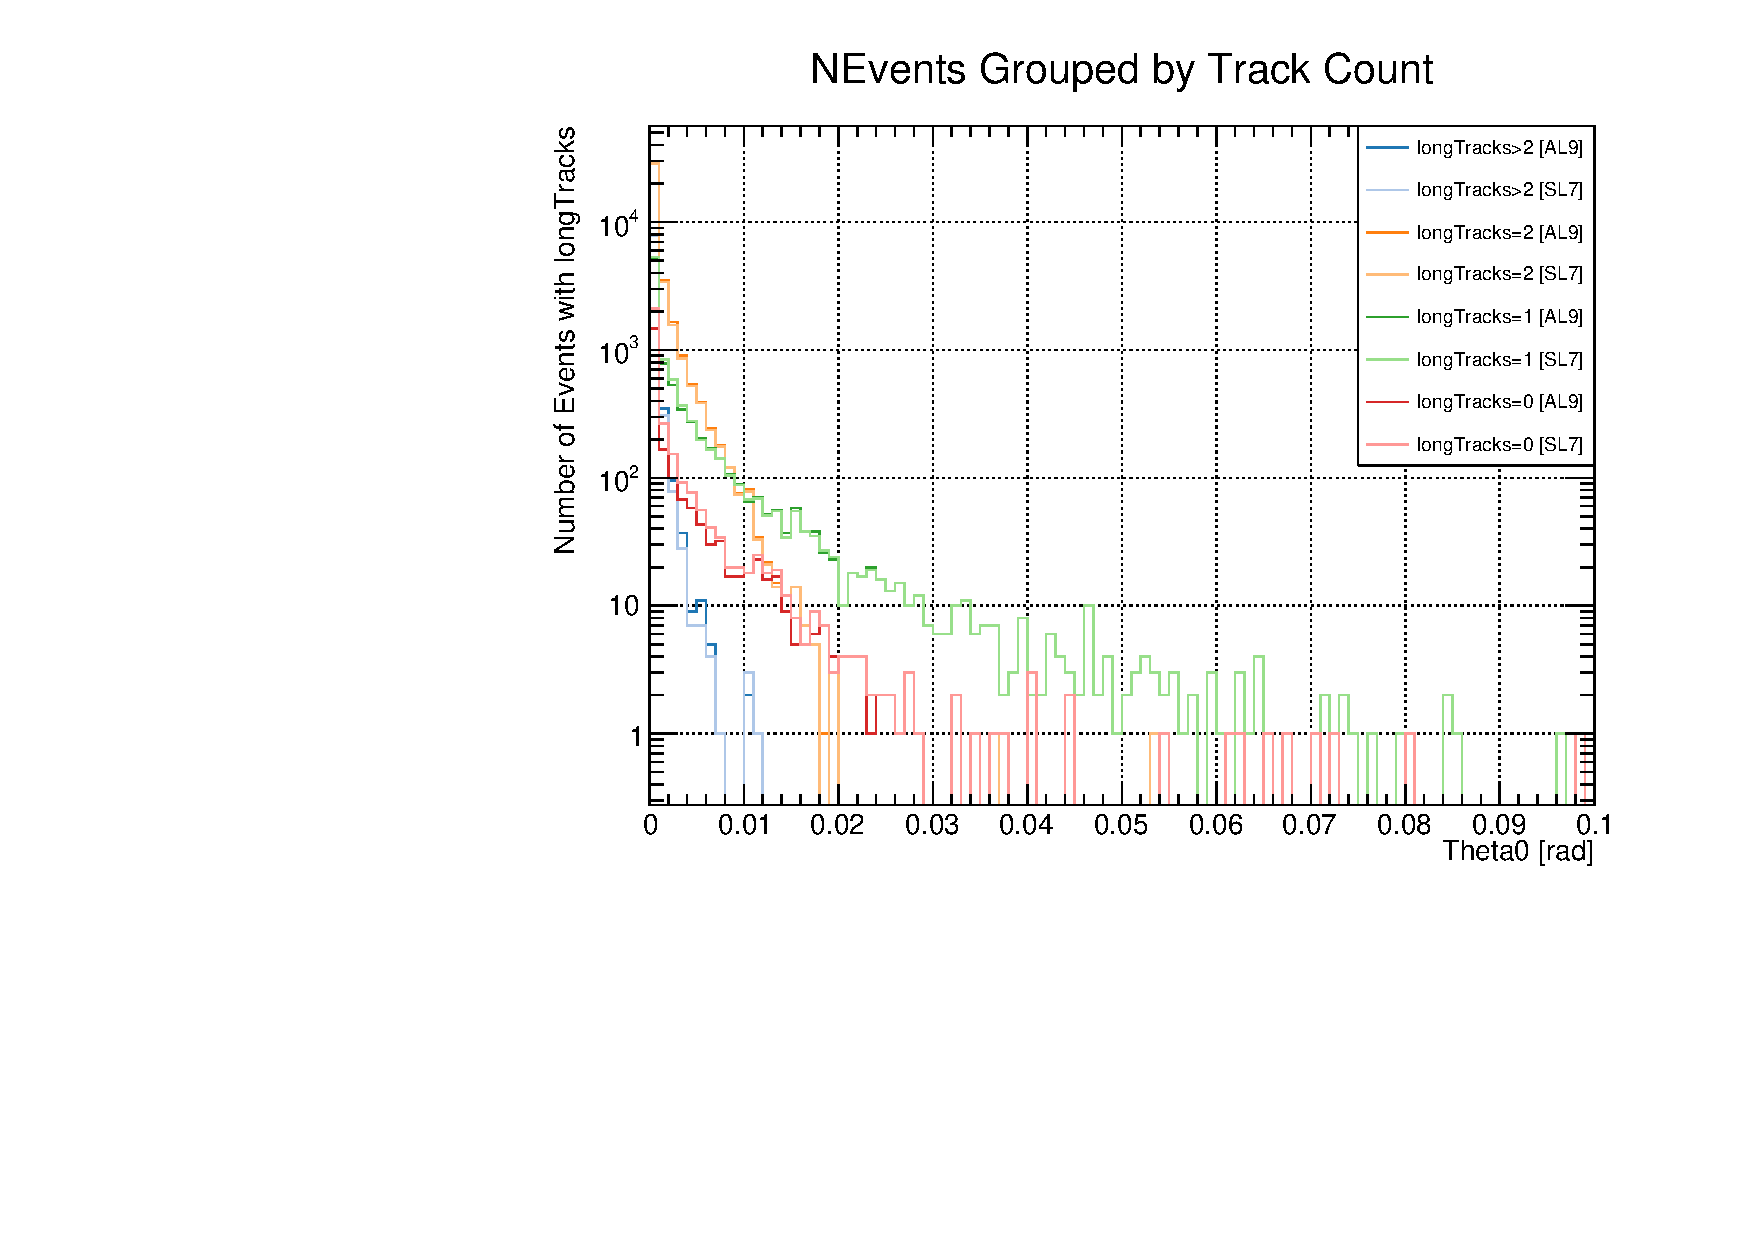
\includegraphics[width=\linewidth]{./output/Effi_Theta0_all.pdf}
    \end{figure}
\end{frame}

% \begin{frame}{Two Track Reconstruction Efficiency }
%     \begin{figure}
%         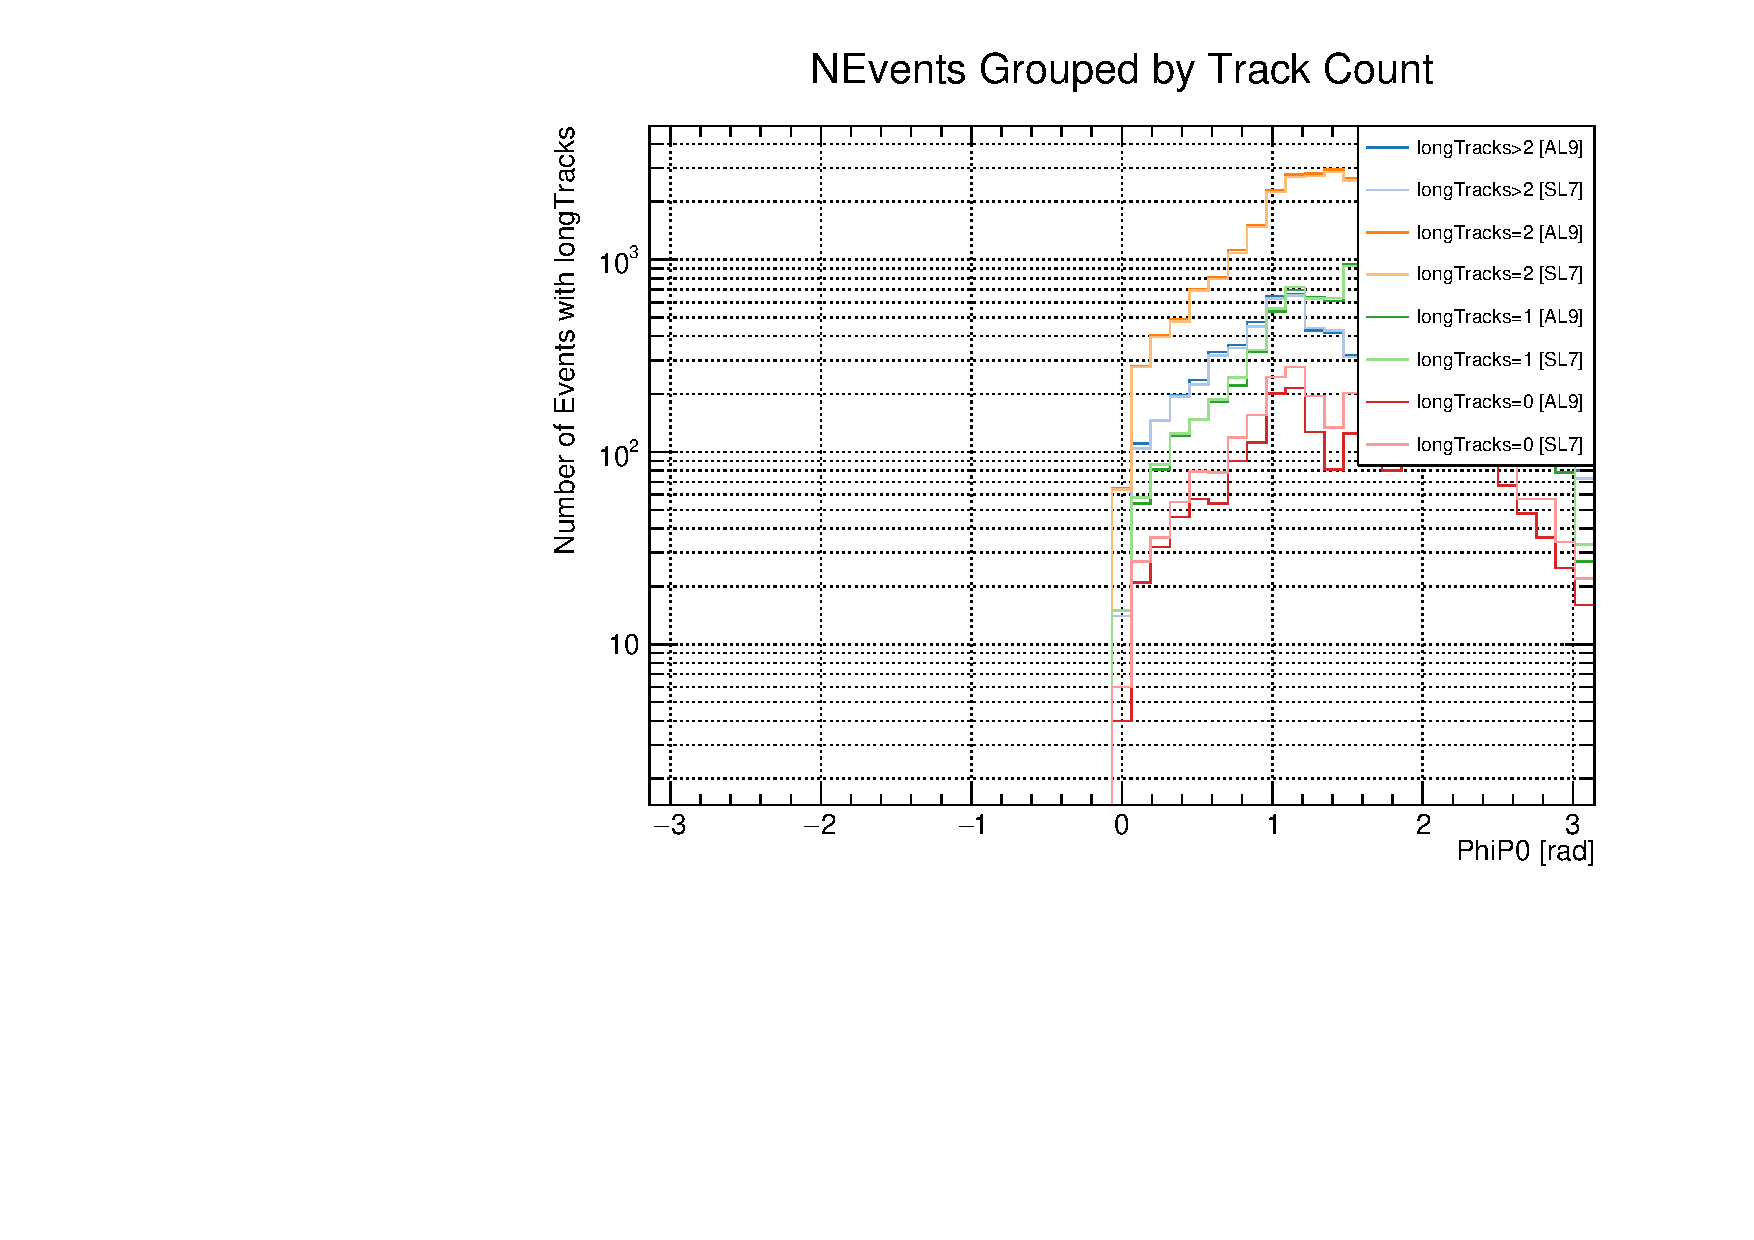
\includegraphics[width=\linewidth]{./output/Effi_PhiP0_all.pdf}
%     \end{figure}
% \end{frame}

\begin{frame}{Events grouped by longTracks vs DeltaRP}
    \begin{figure}
        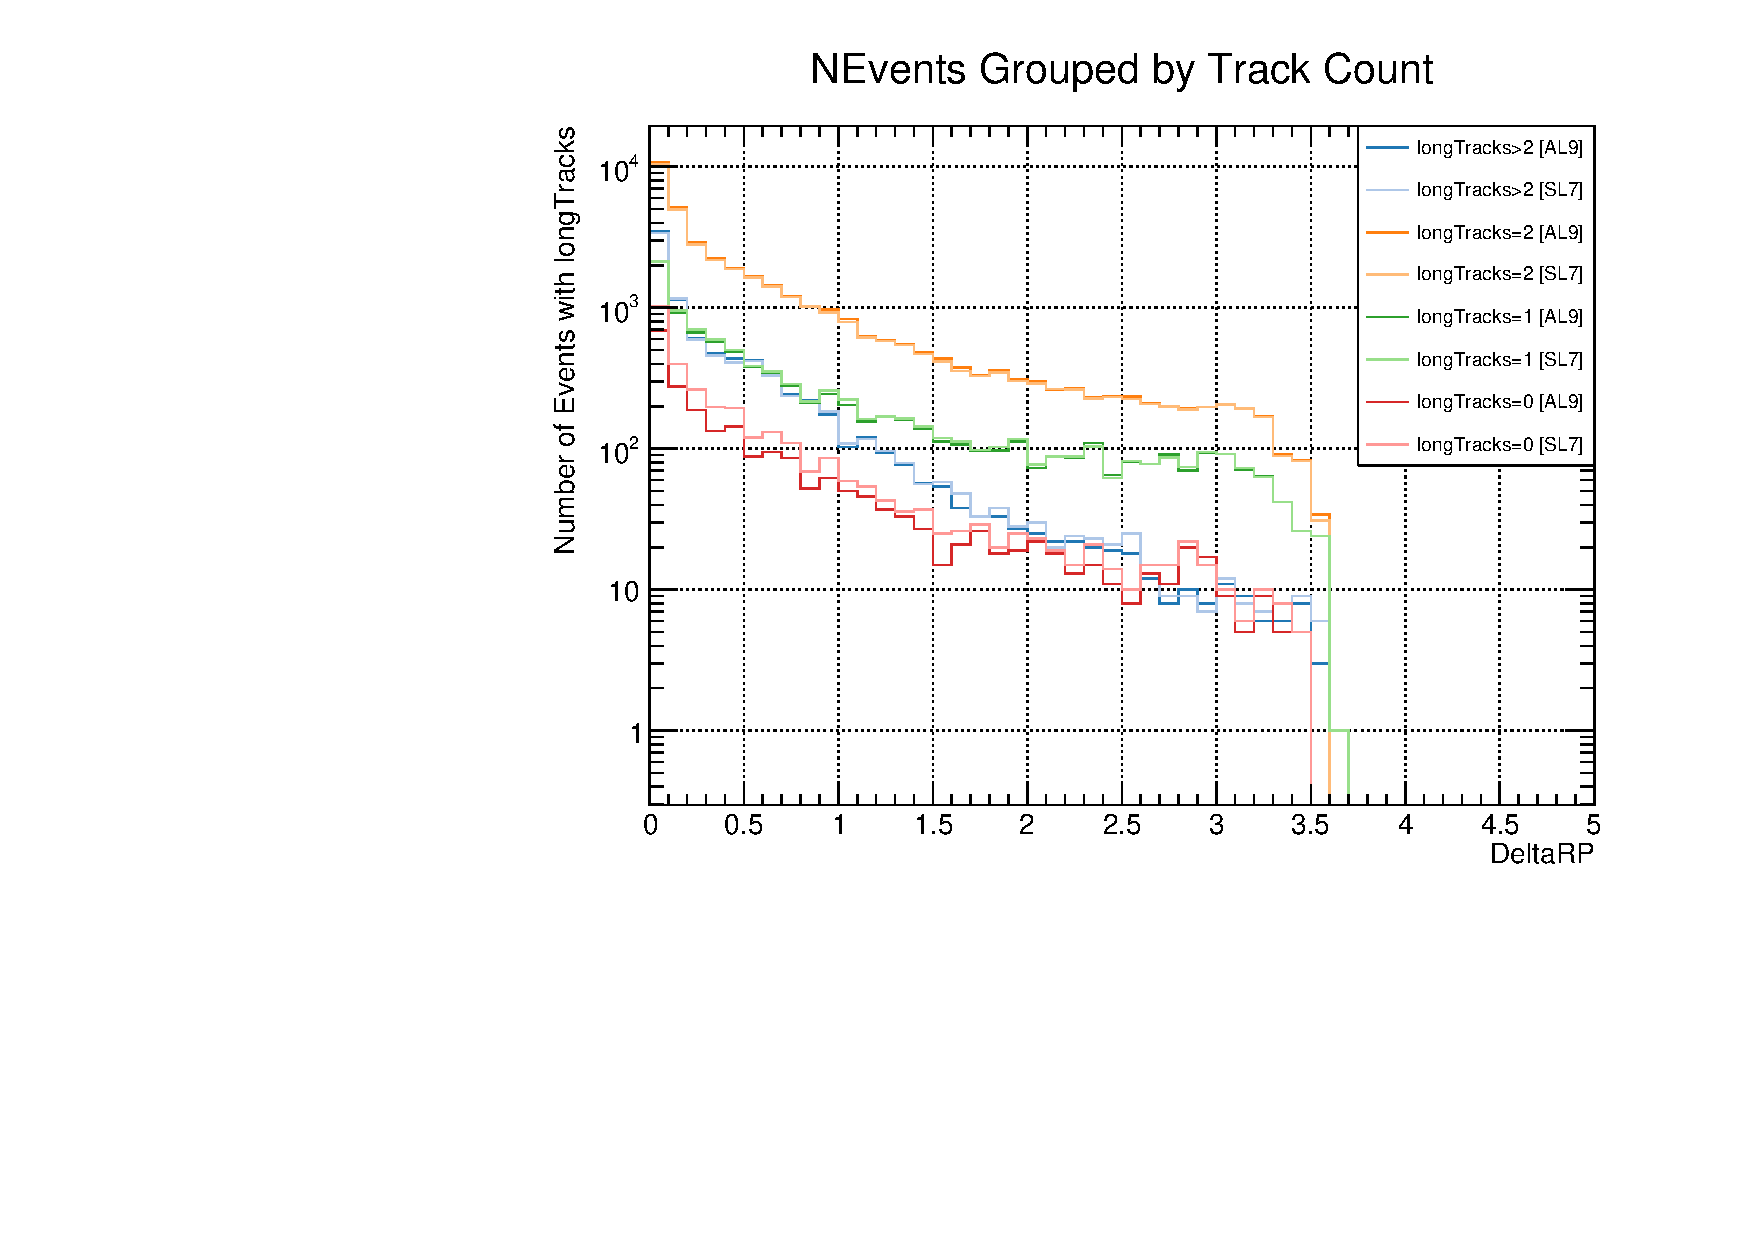
\includegraphics[width=\linewidth]{./output/Effi_DeltaRP_all.pdf}
    \end{figure}
\end{frame}

\begin{frame}{Comments on longTrack grouped Plots}
    \begin{itemize}
        \item Good agreement between ALMA9 and CENTOS7
        \item Events with $>2$ longTrack fall most rapidly [nothing past 10 mm]
        \item $=2$ longTracks decay less rapidly [nothing past 30 mm]
        \item $=1$ longTracks is relatively flat
        \item $=0$ same as above - Not sure how to interpret
        \item In the plots where longTracks $\leq$ 1 AL9 performs bad at low separation 
        \item Maybe logscale in x?
    \end{itemize}
    
\end{frame}
\begin{frame}{Definition of Efficiency Metrics}
    \textbf{In General}
	\begin{itemize}
        \item One Track Event $\implies$ NOT reconstructed
        \item Two Track event + Opposite charges $\implies$ reconstructed 
        \item More than two track $\implies$ complicated
    \end{itemize}
    \vspace{1 cm}
    \textbf{Some Possible Eff. Metrics}
    \begin{itemize}
        \item Number of Events with $\geq$ 2 longTracks [good proxy]
        \item (Can add charge identification to above but not necessary)
        \item MC Based Effi. [matching reconstructed to truth level data]
    \end{itemize}
\end{frame}

\begin{frame}{Definition of Fiducial}
    Before we define the efficiency we need to account for the detector acceptance by requiring the particle to be Fiducial.

		\textbf{Based on reconstructed data [Adapted from Sinead]}
		\begin{itemize}
			\item Requires $longTracks == 2$ 
			\item $Track\_r\_atMaxRadius < 100$
			\item $t\_st\{1,2,3\}\_r < 100$
 		\end{itemize}
		\textbf{Based on truth level data }
		\begin{itemize}
			\item $truthd0\_r [\{1,2,3\}] < 100$
			\item $truthd1\_r [\{1,2,3\}] < 100$
			\item Does not need the 2track cut while maintaining that particles of interest were Fiducial, While also being independent of ALMA9 or CENTOS7
	
		\end{itemize}

        \textbf{Note:}
        \begin{itemize}
		\item Where are NaNs coming from at the truth-level?
	    \end{itemize}	
\end{frame}

\begin{frame}{How do Fiducial Cuts perform?}
    \begin{table}[h!]
        \centering
        \small
        \begin{tabular}{|l|c|c|c|c|}
        \hline
        \textbf{Selection Step} & \textbf{Pass} & \textbf{All} & \textbf{Effi. (\%)} & \textbf{Cum. Effi. (\%)} \\ \hline
        2LongTracks              & 37807        & 60000       & 63.01                   & 63.01                              \\ \hline
        Opposite Charge          & 32427        & 37807       & 85.77                   & 54.04                              \\ \hline
        MaxRadius $<$ 100        & 31489    & 32427       & 97.11                   & 52.48                              \\ \hline
        $t\_st1\_r < 100$        & 31471        & 31489       & 99.94                   & 52.45                              \\ \hline
        $t\_st2\_r < 100$        & 31458        & 31471       & 99.96                   & 52.43                              \\ \hline
        $t\_st3\_r < 100$        & 31383        & 31458       & 99.76                   & 52.31                              \\ \hline
        \end{tabular}
        \caption{Efficiencies and cumulative efficiencies at various selection steps. [ALMA9]}
        \label{table:efficiency}
    \end{table}
    \vspace{-0.5cm}
    \begin{table}[h!]
        \centering
        \small
        \begin{tabular}{|l|c|c|c|c|}
        \hline
        \textbf{Selection Step} & \textbf{Pass} & \textbf{All} & \textbf{Effi. (\%)} & \textbf{Cum. Effi. (\%)} \\ \hline
        2LongTracks              & 36746        & 60000       & 61.24                   & 61.24                              \\ \hline
        Opposite Charge          & 30375        & 36746       & 82.66                   & 50.62                              \\ \hline
        MaxRadius $<$ 100 & 29520    & 30375       & 97.19                   & 49.20                              \\ \hline
        $t\_st1\_r < 100$        & 29498        & 29520       & 99.93                   & 49.16                              \\ \hline
        $t\_st2\_r < 100$        & 29491        & 29498       & 99.98                   & 49.15                              \\ \hline
        $t\_st3\_r < 100$        & 29415        & 29491       & 99.74                   & 49.03                              \\ \hline
        \end{tabular}
        \caption{Efficiencies and cumulative efficiencies at various selection steps.[CENTOS7]}
        \label{table:efficiency_updated}
        \end{table}        
        \vspace{-0.5cm}
        \begin{itemize}
            \item ALMA9 performs better over most of the cuts. 
            \item Using this fiducial cuts throws out 50\% of the data.
        \end{itemize}        
\end{frame}

\begin{frame}{Cuts. Contd.}
    \begin{table}[h!]
        \centering
        \small
        \begin{tabular}{|l|c|c|c|c|}
        \hline
        \textbf{Selection Step} & \textbf{Pass} & \textbf{All} & \textbf{Effi. (\%)} & \textbf{Cum. Effi. (\%)} \\ \hline
        truthd\{0,1\}\_st1\_r $<$ 100    & 59634        & 60000       & 99.39                   & 99.39                              \\ \hline
        truthd\{0,1\}\_st2\_r $<$ 100   & 58429        & 59634       & 97.98                   & 97.38                              \\ \hline
        truthd\{0,1\}\_st3\_r $<$ 100   & 56703        & 58429       & 97.05                   & 94.50                              \\ \hline
        \end{tabular}
        \caption{Efficiencies and cumulative efficiencies for truth-level selection steps. [same for ALMA9/CENTOS7]}
        \label{table:truth_efficiency}
    \end{table}
        truthd\_st1\_r = \\
        \hspace{0.5cm}sqrt( pow(truthd0\_x[1],2) + pow(truthd0\_y[1],2) ) $>$ 100 \&\& \\
        \hspace{0.5cm}sqrt( pow(truthd1\_x[1],2) + pow(truthd1\_y[1],2) )
\end{frame}

\begin{frame}{Efficiency Definition}
    \begin{itemize}
        \item Remove acceptance based on fiducial cuts at truth level
        \item Define Efficiency as the fraction of events with more than 2 reconstructed longTracks divided by the total number of events. 
        \[ \text{Efficiency} = \frac{\text{NEvents}({\geq 2 \text{longTracks}})}{\text{NEvents}({\text{Total}})} \]
    \end{itemize}
\end{frame}

\begin{frame}{$>=2$ Track Efficiency as a function of DeltaR0}
    \begin{figure}
        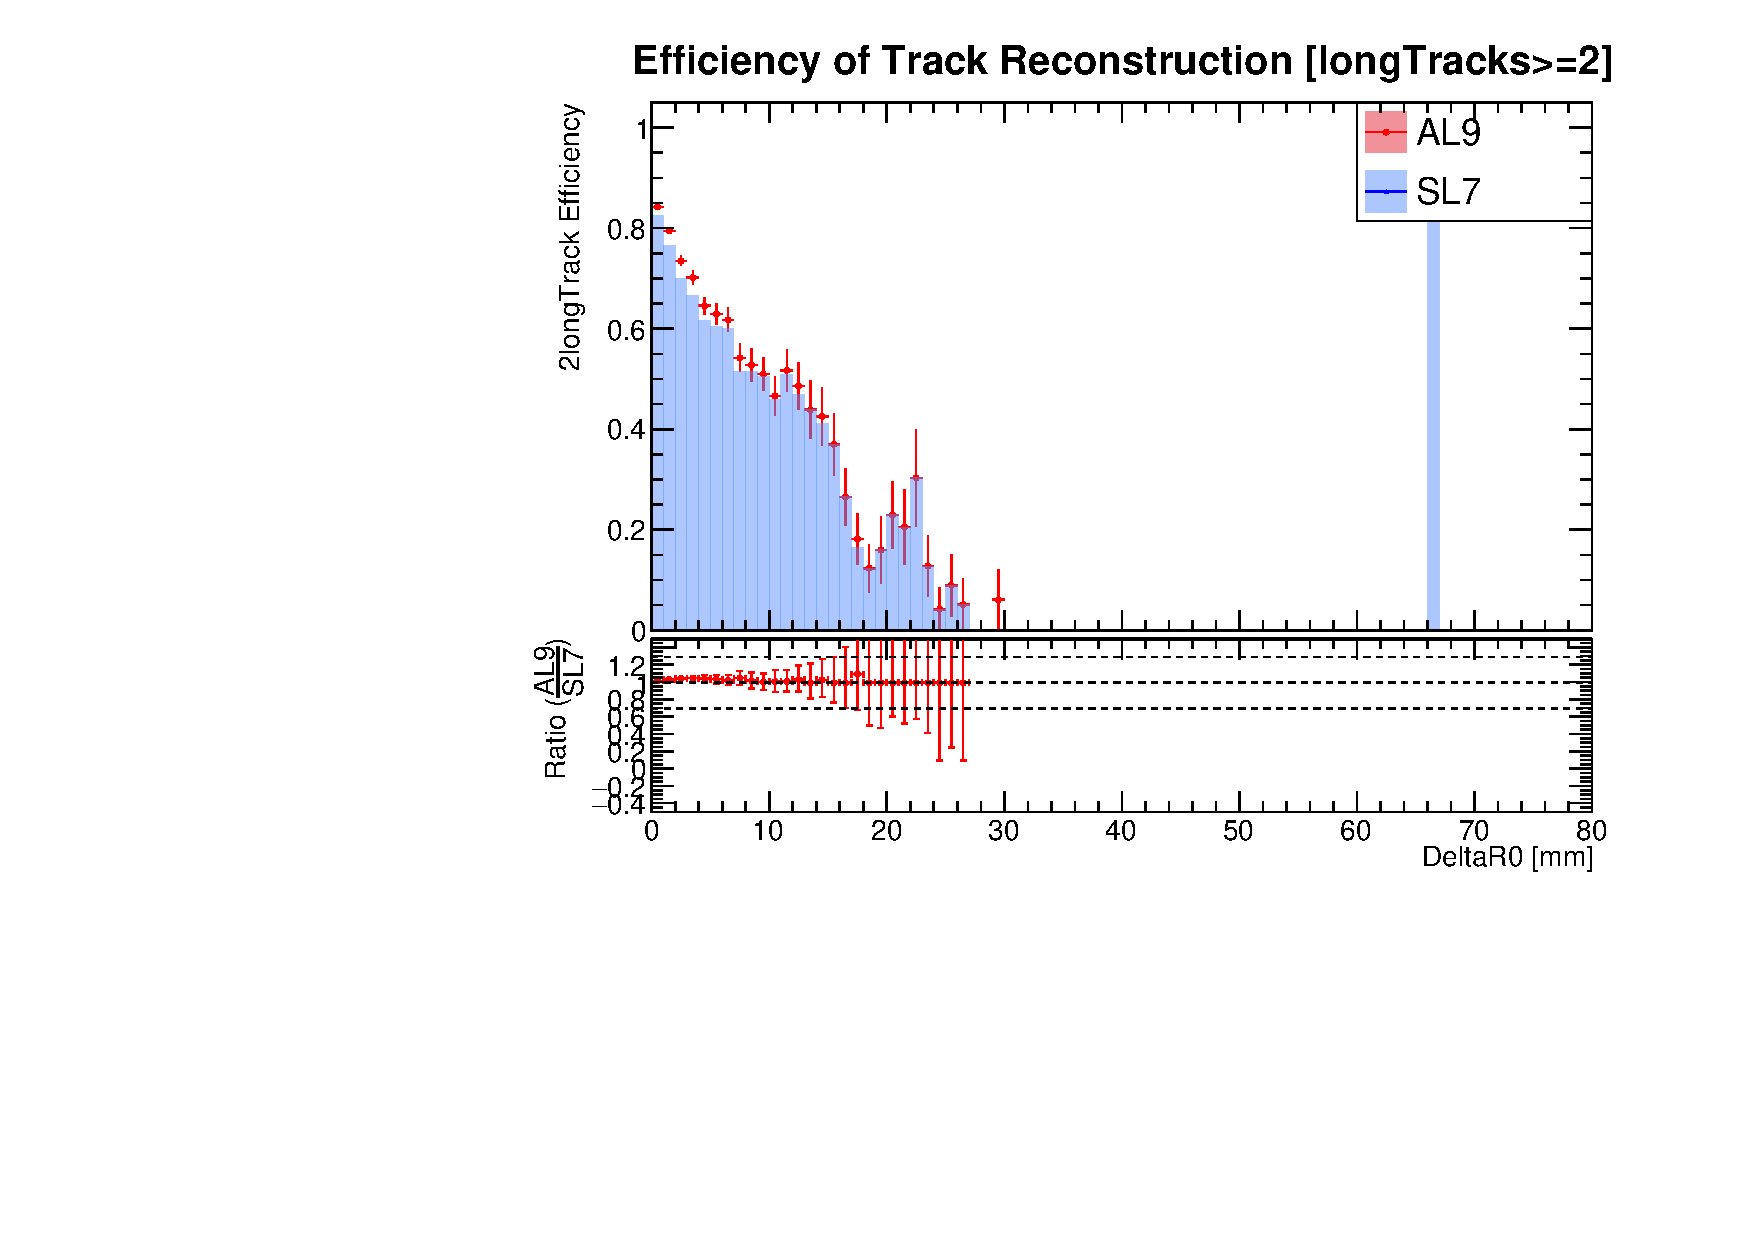
\includegraphics[width=\linewidth]{./output/Effi_greq2_DeltaR0.pdf}
    \end{figure}
\end{frame}
\begin{frame}{$>=2$ Track Efficiency as a function of DeltaX0 [SKIP]}
    \begin{figure}
        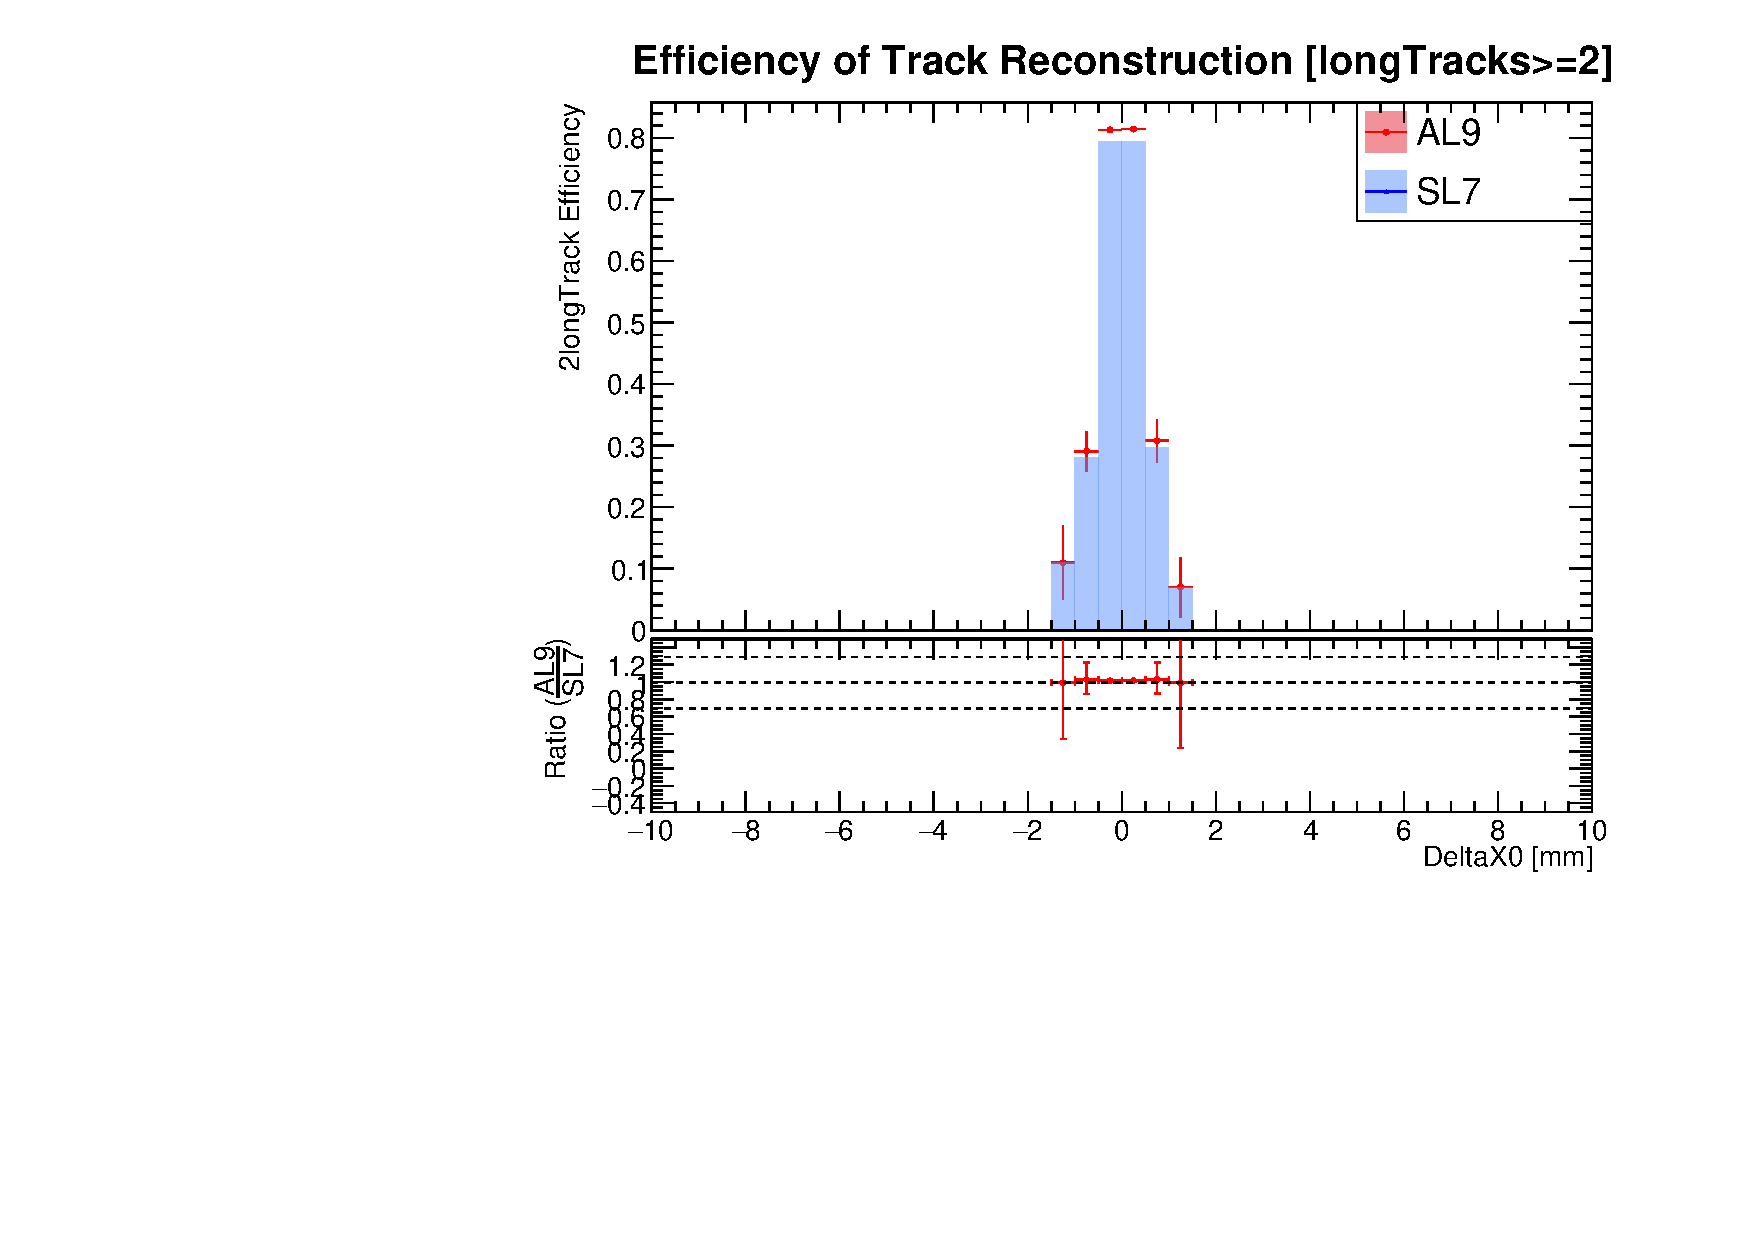
\includegraphics[width=\linewidth]{./output/Effi_greq2_DeltaX0.pdf}

    \end{figure}
\end{frame}
\begin{frame}{$>=2$ Track Efficiency as a function of DeltaY0 [SKIP]}
    \begin{figure}
        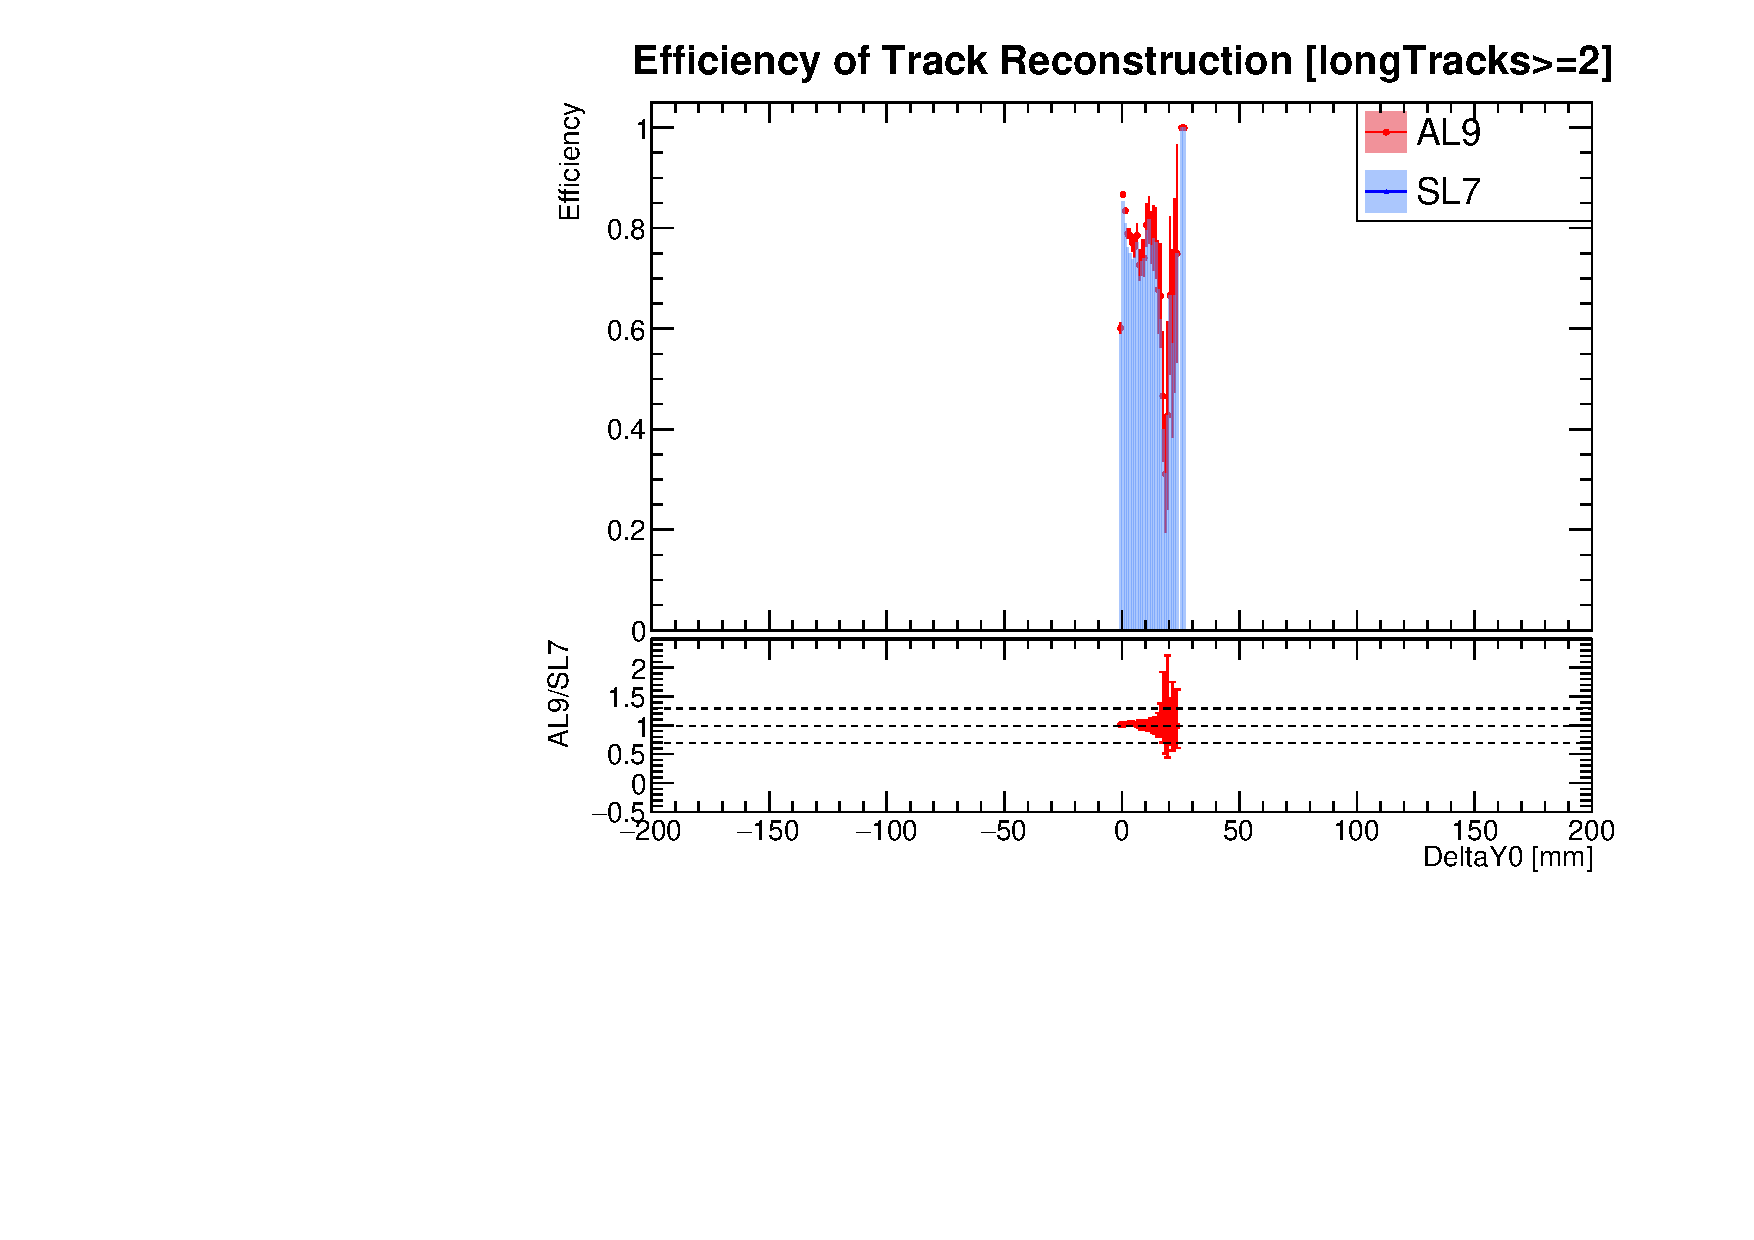
\includegraphics[width=\linewidth]{./output/Effi_greq2_DeltaY0.pdf}
    \end{figure}
\end{frame}
\begin{frame}{$>=2$ Track Efficiency as a function of Theta0}
    \begin{figure}
        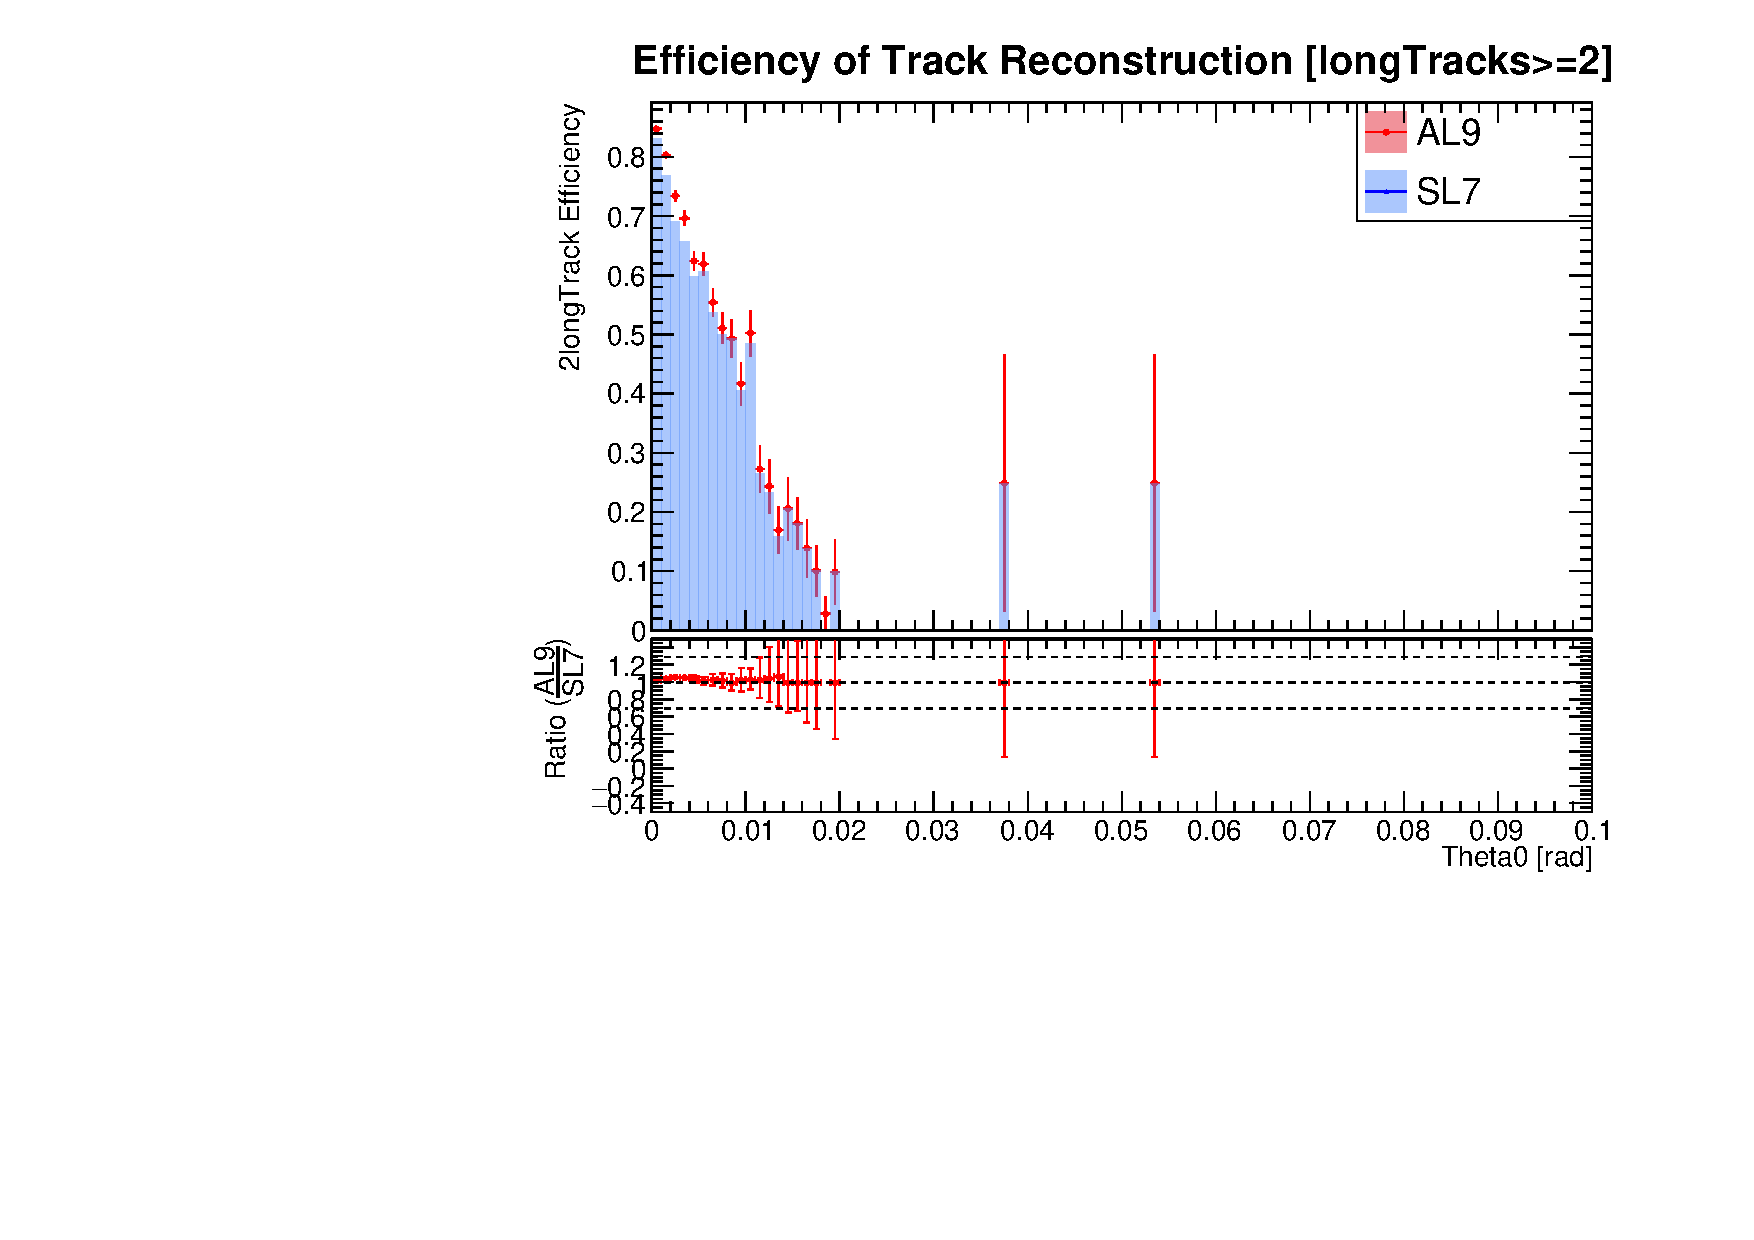
\includegraphics[width=\linewidth]{./output/Effi_greq2_Theta0.pdf}
    \end{figure}
\end{frame}
\begin{frame}{$>=2$ Track Efficiency as a function of DeltaRP}
    \begin{figure}
        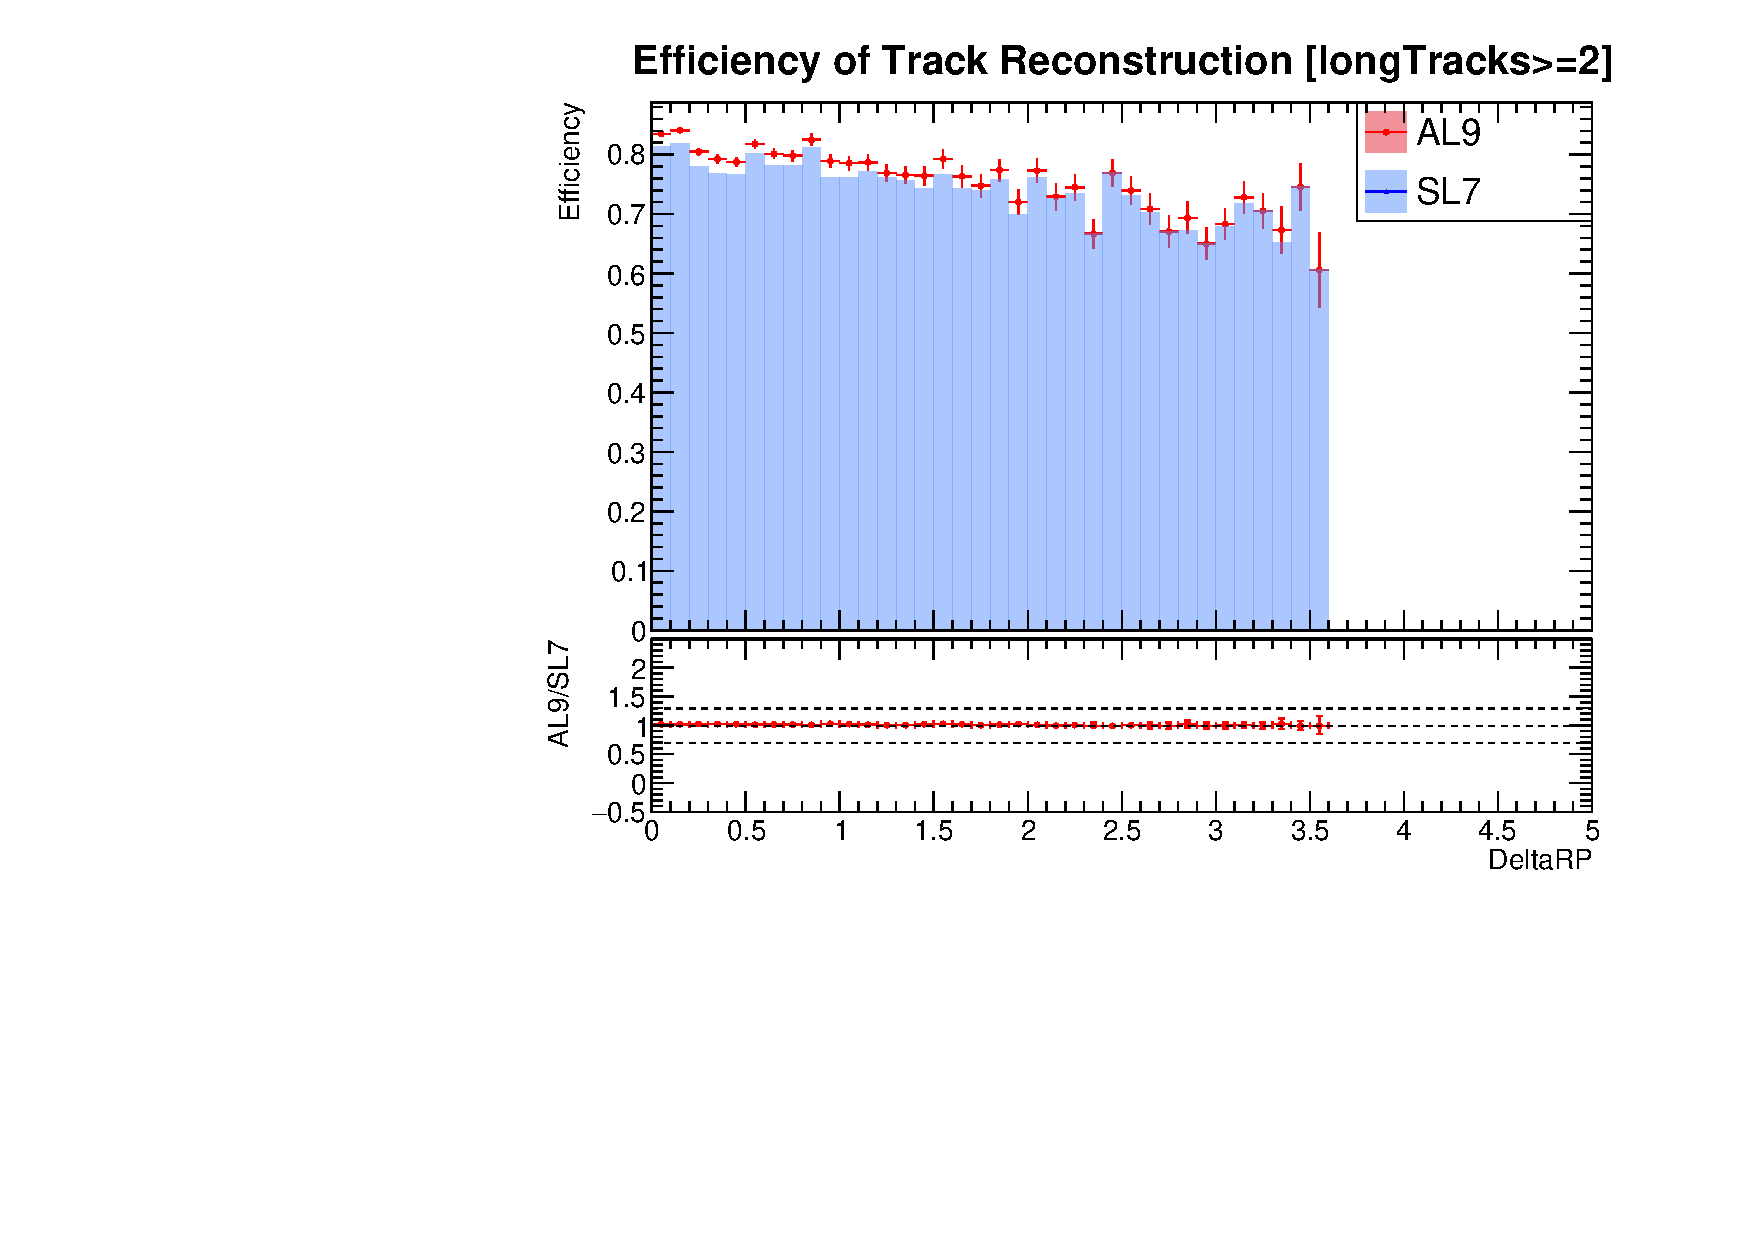
\includegraphics[width=\linewidth]{./output/Effi_greq2_DeltaRP.pdf}
    \end{figure}
\end{frame}

\begin{frame}{Comments on $>$2Track Efficiency}
    \begin{itemize}
        \item Good agreement between ALMA9 and CENTOS7
        \item Minor bump at very low separation ($\approx$ 2-6 mm) for ALMA9 
        \item Error Bars too significant to say anything about large separation
    \end{itemize}
\end{frame}

\begin{frame}{Alternate Efficiency Definition}
    \begin{itemize}
        \item Remove acceptance based on fiducial cuts at truth level
        \item Define Efficiency as the fraction of events with exactly 2 reconstructed longTracks divided by the total number of events. 
        \[ \text{Efficiency} = \frac{\text{NEvents}({= 2 \text{longTracks}})}{\text{NEvents}({\text{Total}})} \]
    \end{itemize}
\end{frame}

\begin{frame}{2 Track Efficiency as a function of DeltaR0}
    \begin{figure}
        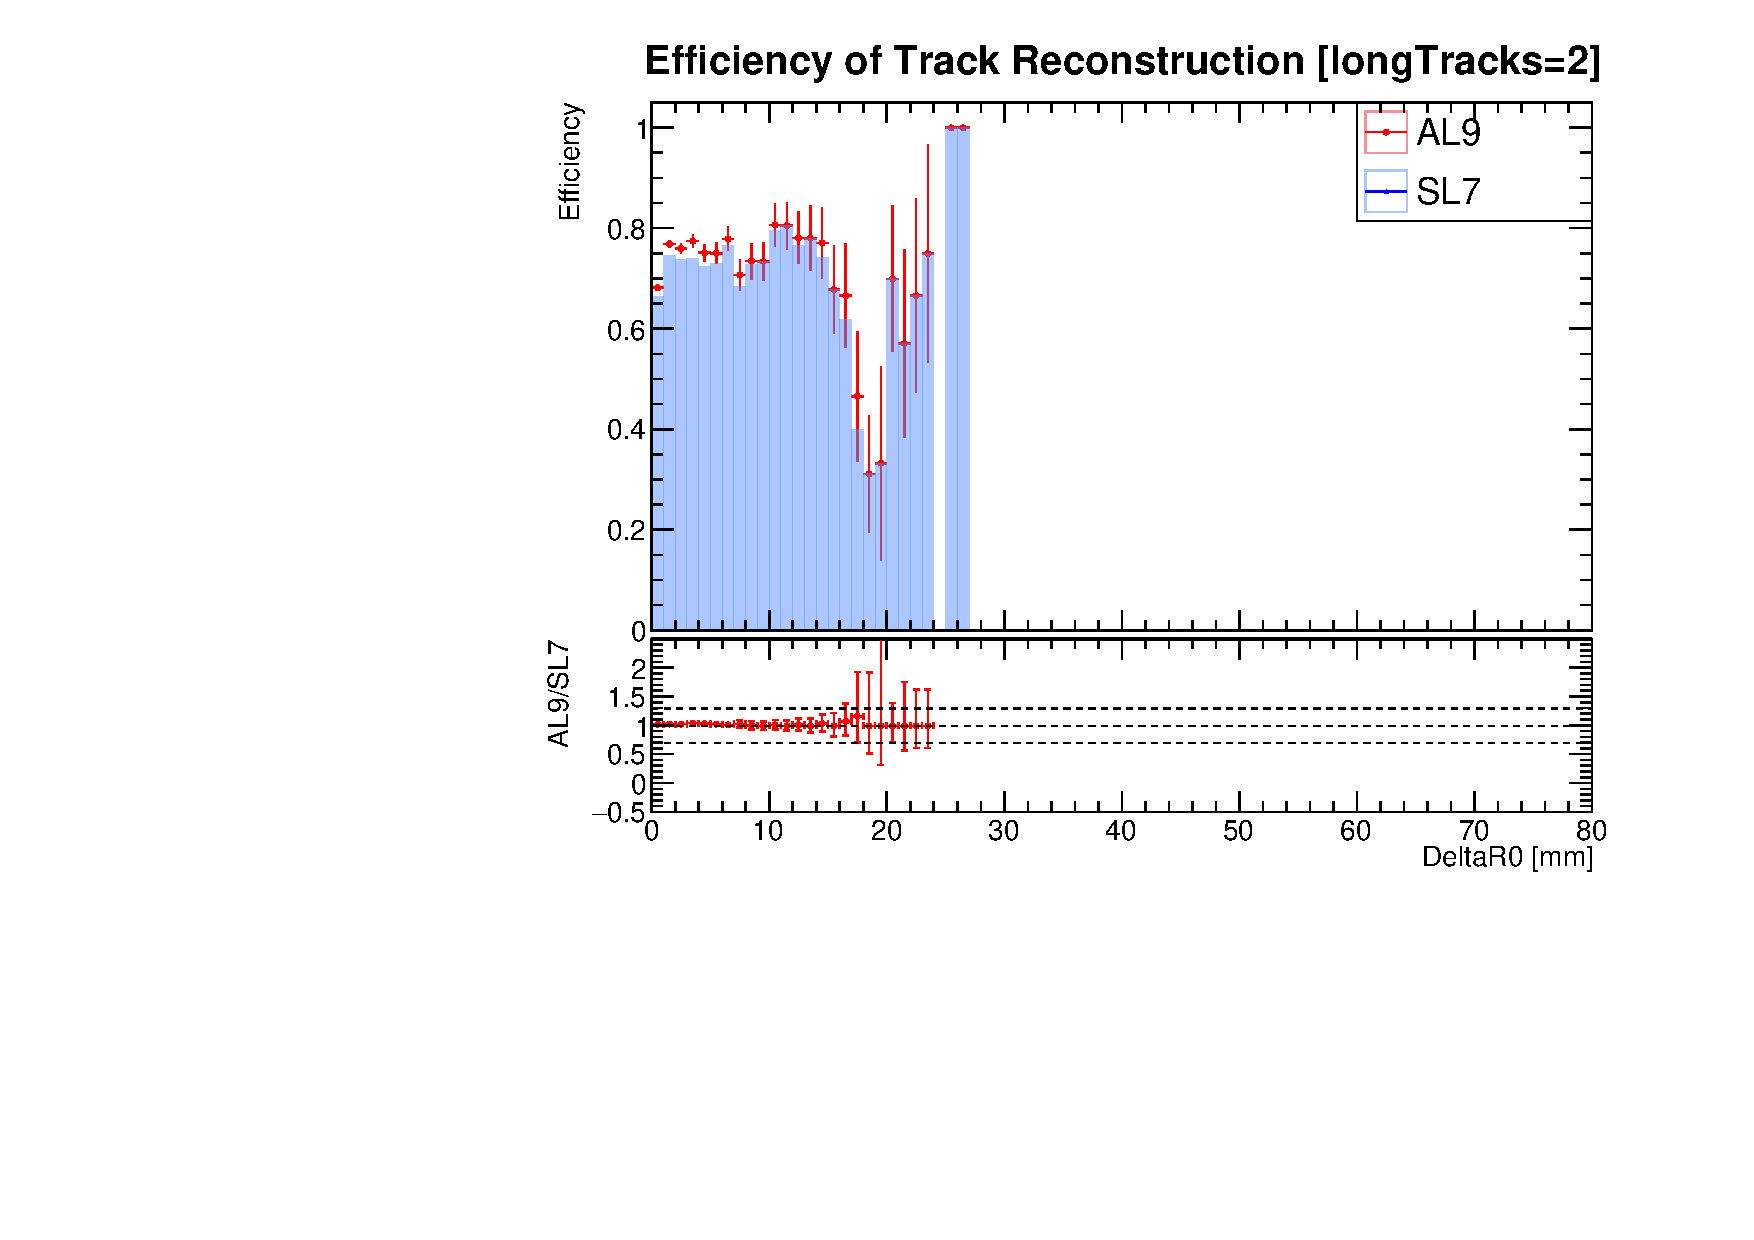
\includegraphics[width=\linewidth]{./output/Effi_eq2_DeltaR0.pdf}
    \end{figure}
\end{frame}
\begin{frame}{2 Track Efficiency as a function of DeltaX0 [SKIP]}
    \begin{figure}
        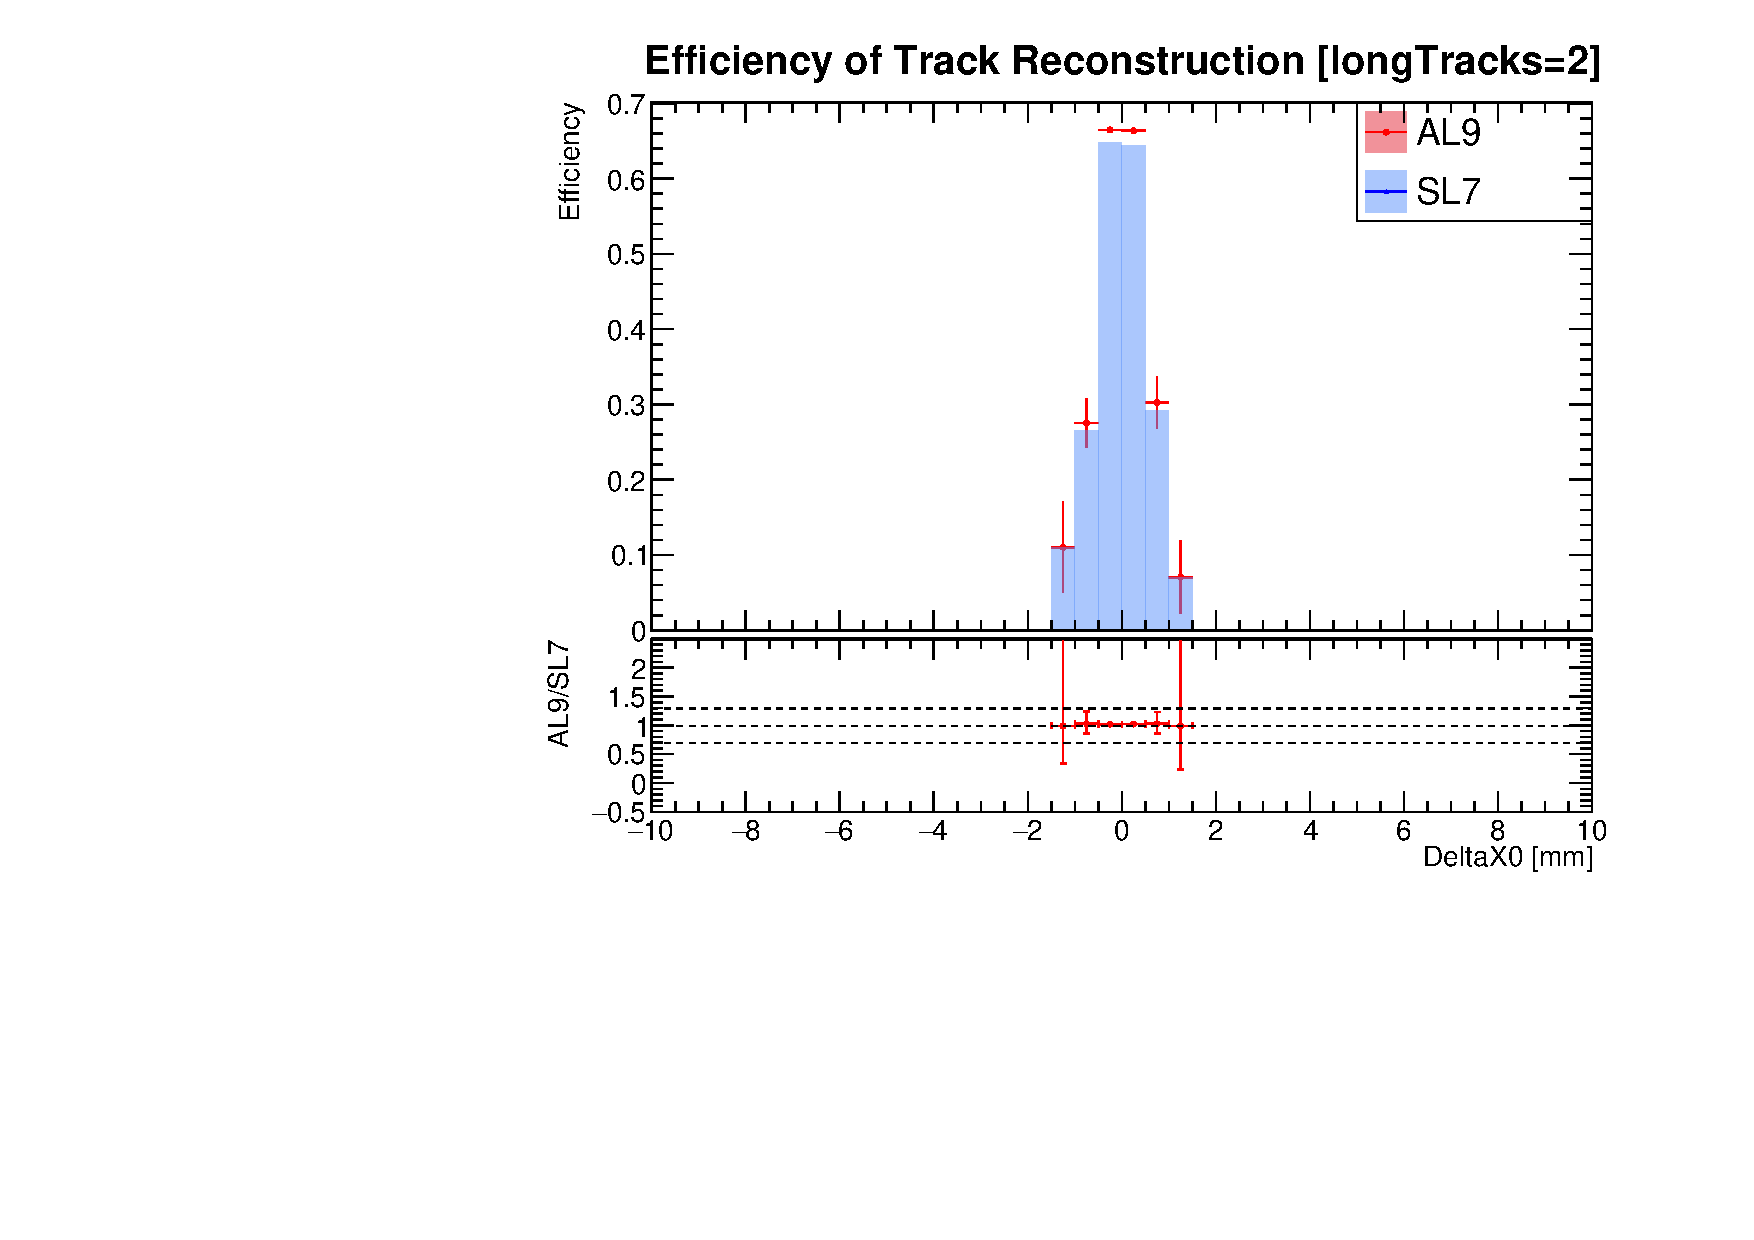
\includegraphics[width=\linewidth]{./output/Effi_eq2_DeltaX0.pdf}

    \end{figure}
\end{frame}
\begin{frame}{2 Track Efficiency as a function of DeltaY0 [SKIP]}
    \begin{figure}
        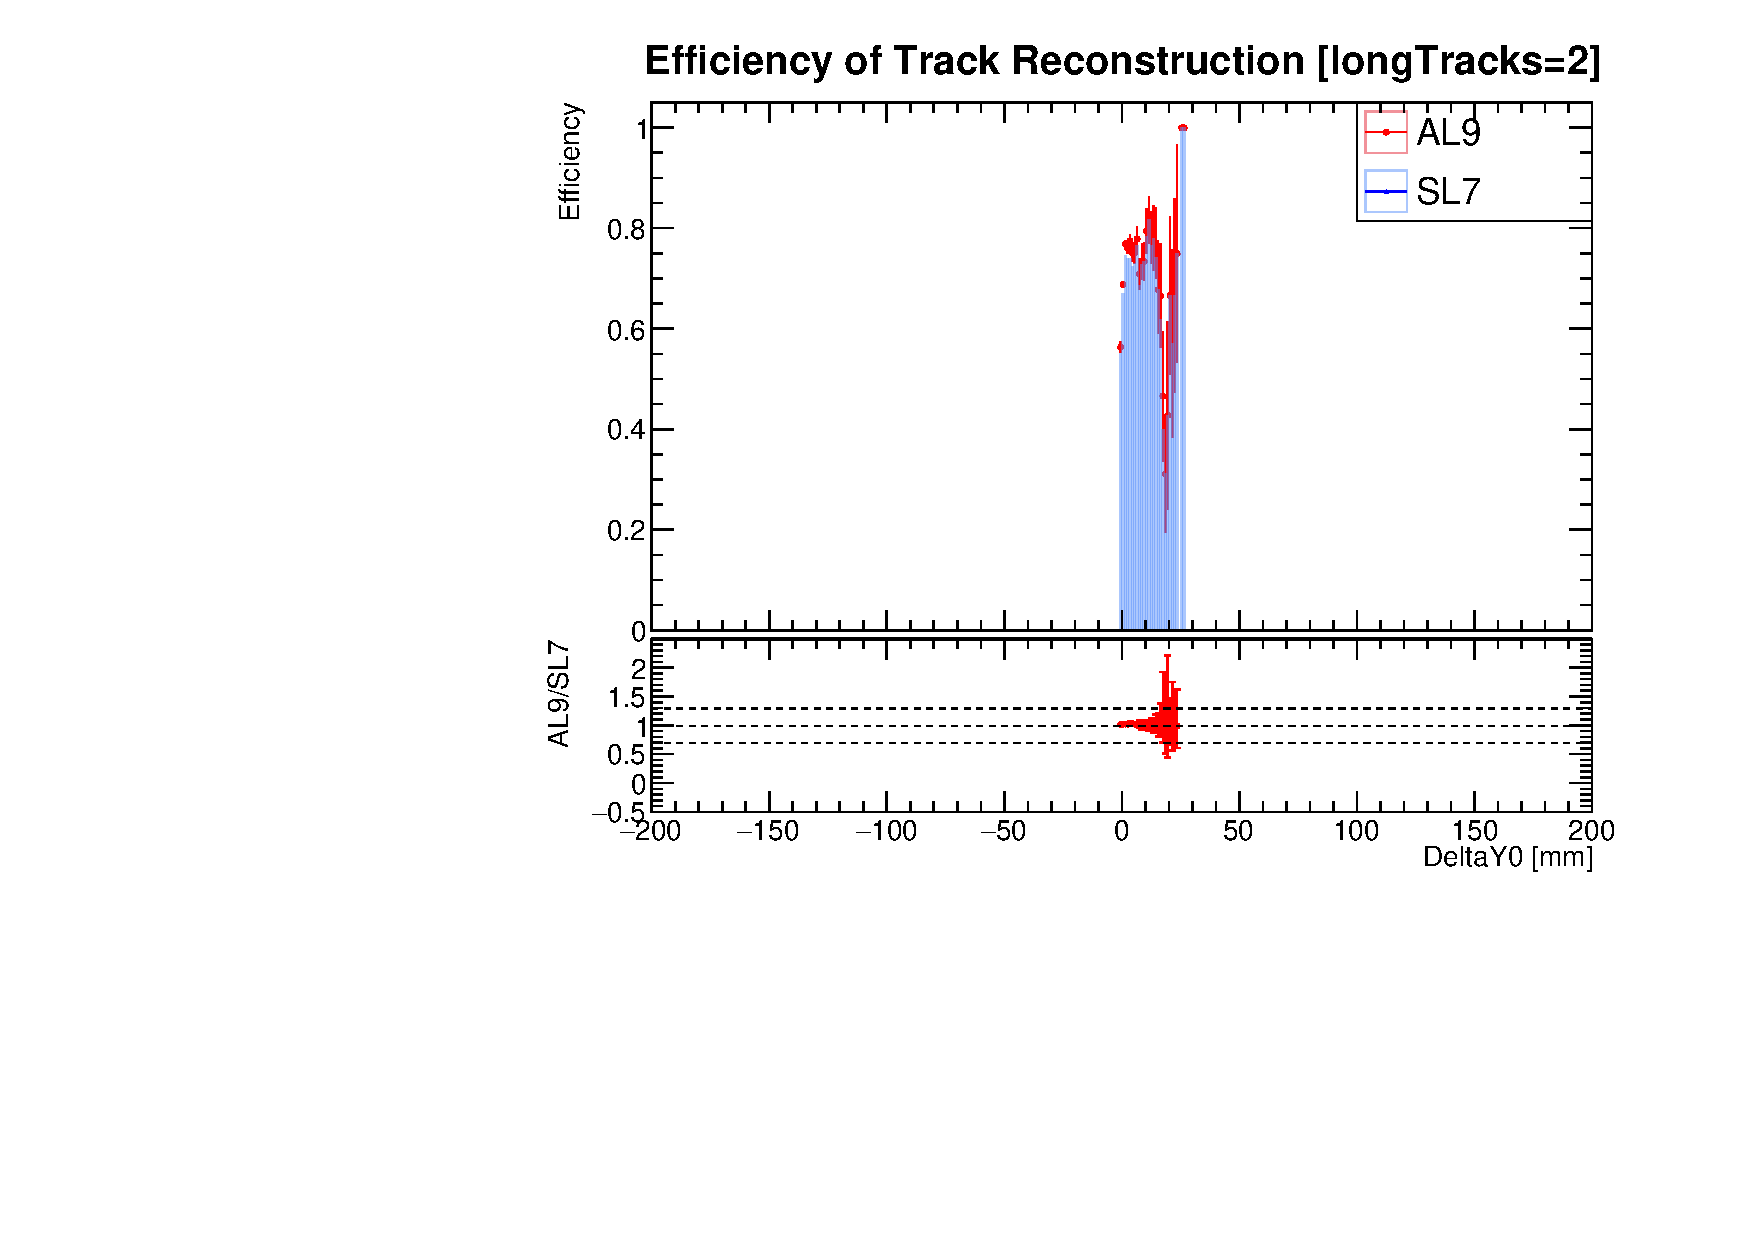
\includegraphics[width=\linewidth]{./output/Effi_eq2_DeltaY0.pdf}
    \end{figure}
\end{frame}
\begin{frame}{2 Track Efficiency as a function of Theta0}
    \begin{figure}
        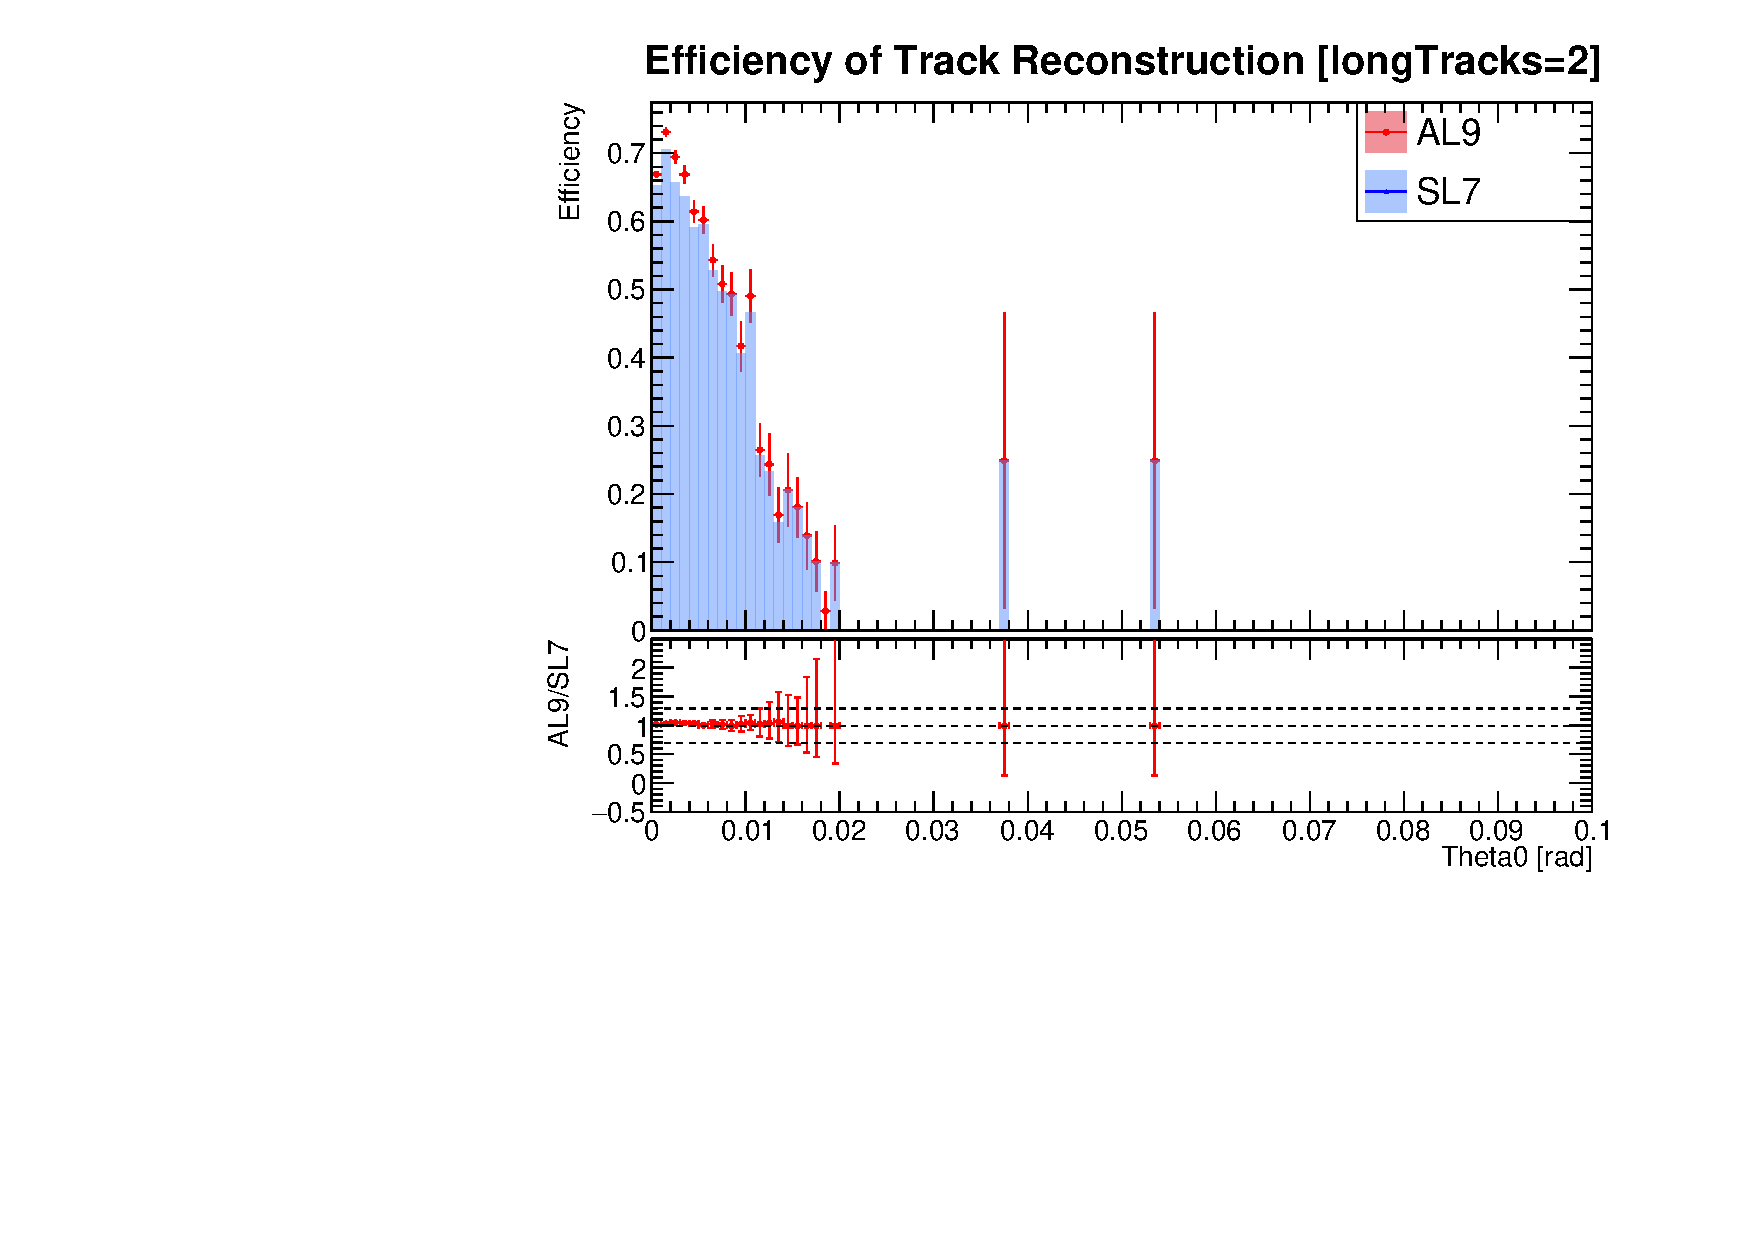
\includegraphics[width=\linewidth]{./output/Effi_eq2_Theta0.pdf}
    \end{figure}
\end{frame}
\begin{frame}{2 Track Efficiency as a function of DeltaRP}
    \begin{figure}
        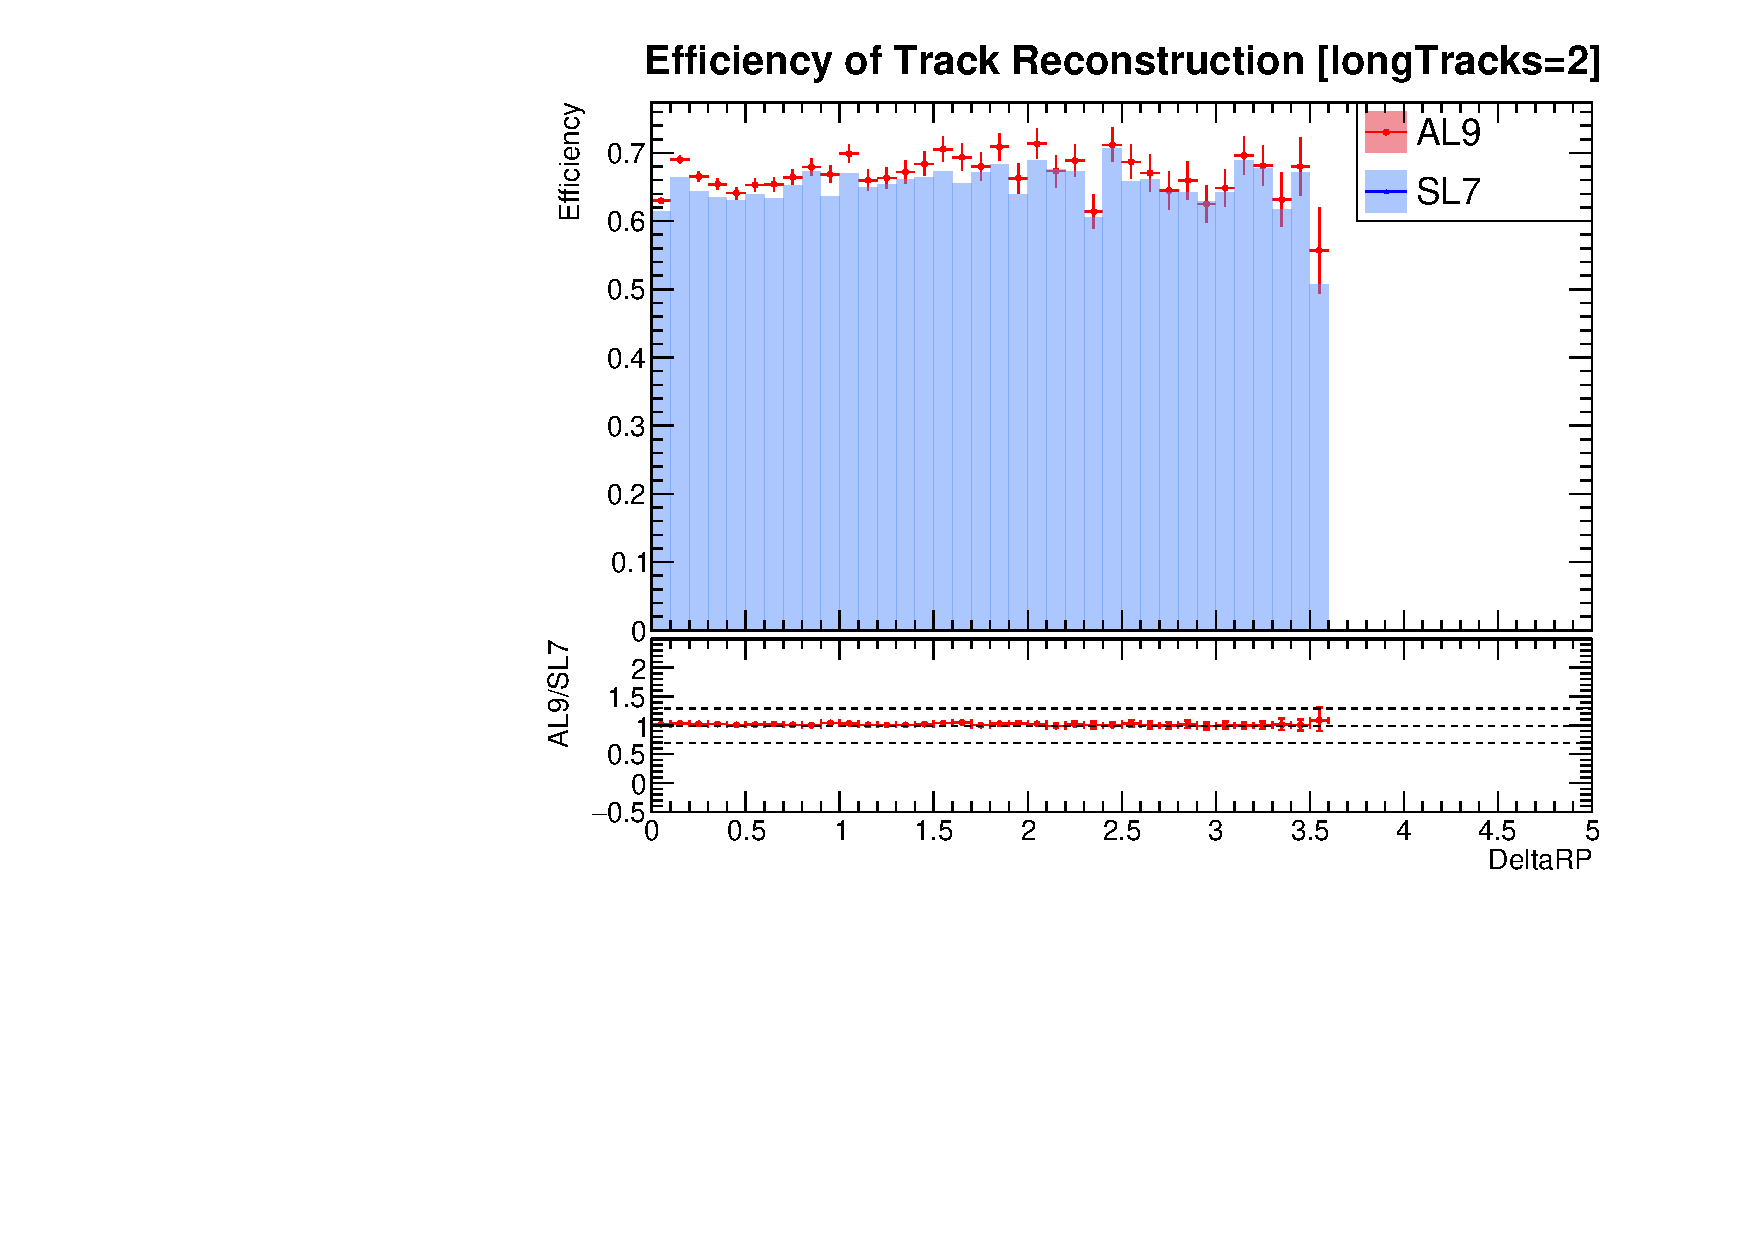
\includegraphics[width=\linewidth]{./output/Effi_eq2_DeltaRP.pdf}
    \end{figure}
\end{frame}

\begin{frame}{A More Robust Efficiency Metric [MC Based]}
    \begin{itemize}
        \item Our interest is only in the primary two tracks from $e^+e^-$
        \item For acceptance: Truth Position of $e^+e^-$ $<$ 100
        \item \text{\color{red}{\textbf{Identify the two primary tracks}} }
        \begin{itemize}
            \item Wanted to use t\_pdg\_parent \ldots
            \item Find closest to truth (by position and momenta)\dots 
            \item not trivial what is the margin of allowed error?
            \item Highest momenta tracks?
            \item Best approach is to use t\_truthHitRatio + PID
        \end{itemize}
        \item Can further quantify the ``goodness'' of the reconstructed primary tracks
    \end{itemize}
\end{frame}

\begin{frame}{Distribution of t\_pdg\_parent}
    \begin{table}[h!]
        \centering
        \small
        \begin{tabular}{|c|c|c|}
        \hline
        t\_pdg\_parent  & AL9       & SL7       \\ \hline
        -11             & 2         & 0         \\
        0               & 2         & 0         \\
        22              & 2610      & 2397      \\
        32              & 115877    & 112809    \\ \hline
        \end{tabular}
        \caption{Count of t\_pdg\_parent}
        \label{table:truth_efficiency}
        All particles are daughters of the Dark Photon? 
    \end{table}
    
\end{frame}

\section{Dark Photon CutFlow from Ansh's Study [SKIP]}
% \begin{frame}
    \includepdf[pages={3-5}]{assets/Alma9vsCentos7Efficiencies.pdf}
% \end{frame}

\begin{frame}{Comments on Data in NTuples [SKIP]}
    \begin{itemize}
        \item Need to add newly introducted variables to twiki.
        \item t\_st0\_x, y, z are filled with NaNs, We donot use/store station0 vals?
        \item t\_pdg\_parent ???
        \item truthParticleMatchedTracks - What exactly is this column.?
    \end{itemize}
    
\end{frame}

\section{Backup}
\appendix
\appendsubframes

\end{document}